\documentclass[twoside]{book}

% Packages required by doxygen
\usepackage{fixltx2e}
\usepackage{calc}
\usepackage{doxygen}
\usepackage[export]{adjustbox} % also loads graphicx
\usepackage{graphicx}
\usepackage[utf8]{inputenc}
\usepackage{makeidx}
\usepackage{multicol}
\usepackage{multirow}
\PassOptionsToPackage{warn}{textcomp}
\usepackage{textcomp}
\usepackage[nointegrals]{wasysym}
\usepackage[table]{xcolor}

% NLS support packages
\usepackage[french]{babel}

% Font selection
\usepackage[T1]{fontenc}
\usepackage[scaled=.90]{helvet}
\usepackage{courier}
\usepackage{amssymb}
\usepackage{sectsty}
\renewcommand{\familydefault}{\sfdefault}
\allsectionsfont{%
  \fontseries{bc}\selectfont%
  \color{darkgray}%
}
\renewcommand{\DoxyLabelFont}{%
  \fontseries{bc}\selectfont%
  \color{darkgray}%
}
\newcommand{\+}{\discretionary{\mbox{\scriptsize$\hookleftarrow$}}{}{}}

% Page & text layout
\usepackage{geometry}
\geometry{%
  a4paper,%
  top=2.5cm,%
  bottom=2.5cm,%
  left=2.5cm,%
  right=2.5cm%
}
\tolerance=750
\hfuzz=15pt
\hbadness=750
\setlength{\emergencystretch}{15pt}
\setlength{\parindent}{0cm}
\setlength{\parskip}{3ex plus 2ex minus 2ex}
\makeatletter
\renewcommand{\paragraph}{%
  \@startsection{paragraph}{4}{0ex}{-1.0ex}{1.0ex}{%
    \normalfont\normalsize\bfseries\SS@parafont%
  }%
}
\renewcommand{\subparagraph}{%
  \@startsection{subparagraph}{5}{0ex}{-1.0ex}{1.0ex}{%
    \normalfont\normalsize\bfseries\SS@subparafont%
  }%
}
\makeatother

% Headers & footers
\usepackage{fancyhdr}
\pagestyle{fancyplain}
\fancyhead[LE]{\fancyplain{}{\bfseries\thepage}}
\fancyhead[CE]{\fancyplain{}{}}
\fancyhead[RE]{\fancyplain{}{\bfseries\leftmark}}
\fancyhead[LO]{\fancyplain{}{\bfseries\rightmark}}
\fancyhead[CO]{\fancyplain{}{}}
\fancyhead[RO]{\fancyplain{}{\bfseries\thepage}}
\fancyfoot[LE]{\fancyplain{}{}}
\fancyfoot[CE]{\fancyplain{}{}}
\fancyfoot[RE]{\fancyplain{}{\bfseries\scriptsize Généré par Doxygen }}
\fancyfoot[LO]{\fancyplain{}{\bfseries\scriptsize Généré par Doxygen }}
\fancyfoot[CO]{\fancyplain{}{}}
\fancyfoot[RO]{\fancyplain{}{}}
\renewcommand{\footrulewidth}{0.4pt}
\renewcommand{\chaptermark}[1]{%
  \markboth{#1}{}%
}
\renewcommand{\sectionmark}[1]{%
  \markright{\thesection\ #1}%
}

% Indices & bibliography
\usepackage{natbib}
\usepackage[titles]{tocloft}
\setcounter{tocdepth}{3}
\setcounter{secnumdepth}{5}
\makeindex

% Hyperlinks (required, but should be loaded last)
\usepackage{ifpdf}
\ifpdf
  \usepackage[pdftex,pagebackref=true]{hyperref}
\else
  \usepackage[ps2pdf,pagebackref=true]{hyperref}
\fi
\hypersetup{%
  colorlinks=true,%
  linkcolor=blue,%
  citecolor=blue,%
  unicode%
}

% Custom commands
\newcommand{\clearemptydoublepage}{%
  \newpage{\pagestyle{empty}\cleardoublepage}%
}

\usepackage{caption}
\captionsetup{labelsep=space,justification=centering,font={bf},singlelinecheck=off,skip=4pt,position=top}

%===== C O N T E N T S =====

\begin{document}

% Titlepage & ToC
\hypersetup{pageanchor=false,
             bookmarksnumbered=true,
             pdfencoding=unicode
            }
\pagenumbering{alph}
\begin{titlepage}
\vspace*{7cm}
\begin{center}%
{\Large Schmou\textquotesingle{}T\+SE }\\
\vspace*{1cm}
{\large Généré par Doxygen 1.8.13}\\
\end{center}
\end{titlepage}
\clearemptydoublepage
\pagenumbering{roman}
\tableofcontents
\clearemptydoublepage
\pagenumbering{arabic}
\hypersetup{pageanchor=true}

%--- Begin generated contents ---
\chapter{Index hiérarchique}
\section{Class Hierarchy}
This inheritance list is sorted roughly, but not completely, alphabetically\+:\begin{DoxyCompactList}
\item \contentsline{section}{Bouton\+Capacite}{\pageref{class_bouton_capacite}}{}
\item \contentsline{section}{Capacite}{\pageref{class_capacite}}{}
\begin{DoxyCompactList}
\item \contentsline{section}{Cap\+Aim\+Bot}{\pageref{class_cap_aim_bot}}{}
\item \contentsline{section}{Cap\+Bismillah}{\pageref{class_cap_bismillah}}{}
\item \contentsline{section}{Cap\+Boing}{\pageref{class_cap_boing}}{}
\item \contentsline{section}{Cap\+Bouclier\+Rond}{\pageref{class_cap_bouclier_rond}}{}
\item \contentsline{section}{Cap\+Dash}{\pageref{class_cap_dash}}{}
\item \contentsline{section}{Cap\+Missile}{\pageref{class_cap_missile}}{}
\item \contentsline{section}{Cap\+Piou}{\pageref{class_cap_piou}}{}
\end{DoxyCompactList}
\item \contentsline{section}{case\+Insensitive\+Compare}{\pageref{structcase_insensitive_compare}}{}
\item \contentsline{section}{Chargeur}{\pageref{class_chargeur}}{}
\item \contentsline{section}{std\+:\+:experimental\+:\+:constexpr\+\_\+optional\+\_\+base$<$ T $>$}{\pageref{structstd_1_1experimental_1_1constexpr__optional__base}}{}
\item \contentsline{section}{std\+:\+:experimental\+:\+:constexpr\+\_\+storage\+\_\+t$<$ T $>$}{\pageref{unionstd_1_1experimental_1_1constexpr__storage__t}}{}
\item \contentsline{section}{Ecran}{\pageref{class_ecran}}{}
\begin{DoxyCompactList}
\item \contentsline{section}{Accueil}{\pageref{class_accueil}}{}
\item \contentsline{section}{Menu\+Principal}{\pageref{class_menu_principal}}{}
\item \contentsline{section}{Partie}{\pageref{class_partie}}{}
\begin{DoxyCompactList}
\item \contentsline{section}{Pattern}{\pageref{class_pattern}}{}
\end{DoxyCompactList}
\end{DoxyCompactList}
\item \contentsline{section}{Element\+Vague}{\pageref{struct_element_vague}}{}
\item \contentsline{section}{Entite}{\pageref{class_entite}}{}
\begin{DoxyCompactList}
\item \contentsline{section}{Projectile}{\pageref{class_projectile}}{}
\begin{DoxyCompactList}
\item \contentsline{section}{Proj\+Bismillah}{\pageref{class_proj_bismillah}}{}
\item \contentsline{section}{Proj\+Boing}{\pageref{class_proj_boing}}{}
\item \contentsline{section}{Proj\+Bouclier\+Rond}{\pageref{class_proj_bouclier_rond}}{}
\item \contentsline{section}{Proj\+Missile}{\pageref{class_proj_missile}}{}
\item \contentsline{section}{Proj\+Piou}{\pageref{class_proj_piou}}{}
\end{DoxyCompactList}
\item \contentsline{section}{Vaisseau}{\pageref{class_vaisseau}}{}
\begin{DoxyCompactList}
\item \contentsline{section}{Vaiss\+Bouclier}{\pageref{class_vaiss_bouclier}}{}
\item \contentsline{section}{Vaisseau\+Attaquant}{\pageref{class_vaisseau_attaquant}}{}
\item \contentsline{section}{Vaisseau\+Defenseur}{\pageref{class_vaisseau_defenseur}}{}
\item \contentsline{section}{Vaisseau\+Eclaireur}{\pageref{class_vaisseau_eclaireur}}{}
\item \contentsline{section}{Vaisseau\+Test}{\pageref{class_vaisseau_test}}{}
\end{DoxyCompactList}
\end{DoxyCompactList}
\item \contentsline{section}{std\+:\+:experimental\+:\+:is\+\_\+nothrow\+\_\+move\+\_\+assignable$<$ T $>$\+:\+:has\+\_\+nothrow\+\_\+move\+\_\+assign$<$ X, has\+\_\+any\+\_\+move\+\_\+assign $>$}{\pageref{structstd_1_1experimental_1_1is__nothrow__move__assignable_1_1has__nothrow__move__assign}}{}
\item \contentsline{section}{std\+:\+:experimental\+:\+:is\+\_\+nothrow\+\_\+move\+\_\+assignable$<$ T $>$\+:\+:has\+\_\+nothrow\+\_\+move\+\_\+assign$<$ X, true $>$}{\pageref{structstd_1_1experimental_1_1is__nothrow__move__assignable_1_1has__nothrow__move__assign_3_01_x_00_01true_01_4}}{}
\item \contentsline{section}{std\+:\+:experimental\+:\+:detail\+\_\+\+:\+:has\+\_\+overloaded\+\_\+addressof$<$ T $>$}{\pageref{structstd_1_1experimental_1_1detail___1_1has__overloaded__addressof}}{}
\item \contentsline{section}{std\+:\+:hash$<$ std\+:\+:experimental\+:\+:optional$<$ T \& $>$ $>$}{\pageref{structstd_1_1hash_3_01std_1_1experimental_1_1optional_3_01_t_01_6_01_4_01_4}}{}
\item \contentsline{section}{std\+:\+:hash$<$ std\+:\+:experimental\+:\+:optional$<$ T $>$ $>$}{\pageref{structstd_1_1hash_3_01std_1_1experimental_1_1optional_3_01_t_01_4_01_4}}{}
\item \contentsline{section}{std\+:\+:experimental\+:\+:in\+\_\+place\+\_\+t}{\pageref{structstd_1_1experimental_1_1in__place__t}}{}
\item \contentsline{section}{std\+:\+:experimental\+:\+:nullopt\+\_\+t\+:\+:init}{\pageref{structstd_1_1experimental_1_1nullopt__t_1_1init}}{}
\item \contentsline{section}{Input\+\_\+base$<$ N $>$}{\pageref{class_input__base}}{}
\item \contentsline{section}{Input\+\_\+base$<$ N\+B\+\_\+\+A\+C\+T\+I\+ON $>$}{\pageref{class_input__base}}{}
\item \contentsline{section}{std\+:\+:experimental\+:\+:is\+\_\+assignable$<$ T, U $>$}{\pageref{structstd_1_1experimental_1_1is__assignable}}{}
\item \contentsline{section}{std\+:\+:experimental\+:\+:is\+\_\+nothrow\+\_\+move\+\_\+assignable$<$ T $>$}{\pageref{structstd_1_1experimental_1_1is__nothrow__move__assignable}}{}
\item \contentsline{section}{std\+:\+:experimental\+:\+:is\+\_\+nothrow\+\_\+move\+\_\+constructible$<$ T $>$}{\pageref{structstd_1_1experimental_1_1is__nothrow__move__constructible}}{}
\item logic\+\_\+error\begin{DoxyCompactList}
\item \contentsline{section}{std\+:\+:experimental\+:\+:bad\+\_\+optional\+\_\+access}{\pageref{classstd_1_1experimental_1_1bad__optional__access}}{}
\end{DoxyCompactList}
\item \contentsline{section}{std\+:\+:experimental\+:\+:nullopt\+\_\+t}{\pageref{structstd_1_1experimental_1_1nullopt__t}}{}
\item \contentsline{section}{std\+:\+:experimental\+:\+:optional$<$ T \& $>$}{\pageref{classstd_1_1experimental_1_1optional_3_01_t_01_6_01_4}}{}
\item \contentsline{section}{std\+:\+:experimental\+:\+:optional$<$ T \&\& $>$}{\pageref{classstd_1_1experimental_1_1optional_3_01_t_01_6_6_01_4}}{}
\item \contentsline{section}{std\+:\+:experimental\+:\+:optional\+\_\+base$<$ T $>$}{\pageref{structstd_1_1experimental_1_1optional__base}}{}
\item Optional\+Base\begin{DoxyCompactList}
\item \contentsline{section}{std\+:\+:experimental\+:\+:optional$<$ unsigned int $>$}{\pageref{classstd_1_1experimental_1_1optional}}{}
\item \contentsline{section}{std\+:\+:experimental\+:\+:optional$<$ T $>$}{\pageref{classstd_1_1experimental_1_1optional}}{}
\end{DoxyCompactList}
\item \contentsline{section}{Overlay}{\pageref{class_overlay}}{}
\item \contentsline{section}{Stats}{\pageref{struct_stats}}{}
\item \contentsline{section}{std\+:\+:experimental\+:\+:storage\+\_\+t$<$ T $>$}{\pageref{unionstd_1_1experimental_1_1storage__t}}{}
\item \contentsline{section}{std\+:\+:experimental\+:\+:trivial\+\_\+init\+\_\+t}{\pageref{structstd_1_1experimental_1_1trivial__init__t}}{}
\item \contentsline{section}{Vague}{\pageref{class_vague}}{}
\item \contentsline{section}{Vaisseau\+Bouclier}{\pageref{class_vaisseau_bouclier}}{}
\end{DoxyCompactList}

\chapter{Index des classes}
\section{Liste des classes}
Liste des classes, structures, unions et interfaces avec une brève description \+:\begin{DoxyCompactList}
\item\contentsline{section}{\hyperlink{class_capacite}{Capacite} \\*Classe abstraite qui définit la structure générale d\textquotesingle{}une capacité, à faire hériter de chaque capacité }{\pageref{class_capacite}}{}
\item\contentsline{section}{\hyperlink{class_cap_dash}{Cap\+Dash} \\*Classe Capacité permettant de dash }{\pageref{class_cap_dash}}{}
\item\contentsline{section}{\hyperlink{class_cap_piou}{Cap\+Piou} \\*Classe Capacité de base }{\pageref{class_cap_piou}}{}
\item\contentsline{section}{\hyperlink{class_cap_test}{Cap\+Test} \\*Classe Capacité de test }{\pageref{class_cap_test}}{}
\item\contentsline{section}{\hyperlink{class_entite}{Entite} \\*Classe virtuelle qui définit une entité }{\pageref{class_entite}}{}
\item\contentsline{section}{\hyperlink{class_input__base}{Input\+\_\+base$<$ N $>$} }{\pageref{class_input__base}}{}
\item\contentsline{section}{\hyperlink{class_partie}{Partie} \\*Description brève }{\pageref{class_partie}}{}
\item\contentsline{section}{\hyperlink{class_projectile}{Projectile} \\*Classe abstraite qui définit la structure générale d\textquotesingle{}un projectile, à faire hériter pour chaque projectile }{\pageref{class_projectile}}{}
\item\contentsline{section}{\hyperlink{class_proj_piou}{Proj\+Piou} \\*\hyperlink{class_projectile}{Projectile} de test }{\pageref{class_proj_piou}}{}
\item\contentsline{section}{\hyperlink{class_proj_test}{Proj\+Test} \\*\hyperlink{class_projectile}{Projectile} de test }{\pageref{class_proj_test}}{}
\item\contentsline{section}{\hyperlink{class_vaisseau}{Vaisseau} \\*Classe du vaisseau (véhicule) d\textquotesingle{}un joueur ou d\textquotesingle{}un ennemi }{\pageref{class_vaisseau}}{}
\item\contentsline{section}{\hyperlink{class_vaisseau_eclaireur}{Vaisseau\+Eclaireur} \\*Classe d\textquotesingle{}un ennemi de base \+: l\textquotesingle{}�claireur }{\pageref{class_vaisseau_eclaireur}}{}
\item\contentsline{section}{\hyperlink{class_vaisseau_test}{Vaisseau\+Test} }{\pageref{class_vaisseau_test}}{}
\end{DoxyCompactList}

\chapter{Index des fichiers}
\section{Liste des fichiers}
Liste de tous les fichiers avec une brève description \+:\begin{DoxyCompactList}
\item\contentsline{section}{src/\hyperlink{___capacites_8h}{\+\_\+\+Capacites.\+h} }{\pageref{___capacites_8h}}{}
\item\contentsline{section}{src/\hyperlink{__projectiles_8h}{\+\_\+projectiles.\+h} }{\pageref{__projectiles_8h}}{}
\item\contentsline{section}{src/\hyperlink{_attaque_8h}{Attaque.\+h} }{\pageref{_attaque_8h}}{}
\item\contentsline{section}{src/\hyperlink{_capacite_8cpp}{Capacite.\+cpp} }{\pageref{_capacite_8cpp}}{}
\item\contentsline{section}{src/\hyperlink{_capacite_8h}{Capacite.\+h} }{\pageref{_capacite_8h}}{}
\item\contentsline{section}{src/\hyperlink{_capacite_piou_piou_8cpp}{Capacite\+Piou\+Piou.\+cpp} }{\pageref{_capacite_piou_piou_8cpp}}{}
\item\contentsline{section}{src/\hyperlink{_capacite_piou_piou_8h}{Capacite\+Piou\+Piou.\+h} }{\pageref{_capacite_piou_piou_8h}}{}
\item\contentsline{section}{src/\hyperlink{_cap_dash_8cpp}{Cap\+Dash.\+cpp} }{\pageref{_cap_dash_8cpp}}{}
\item\contentsline{section}{src/\hyperlink{_cap_dash_8h}{Cap\+Dash.\+h} }{\pageref{_cap_dash_8h}}{}
\item\contentsline{section}{src/\hyperlink{_cap_piou_8cpp}{Cap\+Piou.\+cpp} }{\pageref{_cap_piou_8cpp}}{}
\item\contentsline{section}{src/\hyperlink{_cap_piou_8h}{Cap\+Piou.\+h} }{\pageref{_cap_piou_8h}}{}
\item\contentsline{section}{src/\hyperlink{_cap_test_8cpp}{Cap\+Test.\+cpp} }{\pageref{_cap_test_8cpp}}{}
\item\contentsline{section}{src/\hyperlink{_cap_test_8h}{Cap\+Test.\+h} }{\pageref{_cap_test_8h}}{}
\item\contentsline{section}{src/\hyperlink{_collision_8cpp}{Collision.\+cpp} }{\pageref{_collision_8cpp}}{}
\item\contentsline{section}{src/\hyperlink{_collision_8h}{Collision.\+h} }{\pageref{_collision_8h}}{}
\item\contentsline{section}{src/\hyperlink{constantes_8h}{constantes.\+h} }{\pageref{constantes_8h}}{}
\item\contentsline{section}{src/\hyperlink{_entite_8cpp}{Entite.\+cpp} }{\pageref{_entite_8cpp}}{}
\item\contentsline{section}{src/\hyperlink{_entite_8h}{Entite.\+h} }{\pageref{_entite_8h}}{}
\item\contentsline{section}{src/\hyperlink{_input_8cpp}{Input.\+cpp} }{\pageref{_input_8cpp}}{}
\item\contentsline{section}{src/\hyperlink{_input_8h}{Input.\+h} }{\pageref{_input_8h}}{}
\item\contentsline{section}{src/\hyperlink{main_8cpp}{main.\+cpp} }{\pageref{main_8cpp}}{}
\item\contentsline{section}{src/\hyperlink{_partie_8cpp}{Partie.\+cpp} }{\pageref{_partie_8cpp}}{}
\item\contentsline{section}{src/\hyperlink{_partie_8h}{Partie.\+h} }{\pageref{_partie_8h}}{}
\item\contentsline{section}{src/\hyperlink{_projectile_8cpp}{Projectile.\+cpp} }{\pageref{_projectile_8cpp}}{}
\item\contentsline{section}{src/\hyperlink{_projectile_8h}{Projectile.\+h} }{\pageref{_projectile_8h}}{}
\item\contentsline{section}{src/\hyperlink{_projectile_piou_piou_8cpp}{Projectile\+Piou\+Piou.\+cpp} }{\pageref{_projectile_piou_piou_8cpp}}{}
\item\contentsline{section}{src/\hyperlink{_projectile_piou_piou_8h}{Projectile\+Piou\+Piou.\+h} }{\pageref{_projectile_piou_piou_8h}}{}
\item\contentsline{section}{src/\hyperlink{_proj_piou_8cpp}{Proj\+Piou.\+cpp} }{\pageref{_proj_piou_8cpp}}{}
\item\contentsline{section}{src/\hyperlink{_proj_piou_8h}{Proj\+Piou.\+h} }{\pageref{_proj_piou_8h}}{}
\item\contentsline{section}{src/\hyperlink{_proj_test_8cpp}{Proj\+Test.\+cpp} }{\pageref{_proj_test_8cpp}}{}
\item\contentsline{section}{src/\hyperlink{_proj_test_8h}{Proj\+Test.\+h} }{\pageref{_proj_test_8h}}{}
\item\contentsline{section}{src/\hyperlink{_vaisseau_8cpp}{Vaisseau.\+cpp} }{\pageref{_vaisseau_8cpp}}{}
\item\contentsline{section}{src/\hyperlink{_vaisseau_8h}{Vaisseau.\+h} }{\pageref{_vaisseau_8h}}{}
\item\contentsline{section}{src/\hyperlink{_vaisseau_test_8cpp}{Vaisseau\+Test.\+cpp} }{\pageref{_vaisseau_test_8cpp}}{}
\item\contentsline{section}{src/\hyperlink{_vaisseau_test_8h}{Vaisseau\+Test.\+h} }{\pageref{_vaisseau_test_8h}}{}
\end{DoxyCompactList}

\chapter{Documentation des classes}
\hypertarget{struct_input__base_1_1movement__input__t_1_1joypad__t_1_1joypad__input__t_1_1buttons__t}{}\section{Référence de la structure Input\+\_\+base$<$ N $>$\+:\+:movement\+\_\+input\+\_\+t\+:\+:joypad\+\_\+t\+:\+:joypad\+\_\+input\+\_\+t\+:\+:buttons\+\_\+t}
\label{struct_input__base_1_1movement__input__t_1_1joypad__t_1_1joypad__input__t_1_1buttons__t}\index{Input\+\_\+base$<$ N $>$\+::movement\+\_\+input\+\_\+t\+::joypad\+\_\+t\+::joypad\+\_\+input\+\_\+t\+::buttons\+\_\+t@{Input\+\_\+base$<$ N $>$\+::movement\+\_\+input\+\_\+t\+::joypad\+\_\+t\+::joypad\+\_\+input\+\_\+t\+::buttons\+\_\+t}}


{\ttfamily \#include $<$Input.\+h$>$}

\subsection*{Attributs publics}
\begin{DoxyCompactItemize}
\item 
std\+::optional$<$ unsigned int $>$ \hyperlink{struct_input__base_1_1movement__input__t_1_1joypad__t_1_1joypad__input__t_1_1buttons__t_a239929c919634205fe86f61208515848}{up\+\_\+button\+\_\+}
\item 
std\+::optional$<$ unsigned int $>$ \hyperlink{struct_input__base_1_1movement__input__t_1_1joypad__t_1_1joypad__input__t_1_1buttons__t_a3c344e2a9fdce4a396d22af8a4be1df0}{down\+\_\+button\+\_\+}
\item 
std\+::optional$<$ unsigned int $>$ \hyperlink{struct_input__base_1_1movement__input__t_1_1joypad__t_1_1joypad__input__t_1_1buttons__t_a99d61f77f1486465196c4279d23f1bff}{left\+\_\+button\+\_\+}
\item 
std\+::optional$<$ unsigned int $>$ \hyperlink{struct_input__base_1_1movement__input__t_1_1joypad__t_1_1joypad__input__t_1_1buttons__t_a97e4219d56eb1f5fd903e391af1e65c8}{right\+\_\+button\+\_\+}
\end{DoxyCompactItemize}


\subsection{Documentation des données membres}
\mbox{\Hypertarget{struct_input__base_1_1movement__input__t_1_1joypad__t_1_1joypad__input__t_1_1buttons__t_a3c344e2a9fdce4a396d22af8a4be1df0}\label{struct_input__base_1_1movement__input__t_1_1joypad__t_1_1joypad__input__t_1_1buttons__t_a3c344e2a9fdce4a396d22af8a4be1df0}} 
\index{Input\+\_\+base\+::movement\+\_\+input\+\_\+t\+::joypad\+\_\+t\+::joypad\+\_\+input\+\_\+t\+::buttons\+\_\+t@{Input\+\_\+base\+::movement\+\_\+input\+\_\+t\+::joypad\+\_\+t\+::joypad\+\_\+input\+\_\+t\+::buttons\+\_\+t}!down\+\_\+button\+\_\+@{down\+\_\+button\+\_\+}}
\index{down\+\_\+button\+\_\+@{down\+\_\+button\+\_\+}!Input\+\_\+base\+::movement\+\_\+input\+\_\+t\+::joypad\+\_\+t\+::joypad\+\_\+input\+\_\+t\+::buttons\+\_\+t@{Input\+\_\+base\+::movement\+\_\+input\+\_\+t\+::joypad\+\_\+t\+::joypad\+\_\+input\+\_\+t\+::buttons\+\_\+t}}
\subsubsection{\texorpdfstring{down\+\_\+button\+\_\+}{down\_button\_}}
{\footnotesize\ttfamily template$<$size\+\_\+t N$>$ \\
std\+::optional$<$unsigned int$>$ \hyperlink{class_input__base}{Input\+\_\+base}$<$ N $>$\+::movement\+\_\+input\+\_\+t\+::joypad\+\_\+t\+::joypad\+\_\+input\+\_\+t\+::buttons\+\_\+t\+::down\+\_\+button\+\_\+}

\mbox{\Hypertarget{struct_input__base_1_1movement__input__t_1_1joypad__t_1_1joypad__input__t_1_1buttons__t_a99d61f77f1486465196c4279d23f1bff}\label{struct_input__base_1_1movement__input__t_1_1joypad__t_1_1joypad__input__t_1_1buttons__t_a99d61f77f1486465196c4279d23f1bff}} 
\index{Input\+\_\+base\+::movement\+\_\+input\+\_\+t\+::joypad\+\_\+t\+::joypad\+\_\+input\+\_\+t\+::buttons\+\_\+t@{Input\+\_\+base\+::movement\+\_\+input\+\_\+t\+::joypad\+\_\+t\+::joypad\+\_\+input\+\_\+t\+::buttons\+\_\+t}!left\+\_\+button\+\_\+@{left\+\_\+button\+\_\+}}
\index{left\+\_\+button\+\_\+@{left\+\_\+button\+\_\+}!Input\+\_\+base\+::movement\+\_\+input\+\_\+t\+::joypad\+\_\+t\+::joypad\+\_\+input\+\_\+t\+::buttons\+\_\+t@{Input\+\_\+base\+::movement\+\_\+input\+\_\+t\+::joypad\+\_\+t\+::joypad\+\_\+input\+\_\+t\+::buttons\+\_\+t}}
\subsubsection{\texorpdfstring{left\+\_\+button\+\_\+}{left\_button\_}}
{\footnotesize\ttfamily template$<$size\+\_\+t N$>$ \\
std\+::optional$<$unsigned int$>$ \hyperlink{class_input__base}{Input\+\_\+base}$<$ N $>$\+::movement\+\_\+input\+\_\+t\+::joypad\+\_\+t\+::joypad\+\_\+input\+\_\+t\+::buttons\+\_\+t\+::left\+\_\+button\+\_\+}

\mbox{\Hypertarget{struct_input__base_1_1movement__input__t_1_1joypad__t_1_1joypad__input__t_1_1buttons__t_a97e4219d56eb1f5fd903e391af1e65c8}\label{struct_input__base_1_1movement__input__t_1_1joypad__t_1_1joypad__input__t_1_1buttons__t_a97e4219d56eb1f5fd903e391af1e65c8}} 
\index{Input\+\_\+base\+::movement\+\_\+input\+\_\+t\+::joypad\+\_\+t\+::joypad\+\_\+input\+\_\+t\+::buttons\+\_\+t@{Input\+\_\+base\+::movement\+\_\+input\+\_\+t\+::joypad\+\_\+t\+::joypad\+\_\+input\+\_\+t\+::buttons\+\_\+t}!right\+\_\+button\+\_\+@{right\+\_\+button\+\_\+}}
\index{right\+\_\+button\+\_\+@{right\+\_\+button\+\_\+}!Input\+\_\+base\+::movement\+\_\+input\+\_\+t\+::joypad\+\_\+t\+::joypad\+\_\+input\+\_\+t\+::buttons\+\_\+t@{Input\+\_\+base\+::movement\+\_\+input\+\_\+t\+::joypad\+\_\+t\+::joypad\+\_\+input\+\_\+t\+::buttons\+\_\+t}}
\subsubsection{\texorpdfstring{right\+\_\+button\+\_\+}{right\_button\_}}
{\footnotesize\ttfamily template$<$size\+\_\+t N$>$ \\
std\+::optional$<$unsigned int$>$ \hyperlink{class_input__base}{Input\+\_\+base}$<$ N $>$\+::movement\+\_\+input\+\_\+t\+::joypad\+\_\+t\+::joypad\+\_\+input\+\_\+t\+::buttons\+\_\+t\+::right\+\_\+button\+\_\+}

\mbox{\Hypertarget{struct_input__base_1_1movement__input__t_1_1joypad__t_1_1joypad__input__t_1_1buttons__t_a239929c919634205fe86f61208515848}\label{struct_input__base_1_1movement__input__t_1_1joypad__t_1_1joypad__input__t_1_1buttons__t_a239929c919634205fe86f61208515848}} 
\index{Input\+\_\+base\+::movement\+\_\+input\+\_\+t\+::joypad\+\_\+t\+::joypad\+\_\+input\+\_\+t\+::buttons\+\_\+t@{Input\+\_\+base\+::movement\+\_\+input\+\_\+t\+::joypad\+\_\+t\+::joypad\+\_\+input\+\_\+t\+::buttons\+\_\+t}!up\+\_\+button\+\_\+@{up\+\_\+button\+\_\+}}
\index{up\+\_\+button\+\_\+@{up\+\_\+button\+\_\+}!Input\+\_\+base\+::movement\+\_\+input\+\_\+t\+::joypad\+\_\+t\+::joypad\+\_\+input\+\_\+t\+::buttons\+\_\+t@{Input\+\_\+base\+::movement\+\_\+input\+\_\+t\+::joypad\+\_\+t\+::joypad\+\_\+input\+\_\+t\+::buttons\+\_\+t}}
\subsubsection{\texorpdfstring{up\+\_\+button\+\_\+}{up\_button\_}}
{\footnotesize\ttfamily template$<$size\+\_\+t N$>$ \\
std\+::optional$<$unsigned int$>$ \hyperlink{class_input__base}{Input\+\_\+base}$<$ N $>$\+::movement\+\_\+input\+\_\+t\+::joypad\+\_\+t\+::joypad\+\_\+input\+\_\+t\+::buttons\+\_\+t\+::up\+\_\+button\+\_\+}



La documentation de cette structure a été générée à partir du fichier suivant \+:\begin{DoxyCompactItemize}
\item 
src/\hyperlink{_input_8h}{Input.\+h}\end{DoxyCompactItemize}

\hypertarget{class_capacite}{}\section{Référence de la classe Capacite}
\label{class_capacite}\index{Capacite@{Capacite}}


Classe abstraite qui définit la structure générale d\textquotesingle{}une capacité, à faire hériter de chaque capacité  




{\ttfamily \#include $<$Capacite.\+h$>$}



Graphe d\textquotesingle{}héritage de Capacite\+:\nopagebreak
\begin{figure}[H]
\begin{center}
\leavevmode
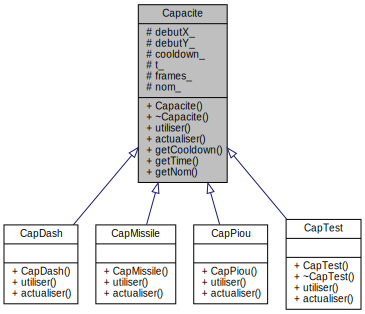
\includegraphics[width=282pt]{class_capacite__inherit__graph}
\end{center}
\end{figure}
\subsection*{Fonctions membres publiques}
\begin{DoxyCompactItemize}
\item 
\hyperlink{class_capacite_a8a1aebc5b2332e366a3f207c23b4d363}{Capacite} ()=default
\begin{DoxyCompactList}\small\item\em Constructeur. \end{DoxyCompactList}\item 
virtual \hyperlink{class_capacite_a43be1570a24a64682ff3f034330779a9}{$\sim$\+Capacite} ()=default
\begin{DoxyCompactList}\small\item\em Destructeur. \end{DoxyCompactList}\item 
virtual void \hyperlink{class_capacite_a6f5e6efda11f80ab8538e23f5bdc6e79}{utiliser} (int x, int y)=0
\begin{DoxyCompactList}\small\item\em Fonction virtuel qui active la capacite lorsqu\textquotesingle{}elle est appelée. \end{DoxyCompactList}\item 
virtual void \hyperlink{class_capacite_a924214972f385ef409031bafc0f315b7}{actualiser} (std\+::vector$<$ \hyperlink{class_projectile}{Projectile} $\ast$$>$ \&projectiles, \hyperlink{class_entite}{Entite} $\ast$vaisseau, float temps\+Ecoule)=0
\begin{DoxyCompactList}\small\item\em Fonction virtuel qui active les effets de la capacité \end{DoxyCompactList}\item 
float const \hyperlink{class_capacite_af07c1c3a2c9259a7eab270b3d8f867de}{get\+Cooldown} ()
\item 
float const \hyperlink{class_capacite_a963dd214cc53c76358b5326d9164884f}{get\+Time} ()
\item 
std\+::string const \hyperlink{class_capacite_a96218b289768ff461ffaaa0abe014a42}{get\+Nom} ()
\end{DoxyCompactItemize}
\subsection*{Attributs protégés}
\begin{DoxyCompactItemize}
\item 
int \hyperlink{class_capacite_abc3eb04129009107c0b60b03e7a3ff06}{debut\+X\+\_\+}
\item 
int \hyperlink{class_capacite_a741d48934a015c226b15e6519724e400}{debut\+Y\+\_\+}
\item 
float \hyperlink{class_capacite_aa84204be03602333d694faa14dbb693c}{cooldown\+\_\+}
\begin{DoxyCompactList}\small\item\em Position de départ. \end{DoxyCompactList}\item 
float \hyperlink{class_capacite_ade805898750e70261be4f4ced92a9063}{t\+\_\+}
\begin{DoxyCompactList}\small\item\em Temps à attendre avant de pouvoir utiliser la capacité à nouveau. \end{DoxyCompactList}\item 
unsigned int \hyperlink{class_capacite_a250c28dafd8e12b58ccfb4224329f111}{frames\+\_\+}
\begin{DoxyCompactList}\small\item\em Temps écoulé depuis la dernière activation de la compétance. \end{DoxyCompactList}\item 
std\+::string \hyperlink{class_capacite_a430472b509233086cbad1d6d8332dc8c}{nom\+\_\+}
\begin{DoxyCompactList}\small\item\em Nombre de frames écoulé depuis la dernière activation. \end{DoxyCompactList}\end{DoxyCompactItemize}


\subsection{Description détaillée}
Classe abstraite qui définit la structure générale d\textquotesingle{}une capacité, à faire hériter de chaque capacité 

Cette classe abstraite permet de définir la structure générale d\textquotesingle{}une capacité du jeu, elle doit être héritée pour chaque capacité qui est ajoutée au jeu 

\subsection{Documentation des constructeurs et destructeur}
\mbox{\Hypertarget{class_capacite_a8a1aebc5b2332e366a3f207c23b4d363}\label{class_capacite_a8a1aebc5b2332e366a3f207c23b4d363}} 
\index{Capacite@{Capacite}!Capacite@{Capacite}}
\index{Capacite@{Capacite}!Capacite@{Capacite}}
\subsubsection{\texorpdfstring{Capacite()}{Capacite()}}
{\footnotesize\ttfamily Capacite\+::\+Capacite (\begin{DoxyParamCaption}{ }\end{DoxyParamCaption})\hspace{0.3cm}{\ttfamily [default]}}



Constructeur. 

Vide \mbox{\Hypertarget{class_capacite_a43be1570a24a64682ff3f034330779a9}\label{class_capacite_a43be1570a24a64682ff3f034330779a9}} 
\index{Capacite@{Capacite}!````~Capacite@{$\sim$\+Capacite}}
\index{````~Capacite@{$\sim$\+Capacite}!Capacite@{Capacite}}
\subsubsection{\texorpdfstring{$\sim$\+Capacite()}{~Capacite()}}
{\footnotesize\ttfamily Capacite\+::$\sim$\+Capacite (\begin{DoxyParamCaption}{ }\end{DoxyParamCaption})\hspace{0.3cm}{\ttfamily [virtual]}, {\ttfamily [default]}}



Destructeur. 

Vide 

\subsection{Documentation des fonctions membres}
\mbox{\Hypertarget{class_capacite_a924214972f385ef409031bafc0f315b7}\label{class_capacite_a924214972f385ef409031bafc0f315b7}} 
\index{Capacite@{Capacite}!actualiser@{actualiser}}
\index{actualiser@{actualiser}!Capacite@{Capacite}}
\subsubsection{\texorpdfstring{actualiser()}{actualiser()}}
{\footnotesize\ttfamily Capacite\+::actualiser (\begin{DoxyParamCaption}\item[{std\+::vector$<$ \hyperlink{class_projectile}{Projectile} $\ast$$>$ \&}]{projectiles,  }\item[{\hyperlink{class_entite}{Entite} $\ast$}]{vaisseau,  }\item[{float}]{temps\+Ecoule }\end{DoxyParamCaption})\hspace{0.3cm}{\ttfamily [pure virtual]}}



Fonction virtuel qui active les effets de la capacité 


\begin{DoxyParams}{Paramètres}
{\em projectile} & Vecteur de tout les projectiles présent à l\textquotesingle{}écran \\
\hline
{\em vaisseau} & \hyperlink{class_vaisseau}{Vaisseau} qui a activé la compétance \\
\hline
{\em temp\+Ecoule} & Temps écoulé depuis la dernière boucle\\
\hline
\end{DoxyParams}
Fonction virtuel qui gère la création de projectiles et des modifications à apporter au vaisseau 

Implémenté dans \hyperlink{class_cap_piou_ae15af0a5a261349ae8462f00b6cb0d5d}{Cap\+Piou}, \hyperlink{class_cap_dash_ad4f99cef49151c1072a11af18852fa7b}{Cap\+Dash}, et \hyperlink{class_cap_test_af8e8fad88e1e4f0037eee576331d3238}{Cap\+Test}.

\mbox{\Hypertarget{class_capacite_af07c1c3a2c9259a7eab270b3d8f867de}\label{class_capacite_af07c1c3a2c9259a7eab270b3d8f867de}} 
\index{Capacite@{Capacite}!get\+Cooldown@{get\+Cooldown}}
\index{get\+Cooldown@{get\+Cooldown}!Capacite@{Capacite}}
\subsubsection{\texorpdfstring{get\+Cooldown()}{getCooldown()}}
{\footnotesize\ttfamily float const Capacite\+::get\+Cooldown (\begin{DoxyParamCaption}{ }\end{DoxyParamCaption})\hspace{0.3cm}{\ttfamily [inline]}}

\mbox{\Hypertarget{class_capacite_a96218b289768ff461ffaaa0abe014a42}\label{class_capacite_a96218b289768ff461ffaaa0abe014a42}} 
\index{Capacite@{Capacite}!get\+Nom@{get\+Nom}}
\index{get\+Nom@{get\+Nom}!Capacite@{Capacite}}
\subsubsection{\texorpdfstring{get\+Nom()}{getNom()}}
{\footnotesize\ttfamily std\+::string const Capacite\+::get\+Nom (\begin{DoxyParamCaption}{ }\end{DoxyParamCaption})\hspace{0.3cm}{\ttfamily [inline]}}

\mbox{\Hypertarget{class_capacite_a963dd214cc53c76358b5326d9164884f}\label{class_capacite_a963dd214cc53c76358b5326d9164884f}} 
\index{Capacite@{Capacite}!get\+Time@{get\+Time}}
\index{get\+Time@{get\+Time}!Capacite@{Capacite}}
\subsubsection{\texorpdfstring{get\+Time()}{getTime()}}
{\footnotesize\ttfamily float const Capacite\+::get\+Time (\begin{DoxyParamCaption}{ }\end{DoxyParamCaption})\hspace{0.3cm}{\ttfamily [inline]}}

\mbox{\Hypertarget{class_capacite_a6f5e6efda11f80ab8538e23f5bdc6e79}\label{class_capacite_a6f5e6efda11f80ab8538e23f5bdc6e79}} 
\index{Capacite@{Capacite}!utiliser@{utiliser}}
\index{utiliser@{utiliser}!Capacite@{Capacite}}
\subsubsection{\texorpdfstring{utiliser()}{utiliser()}}
{\footnotesize\ttfamily Capacite\+::utiliser (\begin{DoxyParamCaption}\item[{int}]{x,  }\item[{int}]{y }\end{DoxyParamCaption})\hspace{0.3cm}{\ttfamily [pure virtual]}}



Fonction virtuel qui active la capacite lorsqu\textquotesingle{}elle est appelée. 


\begin{DoxyParams}{Paramètres}
{\em x} & Abscisse de la postion où la capacite est utilisée \\
\hline
{\em y} & Ordonnée de la postion où la capacite est utilisée\\
\hline
\end{DoxyParams}
Fonction virtuel qui initialise la postion de départ et le timer 

Implémenté dans \hyperlink{class_cap_piou_a92f5cc3011280ad13bf3ff5e6a3c76ea}{Cap\+Piou}, \hyperlink{class_cap_dash_a82823122659ff5a87a09e9ddf0e3dabb}{Cap\+Dash}, et \hyperlink{class_cap_test_a9c85a17dec6cf78f1438b08b175f650d}{Cap\+Test}.



\subsection{Documentation des données membres}
\mbox{\Hypertarget{class_capacite_aa84204be03602333d694faa14dbb693c}\label{class_capacite_aa84204be03602333d694faa14dbb693c}} 
\index{Capacite@{Capacite}!cooldown\+\_\+@{cooldown\+\_\+}}
\index{cooldown\+\_\+@{cooldown\+\_\+}!Capacite@{Capacite}}
\subsubsection{\texorpdfstring{cooldown\+\_\+}{cooldown\_}}
{\footnotesize\ttfamily float Capacite\+::cooldown\+\_\+\hspace{0.3cm}{\ttfamily [protected]}}



Position de départ. 

\mbox{\Hypertarget{class_capacite_abc3eb04129009107c0b60b03e7a3ff06}\label{class_capacite_abc3eb04129009107c0b60b03e7a3ff06}} 
\index{Capacite@{Capacite}!debut\+X\+\_\+@{debut\+X\+\_\+}}
\index{debut\+X\+\_\+@{debut\+X\+\_\+}!Capacite@{Capacite}}
\subsubsection{\texorpdfstring{debut\+X\+\_\+}{debutX\_}}
{\footnotesize\ttfamily int Capacite\+::debut\+X\+\_\+\hspace{0.3cm}{\ttfamily [protected]}}

\mbox{\Hypertarget{class_capacite_a741d48934a015c226b15e6519724e400}\label{class_capacite_a741d48934a015c226b15e6519724e400}} 
\index{Capacite@{Capacite}!debut\+Y\+\_\+@{debut\+Y\+\_\+}}
\index{debut\+Y\+\_\+@{debut\+Y\+\_\+}!Capacite@{Capacite}}
\subsubsection{\texorpdfstring{debut\+Y\+\_\+}{debutY\_}}
{\footnotesize\ttfamily int Capacite\+::debut\+Y\+\_\+\hspace{0.3cm}{\ttfamily [protected]}}

\mbox{\Hypertarget{class_capacite_a250c28dafd8e12b58ccfb4224329f111}\label{class_capacite_a250c28dafd8e12b58ccfb4224329f111}} 
\index{Capacite@{Capacite}!frames\+\_\+@{frames\+\_\+}}
\index{frames\+\_\+@{frames\+\_\+}!Capacite@{Capacite}}
\subsubsection{\texorpdfstring{frames\+\_\+}{frames\_}}
{\footnotesize\ttfamily unsigned int Capacite\+::frames\+\_\+\hspace{0.3cm}{\ttfamily [protected]}}



Temps écoulé depuis la dernière activation de la compétance. 

\mbox{\Hypertarget{class_capacite_a430472b509233086cbad1d6d8332dc8c}\label{class_capacite_a430472b509233086cbad1d6d8332dc8c}} 
\index{Capacite@{Capacite}!nom\+\_\+@{nom\+\_\+}}
\index{nom\+\_\+@{nom\+\_\+}!Capacite@{Capacite}}
\subsubsection{\texorpdfstring{nom\+\_\+}{nom\_}}
{\footnotesize\ttfamily std\+::string Capacite\+::nom\+\_\+\hspace{0.3cm}{\ttfamily [protected]}}



Nombre de frames écoulé depuis la dernière activation. 

\mbox{\Hypertarget{class_capacite_ade805898750e70261be4f4ced92a9063}\label{class_capacite_ade805898750e70261be4f4ced92a9063}} 
\index{Capacite@{Capacite}!t\+\_\+@{t\+\_\+}}
\index{t\+\_\+@{t\+\_\+}!Capacite@{Capacite}}
\subsubsection{\texorpdfstring{t\+\_\+}{t\_}}
{\footnotesize\ttfamily float Capacite\+::t\+\_\+\hspace{0.3cm}{\ttfamily [protected]}}



Temps à attendre avant de pouvoir utiliser la capacité à nouveau. 



La documentation de cette classe a été générée à partir du fichier suivant \+:\begin{DoxyCompactItemize}
\item 
src/\+Capacites/\hyperlink{_capacite_8h}{Capacite.\+h}\end{DoxyCompactItemize}

\hypertarget{class_cap_dash}{}\section{Référence de la classe Cap\+Dash}
\label{class_cap_dash}\index{Cap\+Dash@{Cap\+Dash}}


{\ttfamily \#include $<$Cap\+Dash.\+h$>$}



Graphe d\textquotesingle{}héritage de Cap\+Dash\+:
\nopagebreak
\begin{figure}[H]
\begin{center}
\leavevmode
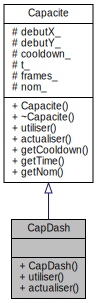
\includegraphics[width=138pt]{class_cap_dash__inherit__graph}
\end{center}
\end{figure}


Graphe de collaboration de Cap\+Dash\+:
\nopagebreak
\begin{figure}[H]
\begin{center}
\leavevmode
\includegraphics[width=138pt]{class_cap_dash__coll__graph}
\end{center}
\end{figure}
\subsection*{Fonctions membres publiques}
\begin{DoxyCompactItemize}
\item 
\hyperlink{class_cap_dash_ac38287e31284b6b5ac8add730830bfed}{Cap\+Dash} ()
\item 
\hyperlink{class_cap_dash_aa935262b9ebdaf197294aba7211663cc}{$\sim$\+Cap\+Dash} ()
\item 
void \hyperlink{class_cap_dash_ada59ecb62d2c18f6bb6b4acf28a2da93}{utiliser} (int x, int y)
\item 
void \hyperlink{class_cap_dash_a886522c648db49b81c330737ad96a517}{actualiser} (std\+::vector$<$ \hyperlink{class_projectile}{Projectile} $\ast$$>$ \&projectiles, \hyperlink{class_entite}{Entite} $\ast$vaisseau)
\end{DoxyCompactItemize}
\subsection*{Membres hérités additionnels}


\subsection{Documentation des constructeurs et destructeur}
\mbox{\Hypertarget{class_cap_dash_ac38287e31284b6b5ac8add730830bfed}\label{class_cap_dash_ac38287e31284b6b5ac8add730830bfed}} 
\index{Cap\+Dash@{Cap\+Dash}!Cap\+Dash@{Cap\+Dash}}
\index{Cap\+Dash@{Cap\+Dash}!Cap\+Dash@{Cap\+Dash}}
\subsubsection{\texorpdfstring{Cap\+Dash()}{CapDash()}}
{\footnotesize\ttfamily Cap\+Dash\+::\+Cap\+Dash (\begin{DoxyParamCaption}{ }\end{DoxyParamCaption})}

\mbox{\Hypertarget{class_cap_dash_aa935262b9ebdaf197294aba7211663cc}\label{class_cap_dash_aa935262b9ebdaf197294aba7211663cc}} 
\index{Cap\+Dash@{Cap\+Dash}!````~Cap\+Dash@{$\sim$\+Cap\+Dash}}
\index{````~Cap\+Dash@{$\sim$\+Cap\+Dash}!Cap\+Dash@{Cap\+Dash}}
\subsubsection{\texorpdfstring{$\sim$\+Cap\+Dash()}{~CapDash()}}
{\footnotesize\ttfamily Cap\+Dash\+::$\sim$\+Cap\+Dash (\begin{DoxyParamCaption}{ }\end{DoxyParamCaption})}



\subsection{Documentation des fonctions membres}
\mbox{\Hypertarget{class_cap_dash_a886522c648db49b81c330737ad96a517}\label{class_cap_dash_a886522c648db49b81c330737ad96a517}} 
\index{Cap\+Dash@{Cap\+Dash}!actualiser@{actualiser}}
\index{actualiser@{actualiser}!Cap\+Dash@{Cap\+Dash}}
\subsubsection{\texorpdfstring{actualiser()}{actualiser()}}
{\footnotesize\ttfamily void Cap\+Dash\+::actualiser (\begin{DoxyParamCaption}\item[{std\+::vector$<$ \hyperlink{class_projectile}{Projectile} $\ast$$>$ \&}]{projectiles,  }\item[{\hyperlink{class_entite}{Entite} $\ast$}]{vaisseau }\end{DoxyParamCaption})\hspace{0.3cm}{\ttfamily [virtual]}}



Implémente \hyperlink{class_capacite_a7d4e86c20cd198960f25c0eb443148fe}{Capacite}.

\mbox{\Hypertarget{class_cap_dash_ada59ecb62d2c18f6bb6b4acf28a2da93}\label{class_cap_dash_ada59ecb62d2c18f6bb6b4acf28a2da93}} 
\index{Cap\+Dash@{Cap\+Dash}!utiliser@{utiliser}}
\index{utiliser@{utiliser}!Cap\+Dash@{Cap\+Dash}}
\subsubsection{\texorpdfstring{utiliser()}{utiliser()}}
{\footnotesize\ttfamily void Cap\+Dash\+::utiliser (\begin{DoxyParamCaption}\item[{int}]{x,  }\item[{int}]{y }\end{DoxyParamCaption})\hspace{0.3cm}{\ttfamily [virtual]}}



Implémente \hyperlink{class_capacite_a4d4f643987fcc2168567bf28a36ea418}{Capacite}.



La documentation de cette classe a été générée à partir des fichiers suivants \+:\begin{DoxyCompactItemize}
\item 
src/\+Capacites/\hyperlink{_cap_dash_8h}{Cap\+Dash.\+h}\item 
src/\+Capacites/\hyperlink{_cap_dash_8cpp}{Cap\+Dash.\+cpp}\end{DoxyCompactItemize}

\hypertarget{class_cap_piou}{}\section{Référence de la classe Cap\+Piou}
\label{class_cap_piou}\index{Cap\+Piou@{Cap\+Piou}}


{\ttfamily \#include $<$Cap\+Piou.\+h$>$}



Graphe d\textquotesingle{}héritage de Cap\+Piou\+:\nopagebreak
\begin{figure}[H]
\begin{center}
\leavevmode
\includegraphics[width=136pt]{class_cap_piou__inherit__graph}
\end{center}
\end{figure}


Graphe de collaboration de Cap\+Piou\+:\nopagebreak
\begin{figure}[H]
\begin{center}
\leavevmode
\includegraphics[width=136pt]{class_cap_piou__coll__graph}
\end{center}
\end{figure}
\subsection*{Fonctions membres publiques}
\begin{DoxyCompactItemize}
\item 
\hyperlink{class_cap_piou_aa2ed61fb1313a447cf8444399001750d}{Cap\+Piou} ()
\item 
\hyperlink{class_cap_piou_a35d7e0b0c14d6a6e01ba0a053a8a60bd}{$\sim$\+Cap\+Piou} ()
\item 
void \hyperlink{class_cap_piou_a20ed7a993ce209a3df246f655f107f22}{utiliser} (int x, int y)
\item 
void \hyperlink{class_cap_piou_aabdcaa253f10db2bca12e750005485fc}{actualiser} (std\+::vector$<$ \hyperlink{class_projectile}{Projectile} $\ast$$>$ \&projectiles, \hyperlink{class_entite}{Entite} $\ast$vaisseau)
\end{DoxyCompactItemize}
\subsection*{Membres hérités additionnels}


\subsection{Documentation des constructeurs et destructeur}
\mbox{\Hypertarget{class_cap_piou_aa2ed61fb1313a447cf8444399001750d}\label{class_cap_piou_aa2ed61fb1313a447cf8444399001750d}} 
\index{Cap\+Piou@{Cap\+Piou}!Cap\+Piou@{Cap\+Piou}}
\index{Cap\+Piou@{Cap\+Piou}!Cap\+Piou@{Cap\+Piou}}
\subsubsection{\texorpdfstring{Cap\+Piou()}{CapPiou()}}
{\footnotesize\ttfamily Cap\+Piou\+::\+Cap\+Piou (\begin{DoxyParamCaption}{ }\end{DoxyParamCaption})}

\mbox{\Hypertarget{class_cap_piou_a35d7e0b0c14d6a6e01ba0a053a8a60bd}\label{class_cap_piou_a35d7e0b0c14d6a6e01ba0a053a8a60bd}} 
\index{Cap\+Piou@{Cap\+Piou}!````~Cap\+Piou@{$\sim$\+Cap\+Piou}}
\index{````~Cap\+Piou@{$\sim$\+Cap\+Piou}!Cap\+Piou@{Cap\+Piou}}
\subsubsection{\texorpdfstring{$\sim$\+Cap\+Piou()}{~CapPiou()}}
{\footnotesize\ttfamily Cap\+Piou\+::$\sim$\+Cap\+Piou (\begin{DoxyParamCaption}{ }\end{DoxyParamCaption})}



\subsection{Documentation des fonctions membres}
\mbox{\Hypertarget{class_cap_piou_aabdcaa253f10db2bca12e750005485fc}\label{class_cap_piou_aabdcaa253f10db2bca12e750005485fc}} 
\index{Cap\+Piou@{Cap\+Piou}!actualiser@{actualiser}}
\index{actualiser@{actualiser}!Cap\+Piou@{Cap\+Piou}}
\subsubsection{\texorpdfstring{actualiser()}{actualiser()}}
{\footnotesize\ttfamily void Cap\+Piou\+::actualiser (\begin{DoxyParamCaption}\item[{std\+::vector$<$ \hyperlink{class_projectile}{Projectile} $\ast$$>$ \&}]{projectiles,  }\item[{\hyperlink{class_entite}{Entite} $\ast$}]{vaisseau }\end{DoxyParamCaption})\hspace{0.3cm}{\ttfamily [virtual]}}



Implémente \hyperlink{class_capacite_a7d4e86c20cd198960f25c0eb443148fe}{Capacite}.

\mbox{\Hypertarget{class_cap_piou_a20ed7a993ce209a3df246f655f107f22}\label{class_cap_piou_a20ed7a993ce209a3df246f655f107f22}} 
\index{Cap\+Piou@{Cap\+Piou}!utiliser@{utiliser}}
\index{utiliser@{utiliser}!Cap\+Piou@{Cap\+Piou}}
\subsubsection{\texorpdfstring{utiliser()}{utiliser()}}
{\footnotesize\ttfamily void Cap\+Piou\+::utiliser (\begin{DoxyParamCaption}\item[{int}]{x,  }\item[{int}]{y }\end{DoxyParamCaption})\hspace{0.3cm}{\ttfamily [virtual]}}



Implémente \hyperlink{class_capacite_a4d4f643987fcc2168567bf28a36ea418}{Capacite}.



La documentation de cette classe a été générée à partir des fichiers suivants \+:\begin{DoxyCompactItemize}
\item 
src/\+Capacites/\hyperlink{_cap_piou_8h}{Cap\+Piou.\+h}\item 
src/\+Capacites/\hyperlink{_cap_piou_8cpp}{Cap\+Piou.\+cpp}\end{DoxyCompactItemize}

\hypertarget{class_cap_test}{}\section{Référence de la classe Cap\+Test}
\label{class_cap_test}\index{Cap\+Test@{Cap\+Test}}


{\ttfamily \#include $<$Cap\+Test.\+h$>$}



Graphe d\textquotesingle{}héritage de Cap\+Test\+:\nopagebreak
\begin{figure}[H]
\begin{center}
\leavevmode
\includegraphics[width=136pt]{class_cap_test__inherit__graph}
\end{center}
\end{figure}


Graphe de collaboration de Cap\+Test\+:\nopagebreak
\begin{figure}[H]
\begin{center}
\leavevmode
\includegraphics[width=136pt]{class_cap_test__coll__graph}
\end{center}
\end{figure}
\subsection*{Fonctions membres publiques}
\begin{DoxyCompactItemize}
\item 
\hyperlink{class_cap_test_a5f6d4b172a6a40f974b3f7414e3f06e5}{Cap\+Test} ()
\item 
\hyperlink{class_cap_test_a92687aa212347d1738e7736cb107d03b}{$\sim$\+Cap\+Test} ()
\item 
void \hyperlink{class_cap_test_af85984f6d9330e5527feff1a62ee4242}{utiliser} (int x, int y)
\item 
void \hyperlink{class_cap_test_a5742770894ff765e2785f82aab88b223}{actualiser} (std\+::vector$<$ \hyperlink{class_projectile}{Projectile} $\ast$$>$ \&projectiles, \hyperlink{class_entite}{Entite} $\ast$vaisseau)
\end{DoxyCompactItemize}
\subsection*{Membres hérités additionnels}


\subsection{Documentation des constructeurs et destructeur}
\mbox{\Hypertarget{class_cap_test_a5f6d4b172a6a40f974b3f7414e3f06e5}\label{class_cap_test_a5f6d4b172a6a40f974b3f7414e3f06e5}} 
\index{Cap\+Test@{Cap\+Test}!Cap\+Test@{Cap\+Test}}
\index{Cap\+Test@{Cap\+Test}!Cap\+Test@{Cap\+Test}}
\subsubsection{\texorpdfstring{Cap\+Test()}{CapTest()}}
{\footnotesize\ttfamily Cap\+Test\+::\+Cap\+Test (\begin{DoxyParamCaption}{ }\end{DoxyParamCaption})}

\mbox{\Hypertarget{class_cap_test_a92687aa212347d1738e7736cb107d03b}\label{class_cap_test_a92687aa212347d1738e7736cb107d03b}} 
\index{Cap\+Test@{Cap\+Test}!````~Cap\+Test@{$\sim$\+Cap\+Test}}
\index{````~Cap\+Test@{$\sim$\+Cap\+Test}!Cap\+Test@{Cap\+Test}}
\subsubsection{\texorpdfstring{$\sim$\+Cap\+Test()}{~CapTest()}}
{\footnotesize\ttfamily Cap\+Test\+::$\sim$\+Cap\+Test (\begin{DoxyParamCaption}{ }\end{DoxyParamCaption})}



\subsection{Documentation des fonctions membres}
\mbox{\Hypertarget{class_cap_test_a5742770894ff765e2785f82aab88b223}\label{class_cap_test_a5742770894ff765e2785f82aab88b223}} 
\index{Cap\+Test@{Cap\+Test}!actualiser@{actualiser}}
\index{actualiser@{actualiser}!Cap\+Test@{Cap\+Test}}
\subsubsection{\texorpdfstring{actualiser()}{actualiser()}}
{\footnotesize\ttfamily void Cap\+Test\+::actualiser (\begin{DoxyParamCaption}\item[{std\+::vector$<$ \hyperlink{class_projectile}{Projectile} $\ast$$>$ \&}]{projectiles,  }\item[{\hyperlink{class_entite}{Entite} $\ast$}]{vaisseau }\end{DoxyParamCaption})\hspace{0.3cm}{\ttfamily [virtual]}}



Implémente \hyperlink{class_capacite_a7d4e86c20cd198960f25c0eb443148fe}{Capacite}.

\mbox{\Hypertarget{class_cap_test_af85984f6d9330e5527feff1a62ee4242}\label{class_cap_test_af85984f6d9330e5527feff1a62ee4242}} 
\index{Cap\+Test@{Cap\+Test}!utiliser@{utiliser}}
\index{utiliser@{utiliser}!Cap\+Test@{Cap\+Test}}
\subsubsection{\texorpdfstring{utiliser()}{utiliser()}}
{\footnotesize\ttfamily void Cap\+Test\+::utiliser (\begin{DoxyParamCaption}\item[{int}]{x,  }\item[{int}]{y }\end{DoxyParamCaption})\hspace{0.3cm}{\ttfamily [virtual]}}



Implémente \hyperlink{class_capacite_a4d4f643987fcc2168567bf28a36ea418}{Capacite}.



La documentation de cette classe a été générée à partir des fichiers suivants \+:\begin{DoxyCompactItemize}
\item 
src/\hyperlink{_cap_test_8h}{Cap\+Test.\+h}\item 
src/\hyperlink{_cap_test_8cpp}{Cap\+Test.\+cpp}\end{DoxyCompactItemize}

\hypertarget{class_entite}{}\section{Référence de la classe Entite}
\label{class_entite}\index{Entite@{Entite}}


Classe virtuelle qui définit une entité  




{\ttfamily \#include $<$Entite.\+h$>$}



Graphe d\textquotesingle{}héritage de Entite\+:\nopagebreak
\begin{figure}[H]
\begin{center}
\leavevmode
\includegraphics[width=299pt]{class_entite__inherit__graph}
\end{center}
\end{figure}
\subsection*{Fonctions membres publiques}
\begin{DoxyCompactItemize}
\item 
virtual \hyperlink{class_entite_a8084762a25afbfbcdca31121a3dfcd87}{$\sim$\+Entite} ()=default
\begin{DoxyCompactList}\small\item\em Destructeur par défaut. \end{DoxyCompactList}\item 
const std\+::vector$<$ std\+::unique\+\_\+ptr$<$ sf\+::\+Shape $>$ $>$ \& \hyperlink{class_entite_ae01177a102251100c96e2060372627ad}{get\+Forme} () const
\item 
void \hyperlink{class_entite_a91874d7e87f6cb479a3893fbedc6a4e3}{afficher} (sf\+::\+Render\+Window \&window, bool debug=false) const
\begin{DoxyCompactList}\small\item\em Affiche le sprite de l\textquotesingle{}\hyperlink{class_entite}{Entite}. \end{DoxyCompactList}\item 
void \hyperlink{class_entite_ac409613f3cf67cae14babd4b16811c8f}{move} (const sf\+::\+Vector2f \&delta)
\begin{DoxyCompactList}\small\item\em Déplace l\textquotesingle{}\hyperlink{class_entite}{Entite} en fonction de {\itshape delta}. \end{DoxyCompactList}\item 
void \hyperlink{class_entite_aa7fe4a7ebd8eb4c80ef9fdb7d97f2dad}{set\+Position} (const sf\+::\+Vector2f \&pos)
\begin{DoxyCompactList}\small\item\em Fixe la position de l\textquotesingle{}\hyperlink{class_entite}{Entite}. \end{DoxyCompactList}\item 
const sf\+::\+Vector2f \& \hyperlink{class_entite_a6f6fd1e1f9f6ad44f0ecc74961a774d9}{get\+Position} () const
\begin{DoxyCompactList}\small\item\em Renvoie la position de l\textquotesingle{}\hyperlink{class_entite}{Entite} appelante. \end{DoxyCompactList}\item 
void \hyperlink{class_entite_af1249039d313e4e691a109440663eae7}{rotate} (float angle)
\begin{DoxyCompactList}\small\item\em Tourne l\textquotesingle{}\hyperlink{class_entite}{Entite} de l\textquotesingle{}angle passé en paramètre. \end{DoxyCompactList}\item 
void \hyperlink{class_entite_a8623ac815e34b553098f45696ea8918b}{set\+Rotation} (float angle)
\begin{DoxyCompactList}\small\item\em Fixe l\textquotesingle{}orientation de l\textquotesingle{}\hyperlink{class_entite}{Entite} appelante. \end{DoxyCompactList}\item 
float \hyperlink{class_entite_a7f19439f7e7a5028f4b26eff21683de9}{get\+Rotation} () const
\begin{DoxyCompactList}\small\item\em Récupère l\textquotesingle{}orientation de l\textquotesingle{}\hyperlink{class_entite}{Entite}. \end{DoxyCompactList}\item 
void \hyperlink{class_entite_a770f6c53856606c4de768bb942299659}{scale} (float factor)
\begin{DoxyCompactList}\small\item\em Change l\textquotesingle{}échelle de l\textquotesingle{}\hyperlink{class_entite}{Entite}. \end{DoxyCompactList}\item 
void \hyperlink{class_entite_a665939253829baba965ce3ead0f1739c}{set\+Scale} (float factor)
\begin{DoxyCompactList}\small\item\em Fixer l\textquotesingle{}échelle de L\textquotesingle{}entite. \end{DoxyCompactList}\item 
float \hyperlink{class_entite_a5f70868f62049291edf4b245a531a6e0}{get\+Scale} () const
\begin{DoxyCompactList}\small\item\em Renvoie l\textquotesingle{}échelle de l\textquotesingle{}\hyperlink{class_entite}{Entite}. \end{DoxyCompactList}\item 
bool \hyperlink{class_entite_a8734ec47c87feb2b8b221bbf5d9ff2b4}{est\+Dehors} () const
\item 
void \hyperlink{class_entite_a88c148848289e34ca3bc991c37db9b44}{change\+Speed} (int val)
\end{DoxyCompactItemize}
\subsection*{Attributs protégés}
\begin{DoxyCompactItemize}
\item 
bool \hyperlink{class_entite_a37bb9bd568e9e1c904eaa83ec49a2b16}{collisionable\+\_\+} = true
\begin{DoxyCompactList}\small\item\em Booléen vrai si collisionnable. \end{DoxyCompactList}\item 
int \hyperlink{class_entite_a86f42758a3e4672052331b7a4daa10b5}{equipe\+\_\+}
\begin{DoxyCompactList}\small\item\em numéro d\textquotesingle{}équipe \end{DoxyCompactList}\item 
sf\+::\+Vector2f \hyperlink{class_entite_abbd554c4f122159a73cb113cc8de3860}{position\+\_\+}
\item 
float \hyperlink{class_entite_a2d6dc6bfcee492337b7422f12b393141}{angle\+\_\+}
\item 
float \hyperlink{class_entite_a50e0f8c1188d9833432c55c7f7d2aa0f}{scale\+\_\+}
\item 
sf\+::\+Circle\+Shape \hyperlink{class_entite_a5b6c62e4dc54221a84ce4dc824fdb2da}{cercle\+Englobant\+\_\+}
\item 
std\+::vector$<$ std\+::unique\+\_\+ptr$<$ sf\+::\+Shape $>$ $>$ \hyperlink{class_entite_aa6bbda9a40f701f273c344406a6f5122}{forme\+\_\+}
\item 
sf\+::\+Texture \hyperlink{class_entite_a8147b9459318a9b1de1b72dce115680a}{texture\+\_\+}
\item 
sf\+::\+Sprite \hyperlink{class_entite_ab7c03b6fe5c4f1d08cd3e4304e0ef7c0}{sprite\+\_\+}
\item 
int \hyperlink{class_entite_a62c3145096f707457d60306ea6729ed6}{vit\+\_\+}
\begin{DoxyCompactList}\small\item\em Vitesse actuelle. \end{DoxyCompactList}\end{DoxyCompactItemize}
\subsection*{Amis}
\begin{DoxyCompactItemize}
\item 
bool \hyperlink{class_entite_ac5011435e5099909dd34cd1750933b30}{collision} (const \hyperlink{class_entite}{Entite} \&e1, const \hyperlink{class_entite}{Entite} \&e2)
\begin{DoxyCompactList}\small\item\em Détecte une collision entre deux \hyperlink{class_entite}{Entite}. \end{DoxyCompactList}\end{DoxyCompactItemize}


\subsection{Description détaillée}
Classe virtuelle qui définit une entité 

Cette classe est une base à toutes les entités du jeu, les vaisseaux et les projectiles. Elle définit l\textquotesingle{}interface globale à travers laquelle ces entités peuvent être manipulées 

\subsection{Documentation des constructeurs et destructeur}
\mbox{\Hypertarget{class_entite_a8084762a25afbfbcdca31121a3dfcd87}\label{class_entite_a8084762a25afbfbcdca31121a3dfcd87}} 
\index{Entite@{Entite}!````~Entite@{$\sim$\+Entite}}
\index{````~Entite@{$\sim$\+Entite}!Entite@{Entite}}
\subsubsection{\texorpdfstring{$\sim$\+Entite()}{~Entite()}}
{\footnotesize\ttfamily Entite\+::$\sim$\+Entite (\begin{DoxyParamCaption}{ }\end{DoxyParamCaption})\hspace{0.3cm}{\ttfamily [virtual]}, {\ttfamily [default]}}



Destructeur par défaut. 

Destructeur virtuel par défaut de la classe \hyperlink{class_entite}{Entite}. Le destructeur est virtuel car la classe a vocation à être héritée. Il n\textquotesingle{}y a rien de spécial à faire donc le destructeur par défaut convient 

\subsection{Documentation des fonctions membres}
\mbox{\Hypertarget{class_entite_a91874d7e87f6cb479a3893fbedc6a4e3}\label{class_entite_a91874d7e87f6cb479a3893fbedc6a4e3}} 
\index{Entite@{Entite}!afficher@{afficher}}
\index{afficher@{afficher}!Entite@{Entite}}
\subsubsection{\texorpdfstring{afficher()}{afficher()}}
{\footnotesize\ttfamily Entite\+::afficher (\begin{DoxyParamCaption}\item[{sf\+::\+Render\+Window \&}]{window,  }\item[{bool}]{debug = {\ttfamily false} }\end{DoxyParamCaption}) const}



Affiche le sprite de l\textquotesingle{}\hyperlink{class_entite}{Entite}. 

Appelle la fonction afficher de la S\+F\+ML sur les attributs de l\textquotesingle{}objet appelant. Peut également afficher des informations de debug telles que le cercle englobant, et la forme de collision. 
\begin{DoxyParams}[1]{Paramètres}
\mbox{\tt in,out}  & {\em window} & Fenêtre S\+F\+ML dans laquelle afficher l\textquotesingle{}entité. \\
\hline
\mbox{\tt in}  & {\em debug} & Un {\ttfamily bool} qui vaut {\itshape true} si les informations de debug doivent être affichées et {\itshape false} sinon. \\
\hline
\end{DoxyParams}
\mbox{\Hypertarget{class_entite_a88c148848289e34ca3bc991c37db9b44}\label{class_entite_a88c148848289e34ca3bc991c37db9b44}} 
\index{Entite@{Entite}!change\+Speed@{change\+Speed}}
\index{change\+Speed@{change\+Speed}!Entite@{Entite}}
\subsubsection{\texorpdfstring{change\+Speed()}{changeSpeed()}}
{\footnotesize\ttfamily void Entite\+::change\+Speed (\begin{DoxyParamCaption}\item[{int}]{val }\end{DoxyParamCaption})}

\mbox{\Hypertarget{class_entite_a8734ec47c87feb2b8b221bbf5d9ff2b4}\label{class_entite_a8734ec47c87feb2b8b221bbf5d9ff2b4}} 
\index{Entite@{Entite}!est\+Dehors@{est\+Dehors}}
\index{est\+Dehors@{est\+Dehors}!Entite@{Entite}}
\subsubsection{\texorpdfstring{est\+Dehors()}{estDehors()}}
{\footnotesize\ttfamily bool Entite\+::est\+Dehors (\begin{DoxyParamCaption}{ }\end{DoxyParamCaption}) const}

\mbox{\Hypertarget{class_entite_ae01177a102251100c96e2060372627ad}\label{class_entite_ae01177a102251100c96e2060372627ad}} 
\index{Entite@{Entite}!get\+Forme@{get\+Forme}}
\index{get\+Forme@{get\+Forme}!Entite@{Entite}}
\subsubsection{\texorpdfstring{get\+Forme()}{getForme()}}
{\footnotesize\ttfamily const std\+::vector$<$std\+::unique\+\_\+ptr$<$sf\+::\+Shape$>$ $>$\& Entite\+::get\+Forme (\begin{DoxyParamCaption}{ }\end{DoxyParamCaption}) const\hspace{0.3cm}{\ttfamily [inline]}}

\mbox{\Hypertarget{class_entite_a6f6fd1e1f9f6ad44f0ecc74961a774d9}\label{class_entite_a6f6fd1e1f9f6ad44f0ecc74961a774d9}} 
\index{Entite@{Entite}!get\+Position@{get\+Position}}
\index{get\+Position@{get\+Position}!Entite@{Entite}}
\subsubsection{\texorpdfstring{get\+Position()}{getPosition()}}
{\footnotesize\ttfamily Entite\+::get\+Position (\begin{DoxyParamCaption}{ }\end{DoxyParamCaption}) const}



Renvoie la position de l\textquotesingle{}\hyperlink{class_entite}{Entite} appelante. 

Cette fonction renvoie la position actuelle de l\textquotesingle{}\hyperlink{class_entite}{Entite} appelante par rapport au point haut gauche de la fenêtre \begin{DoxyReturn}{Renvoie}
la position de l\textquotesingle{}entité appelante 
\end{DoxyReturn}
\mbox{\Hypertarget{class_entite_a7f19439f7e7a5028f4b26eff21683de9}\label{class_entite_a7f19439f7e7a5028f4b26eff21683de9}} 
\index{Entite@{Entite}!get\+Rotation@{get\+Rotation}}
\index{get\+Rotation@{get\+Rotation}!Entite@{Entite}}
\subsubsection{\texorpdfstring{get\+Rotation()}{getRotation()}}
{\footnotesize\ttfamily Entite\+::get\+Rotation (\begin{DoxyParamCaption}{ }\end{DoxyParamCaption}) const}



Récupère l\textquotesingle{}orientation de l\textquotesingle{}\hyperlink{class_entite}{Entite}. 

Cette fonction renvoie l\textquotesingle{}orientation actuelle de l\textquotesingle{}\hyperlink{class_entite}{Entite} appelante. La valeur renvoyée correspond à un angle en degrés \begin{DoxyReturn}{Renvoie}
Un {\ttfamily float} qui correspond à l\textquotesingle{}eorientation de l\textquotesingle{}\hyperlink{class_entite}{Entite} 
\end{DoxyReturn}
\mbox{\Hypertarget{class_entite_a5f70868f62049291edf4b245a531a6e0}\label{class_entite_a5f70868f62049291edf4b245a531a6e0}} 
\index{Entite@{Entite}!get\+Scale@{get\+Scale}}
\index{get\+Scale@{get\+Scale}!Entite@{Entite}}
\subsubsection{\texorpdfstring{get\+Scale()}{getScale()}}
{\footnotesize\ttfamily Entite\+::get\+Scale (\begin{DoxyParamCaption}{ }\end{DoxyParamCaption}) const}



Renvoie l\textquotesingle{}échelle de l\textquotesingle{}\hyperlink{class_entite}{Entite}. 

Cette fonction renvoie l\textquotesingle{}échelle actuelle de l\textquotesingle{}\hyperlink{class_entite}{Entite} appelante \begin{DoxyReturn}{Renvoie}
Un {\ttfamily float} qui correspond au facteur d\textquotesingle{}échelle de l\textquotesingle{}\hyperlink{class_entite}{Entite} 
\end{DoxyReturn}
\mbox{\Hypertarget{class_entite_ac409613f3cf67cae14babd4b16811c8f}\label{class_entite_ac409613f3cf67cae14babd4b16811c8f}} 
\index{Entite@{Entite}!move@{move}}
\index{move@{move}!Entite@{Entite}}
\subsubsection{\texorpdfstring{move()}{move()}}
{\footnotesize\ttfamily Entite\+::move (\begin{DoxyParamCaption}\item[{const sf\+::\+Vector2f \&}]{delta }\end{DoxyParamCaption})}



Déplace l\textquotesingle{}\hyperlink{class_entite}{Entite} en fonction de {\itshape delta}. 

Appelle la fonction move de la S\+F\+ML sur les attributs de l\textquotesingle{}objet appelant. 
\begin{DoxyParams}[1]{Paramètres}
\mbox{\tt in}  & {\em delta} & un {\ttfamily sf\+::\+Vector2f} qui donne le déplacement en x et en y \\
\hline
\end{DoxyParams}
\mbox{\Hypertarget{class_entite_af1249039d313e4e691a109440663eae7}\label{class_entite_af1249039d313e4e691a109440663eae7}} 
\index{Entite@{Entite}!rotate@{rotate}}
\index{rotate@{rotate}!Entite@{Entite}}
\subsubsection{\texorpdfstring{rotate()}{rotate()}}
{\footnotesize\ttfamily Entite\+::rotate (\begin{DoxyParamCaption}\item[{float}]{angle }\end{DoxyParamCaption})}



Tourne l\textquotesingle{}\hyperlink{class_entite}{Entite} de l\textquotesingle{}angle passé en paramètre. 

Cette fonction permet de aire tourner l\textquotesingle{}entité de l\textquotesingle{}angle passé en paramètre, chaque élément composant l\textquotesingle{}entité est tourné. L\textquotesingle{}angle est donné en degrés 
\begin{DoxyParams}[1]{Paramètres}
\mbox{\tt in}  & {\em angle} & \\
\hline
\end{DoxyParams}
\mbox{\Hypertarget{class_entite_a770f6c53856606c4de768bb942299659}\label{class_entite_a770f6c53856606c4de768bb942299659}} 
\index{Entite@{Entite}!scale@{scale}}
\index{scale@{scale}!Entite@{Entite}}
\subsubsection{\texorpdfstring{scale()}{scale()}}
{\footnotesize\ttfamily Entite\+::scale (\begin{DoxyParamCaption}\item[{float}]{factor }\end{DoxyParamCaption})}



Change l\textquotesingle{}échelle de l\textquotesingle{}\hyperlink{class_entite}{Entite}. 

Cette fonction permet de modifier l\textquotesingle{}échelle de l\textquotesingle{}\hyperlink{class_entite}{Entite} appelante en appliquant un coefficient multiplicateur à ses dimensions. Un coefficient de 0.\+5 divisera les dimentions par 2, à l\textquotesingle{}inverse un coefficient de 2 rendra l\textquotesingle{}\hyperlink{class_entite}{Entite} 2 fois plus grande. Un coefficient de 1 ne changera rien. 
\begin{DoxyParams}[1]{Paramètres}
\mbox{\tt in}  & {\em factor} & Le coefficient multiplicateur d\textquotesingle{}échelle à appliquer \\
\hline
\end{DoxyParams}
\mbox{\Hypertarget{class_entite_aa7fe4a7ebd8eb4c80ef9fdb7d97f2dad}\label{class_entite_aa7fe4a7ebd8eb4c80ef9fdb7d97f2dad}} 
\index{Entite@{Entite}!set\+Position@{set\+Position}}
\index{set\+Position@{set\+Position}!Entite@{Entite}}
\subsubsection{\texorpdfstring{set\+Position()}{setPosition()}}
{\footnotesize\ttfamily Entite\+::set\+Position (\begin{DoxyParamCaption}\item[{const sf\+::\+Vector2f \&}]{pos }\end{DoxyParamCaption})}



Fixe la position de l\textquotesingle{}\hyperlink{class_entite}{Entite}. 

Cette fonction change la position de l\textquotesingle{}\hyperlink{class_entite}{Entite} appelante avec les coordonnées données en paramètres. Ces coordonnées sont relatives au coin supérieur gauche de la fenêtre. Cette fonction est implémentée à partir de la fonction {\itshape move} afin que chaque élément reste au même endroit par rapport aux autres s\textquotesingle{}il n\textquotesingle{}ont pas la même position initiale. 
\begin{DoxyParams}[1]{Paramètres}
\mbox{\tt in}  & {\em pos} & Un {\ttfamily sf\+::\+Vector2f} qui contient la nouvelle position \\
\hline
\end{DoxyParams}
\mbox{\Hypertarget{class_entite_a8623ac815e34b553098f45696ea8918b}\label{class_entite_a8623ac815e34b553098f45696ea8918b}} 
\index{Entite@{Entite}!set\+Rotation@{set\+Rotation}}
\index{set\+Rotation@{set\+Rotation}!Entite@{Entite}}
\subsubsection{\texorpdfstring{set\+Rotation()}{setRotation()}}
{\footnotesize\ttfamily Entite\+::set\+Rotation (\begin{DoxyParamCaption}\item[{float}]{angle }\end{DoxyParamCaption})}



Fixe l\textquotesingle{}orientation de l\textquotesingle{}\hyperlink{class_entite}{Entite} appelante. 

Cette fonction change l\textquotesingle{}orientation de l\textquotesingle{}\hyperlink{class_entite}{Entite} appelante à l\textquotesingle{}angle passé en paramètres. La valeur de l\textquotesingle{}angle est donnée en degrés. Cette fonction est implémentée en utilisant la fonction rotate pour que les éléments ne soient pa décalés les uns par rapport aux autres s\textquotesingle{}ils ne disposent pas de la même orientation initiale. 
\begin{DoxyParams}[1]{Paramètres}
\mbox{\tt in}  & {\em angle} & La nouvelle orientation de l\textquotesingle{}\hyperlink{class_entite}{Entite} \\
\hline
\end{DoxyParams}
\mbox{\Hypertarget{class_entite_a665939253829baba965ce3ead0f1739c}\label{class_entite_a665939253829baba965ce3ead0f1739c}} 
\index{Entite@{Entite}!set\+Scale@{set\+Scale}}
\index{set\+Scale@{set\+Scale}!Entite@{Entite}}
\subsubsection{\texorpdfstring{set\+Scale()}{setScale()}}
{\footnotesize\ttfamily Entite\+::set\+Scale (\begin{DoxyParamCaption}\item[{float}]{factor }\end{DoxyParamCaption})}



Fixer l\textquotesingle{}échelle de L\textquotesingle{}entite. 

Cette fonction permet de fixer l\textquotesingle{}échelle de L\textquotesingle{}entite appelante. Contrairement à la fonction scale, cette fonction fixe l\textquotesingle{}échelle de manière absolue et non relativement au changements d\textquotesingle{}échelle déjà appliqué à l\textquotesingle{}\hyperlink{class_entite}{Entite} 
\begin{DoxyParams}[1]{Paramètres}
\mbox{\tt in}  & {\em factor} & Le facteur d\textquotesingle{}échelle à appliquer \\
\hline
\end{DoxyParams}


\subsection{Documentation des fonctions amies et associées}
\mbox{\Hypertarget{class_entite_ac5011435e5099909dd34cd1750933b30}\label{class_entite_ac5011435e5099909dd34cd1750933b30}} 
\index{Entite@{Entite}!collision@{collision}}
\index{collision@{collision}!Entite@{Entite}}
\subsubsection{\texorpdfstring{collision}{collision}}
{\footnotesize\ttfamily Entite\+::collision (\begin{DoxyParamCaption}\item[{const \hyperlink{class_entite}{Entite} \&}]{e1,  }\item[{const \hyperlink{class_entite}{Entite} \&}]{e2 }\end{DoxyParamCaption})\hspace{0.3cm}{\ttfamily [friend]}}



Détecte une collision entre deux \hyperlink{class_entite}{Entite}. 

Cette fonction permet de détecter si deux \hyperlink{class_entite}{Entite} sont en collision ou non. Cette fonction prend en compte si les deux \hyperlink{class_entite}{Entite} sont collisionables, si elles sont d\textquotesingle{}équipes différentes, si leur cercles englobants sont en collision et finalement si leur formes de collisions sont en collision 
\begin{DoxyParams}[1]{Paramètres}
\mbox{\tt in}  & {\em e1} & La première \hyperlink{class_entite}{Entite} à tester \\
\hline
\mbox{\tt in}  & {\em e2} & La deuxième \hyperlink{class_entite}{Entite} à tester \\
\hline
\end{DoxyParams}
\begin{DoxyReturn}{Renvoie}
Un {\ttfamily bool} qui vaut {\itshape true} si les \hyperlink{class_entite}{Entite} sont en collision et {\itshape false} sinon 
\end{DoxyReturn}


\subsection{Documentation des données membres}
\mbox{\Hypertarget{class_entite_a2d6dc6bfcee492337b7422f12b393141}\label{class_entite_a2d6dc6bfcee492337b7422f12b393141}} 
\index{Entite@{Entite}!angle\+\_\+@{angle\+\_\+}}
\index{angle\+\_\+@{angle\+\_\+}!Entite@{Entite}}
\subsubsection{\texorpdfstring{angle\+\_\+}{angle\_}}
{\footnotesize\ttfamily float Entite\+::angle\+\_\+\hspace{0.3cm}{\ttfamily [protected]}}

\mbox{\Hypertarget{class_entite_a5b6c62e4dc54221a84ce4dc824fdb2da}\label{class_entite_a5b6c62e4dc54221a84ce4dc824fdb2da}} 
\index{Entite@{Entite}!cercle\+Englobant\+\_\+@{cercle\+Englobant\+\_\+}}
\index{cercle\+Englobant\+\_\+@{cercle\+Englobant\+\_\+}!Entite@{Entite}}
\subsubsection{\texorpdfstring{cercle\+Englobant\+\_\+}{cercleEnglobant\_}}
{\footnotesize\ttfamily sf\+::\+Circle\+Shape Entite\+::cercle\+Englobant\+\_\+\hspace{0.3cm}{\ttfamily [protected]}}

\mbox{\Hypertarget{class_entite_a37bb9bd568e9e1c904eaa83ec49a2b16}\label{class_entite_a37bb9bd568e9e1c904eaa83ec49a2b16}} 
\index{Entite@{Entite}!collisionable\+\_\+@{collisionable\+\_\+}}
\index{collisionable\+\_\+@{collisionable\+\_\+}!Entite@{Entite}}
\subsubsection{\texorpdfstring{collisionable\+\_\+}{collisionable\_}}
{\footnotesize\ttfamily bool Entite\+::collisionable\+\_\+ = true\hspace{0.3cm}{\ttfamily [protected]}}



Booléen vrai si collisionnable. 

\mbox{\Hypertarget{class_entite_a86f42758a3e4672052331b7a4daa10b5}\label{class_entite_a86f42758a3e4672052331b7a4daa10b5}} 
\index{Entite@{Entite}!equipe\+\_\+@{equipe\+\_\+}}
\index{equipe\+\_\+@{equipe\+\_\+}!Entite@{Entite}}
\subsubsection{\texorpdfstring{equipe\+\_\+}{equipe\_}}
{\footnotesize\ttfamily int Entite\+::equipe\+\_\+\hspace{0.3cm}{\ttfamily [protected]}}



numéro d\textquotesingle{}équipe 

\mbox{\Hypertarget{class_entite_aa6bbda9a40f701f273c344406a6f5122}\label{class_entite_aa6bbda9a40f701f273c344406a6f5122}} 
\index{Entite@{Entite}!forme\+\_\+@{forme\+\_\+}}
\index{forme\+\_\+@{forme\+\_\+}!Entite@{Entite}}
\subsubsection{\texorpdfstring{forme\+\_\+}{forme\_}}
{\footnotesize\ttfamily std\+::vector$<$std\+::unique\+\_\+ptr$<$sf\+::\+Shape$>$ $>$ Entite\+::forme\+\_\+\hspace{0.3cm}{\ttfamily [protected]}}

\mbox{\Hypertarget{class_entite_abbd554c4f122159a73cb113cc8de3860}\label{class_entite_abbd554c4f122159a73cb113cc8de3860}} 
\index{Entite@{Entite}!position\+\_\+@{position\+\_\+}}
\index{position\+\_\+@{position\+\_\+}!Entite@{Entite}}
\subsubsection{\texorpdfstring{position\+\_\+}{position\_}}
{\footnotesize\ttfamily sf\+::\+Vector2f Entite\+::position\+\_\+\hspace{0.3cm}{\ttfamily [protected]}}

\mbox{\Hypertarget{class_entite_a50e0f8c1188d9833432c55c7f7d2aa0f}\label{class_entite_a50e0f8c1188d9833432c55c7f7d2aa0f}} 
\index{Entite@{Entite}!scale\+\_\+@{scale\+\_\+}}
\index{scale\+\_\+@{scale\+\_\+}!Entite@{Entite}}
\subsubsection{\texorpdfstring{scale\+\_\+}{scale\_}}
{\footnotesize\ttfamily float Entite\+::scale\+\_\+\hspace{0.3cm}{\ttfamily [protected]}}

\mbox{\Hypertarget{class_entite_ab7c03b6fe5c4f1d08cd3e4304e0ef7c0}\label{class_entite_ab7c03b6fe5c4f1d08cd3e4304e0ef7c0}} 
\index{Entite@{Entite}!sprite\+\_\+@{sprite\+\_\+}}
\index{sprite\+\_\+@{sprite\+\_\+}!Entite@{Entite}}
\subsubsection{\texorpdfstring{sprite\+\_\+}{sprite\_}}
{\footnotesize\ttfamily sf\+::\+Sprite Entite\+::sprite\+\_\+\hspace{0.3cm}{\ttfamily [protected]}}

\mbox{\Hypertarget{class_entite_a8147b9459318a9b1de1b72dce115680a}\label{class_entite_a8147b9459318a9b1de1b72dce115680a}} 
\index{Entite@{Entite}!texture\+\_\+@{texture\+\_\+}}
\index{texture\+\_\+@{texture\+\_\+}!Entite@{Entite}}
\subsubsection{\texorpdfstring{texture\+\_\+}{texture\_}}
{\footnotesize\ttfamily sf\+::\+Texture Entite\+::texture\+\_\+\hspace{0.3cm}{\ttfamily [protected]}}

\mbox{\Hypertarget{class_entite_a62c3145096f707457d60306ea6729ed6}\label{class_entite_a62c3145096f707457d60306ea6729ed6}} 
\index{Entite@{Entite}!vit\+\_\+@{vit\+\_\+}}
\index{vit\+\_\+@{vit\+\_\+}!Entite@{Entite}}
\subsubsection{\texorpdfstring{vit\+\_\+}{vit\_}}
{\footnotesize\ttfamily int Entite\+::vit\+\_\+\hspace{0.3cm}{\ttfamily [protected]}}



Vitesse actuelle. 



La documentation de cette classe a été générée à partir des fichiers suivants \+:\begin{DoxyCompactItemize}
\item 
src/\hyperlink{_entite_8h}{Entite.\+h}\item 
src/\hyperlink{_entite_8cpp}{Entite.\+cpp}\end{DoxyCompactItemize}

\hypertarget{class_input__base}{}\section{Référence du modèle de la classe Input\+\_\+base$<$ N $>$}
\label{class_input__base}\index{Input\+\_\+base$<$ N $>$@{Input\+\_\+base$<$ N $>$}}


{\ttfamily \#include $<$Input.\+h$>$}

\subsection*{Types publics}
\begin{DoxyCompactItemize}
\item 
enum \hyperlink{class_input__base_a455585e7933485981b3d7bfcad3a47c6}{Media} \{ \hyperlink{class_input__base_a455585e7933485981b3d7bfcad3a47c6a6ce4d85a628a88bbdb3ac24a8e5a9c2e}{Media\+::\+Keyboard}, 
\hyperlink{class_input__base_a455585e7933485981b3d7bfcad3a47c6ad17c22e217179fc5626be9b94f1f18fa}{Media\+::\+Joypad}, 
\hyperlink{class_input__base_a455585e7933485981b3d7bfcad3a47c6af2a47c6809d88e175dade0ef7b16aa13}{Media\+::\+Mouse}, 
\hyperlink{class_input__base_a455585e7933485981b3d7bfcad3a47c6a588711541a203a16bbc517f3f73ef7c8}{Media\+::\+Touchscreen}
 \}\begin{DoxyCompactList}\small\item\em Énumération qui contient les types d\textquotesingle{}entrées supportées. \end{DoxyCompactList}
\end{DoxyCompactItemize}
\subsection*{Fonctions membres publiques}
\begin{DoxyCompactItemize}
\item 
sf\+::\+Vector2f \hyperlink{class_input__base_a61bba67b702dfd77db2091409ab1d20b}{move} (float max\+\_\+speed, const sf\+::\+Time \&elapsed\+\_\+time)
\begin{DoxyCompactList}\small\item\em Renvoie le déplacement que l\textquotesingle{}état des entrées induit. \end{DoxyCompactList}\item 
\hyperlink{class_input__base_a4e1efd96da3e870a9b2f6613b99e6c00}{Input\+\_\+base} (const sf\+::\+Render\+Window \&w, \hyperlink{class_input__base_a455585e7933485981b3d7bfcad3a47c6}{Media} m=\hyperlink{class_input__base_a455585e7933485981b3d7bfcad3a47c6a6ce4d85a628a88bbdb3ac24a8e5a9c2e}{Media\+::\+Keyboard})
\begin{DoxyCompactList}\small\item\em Constructeur de \hyperlink{class_input__base}{Input\+\_\+base}. \end{DoxyCompactList}\item 
{\footnotesize template$<$size\+\_\+t M$>$ }\\bool \hyperlink{class_input__base_a48b1df2773bd0bea3c547332f2337af6}{action} () const
\item 
bool \hyperlink{class_input__base_ab525fda1b2cc71094d8c0940c80cba27}{action} (size\+\_\+t n) const
\end{DoxyCompactItemize}


\subsection{Documentation des énumérations membres}
\mbox{\Hypertarget{class_input__base_a455585e7933485981b3d7bfcad3a47c6}\label{class_input__base_a455585e7933485981b3d7bfcad3a47c6}} 
\index{Input\+\_\+base@{Input\+\_\+base}!Media@{Media}}
\index{Media@{Media}!Input\+\_\+base@{Input\+\_\+base}}
\subsubsection{\texorpdfstring{Media}{Media}}
{\footnotesize\ttfamily template$<$size\+\_\+t N$>$ \\
enum \hyperlink{class_input__base_a455585e7933485981b3d7bfcad3a47c6}{Input\+\_\+base\+::\+Media}\hspace{0.3cm}{\ttfamily [strong]}}



Énumération qui contient les types d\textquotesingle{}entrées supportées. 

Cette énumération contient 4 valeurs qui représentent les 4 types de média qui sont supportés pour les entrées \begin{DoxyEnumFields}{Valeurs énumérées}
\raisebox{\heightof{T}}[0pt][0pt]{\index{Keyboard@{Keyboard}!Input\+\_\+base@{Input\+\_\+base}}\index{Input\+\_\+base@{Input\+\_\+base}!Keyboard@{Keyboard}}}\mbox{\Hypertarget{class_input__base_a455585e7933485981b3d7bfcad3a47c6a6ce4d85a628a88bbdb3ac24a8e5a9c2e}\label{class_input__base_a455585e7933485981b3d7bfcad3a47c6a6ce4d85a628a88bbdb3ac24a8e5a9c2e}} 
Keyboard&\\
\hline

\raisebox{\heightof{T}}[0pt][0pt]{\index{Joypad@{Joypad}!Input\+\_\+base@{Input\+\_\+base}}\index{Input\+\_\+base@{Input\+\_\+base}!Joypad@{Joypad}}}\mbox{\Hypertarget{class_input__base_a455585e7933485981b3d7bfcad3a47c6ad17c22e217179fc5626be9b94f1f18fa}\label{class_input__base_a455585e7933485981b3d7bfcad3a47c6ad17c22e217179fc5626be9b94f1f18fa}} 
Joypad&\\
\hline

\raisebox{\heightof{T}}[0pt][0pt]{\index{Mouse@{Mouse}!Input\+\_\+base@{Input\+\_\+base}}\index{Input\+\_\+base@{Input\+\_\+base}!Mouse@{Mouse}}}\mbox{\Hypertarget{class_input__base_a455585e7933485981b3d7bfcad3a47c6af2a47c6809d88e175dade0ef7b16aa13}\label{class_input__base_a455585e7933485981b3d7bfcad3a47c6af2a47c6809d88e175dade0ef7b16aa13}} 
Mouse&\\
\hline

\raisebox{\heightof{T}}[0pt][0pt]{\index{Touchscreen@{Touchscreen}!Input\+\_\+base@{Input\+\_\+base}}\index{Input\+\_\+base@{Input\+\_\+base}!Touchscreen@{Touchscreen}}}\mbox{\Hypertarget{class_input__base_a455585e7933485981b3d7bfcad3a47c6a588711541a203a16bbc517f3f73ef7c8}\label{class_input__base_a455585e7933485981b3d7bfcad3a47c6a588711541a203a16bbc517f3f73ef7c8}} 
Touchscreen&\\
\hline

\end{DoxyEnumFields}


\subsection{Documentation des constructeurs et destructeur}
\mbox{\Hypertarget{class_input__base_a4e1efd96da3e870a9b2f6613b99e6c00}\label{class_input__base_a4e1efd96da3e870a9b2f6613b99e6c00}} 
\index{Input\+\_\+base@{Input\+\_\+base}!Input\+\_\+base@{Input\+\_\+base}}
\index{Input\+\_\+base@{Input\+\_\+base}!Input\+\_\+base@{Input\+\_\+base}}
\subsubsection{\texorpdfstring{Input\+\_\+base()}{Input\_base()}}
{\footnotesize\ttfamily template$<$size\+\_\+t N$>$ \\
\hyperlink{class_input__base}{Input\+\_\+base}$<$ N $>$\+::\hyperlink{class_input__base}{Input\+\_\+base} (\begin{DoxyParamCaption}\item[{const sf\+::\+Render\+Window \&}]{w,  }\item[{\hyperlink{class_input__base_a455585e7933485981b3d7bfcad3a47c6}{Media}}]{m = {\ttfamily \hyperlink{class_input__base_a455585e7933485981b3d7bfcad3a47c6a6ce4d85a628a88bbdb3ac24a8e5a9c2e}{Media\+::\+Keyboard}} }\end{DoxyParamCaption})\hspace{0.3cm}{\ttfamily [explicit]}}



Constructeur de \hyperlink{class_input__base}{Input\+\_\+base}. 

Constructeur qui initialise l\textquotesingle{}état de l\textquotesingle{}objet 
\begin{DoxyParams}[1]{Paramètres}
\mbox{\tt in}  & {\em w} & Une référence vers une sf\+::\+Render\+Window qui permet de récupérer des informations sur ses entrées \\
\hline
\mbox{\tt in}  & {\em m} & Le type de Media à utiliser pour toutes les actions par défaut \\
\hline
\end{DoxyParams}


\subsection{Documentation des fonctions membres}
\mbox{\Hypertarget{class_input__base_a48b1df2773bd0bea3c547332f2337af6}\label{class_input__base_a48b1df2773bd0bea3c547332f2337af6}} 
\index{Input\+\_\+base@{Input\+\_\+base}!action@{action}}
\index{action@{action}!Input\+\_\+base@{Input\+\_\+base}}
\subsubsection{\texorpdfstring{action()}{action()}\hspace{0.1cm}{\footnotesize\ttfamily [1/2]}}
{\footnotesize\ttfamily template$<$size\+\_\+t N$>$ \\
template$<$size\+\_\+t M$>$ \\
bool \hyperlink{class_input__base}{Input\+\_\+base}$<$ N $>$\+::action (\begin{DoxyParamCaption}{ }\end{DoxyParamCaption}) const}

\mbox{\Hypertarget{class_input__base_ab525fda1b2cc71094d8c0940c80cba27}\label{class_input__base_ab525fda1b2cc71094d8c0940c80cba27}} 
\index{Input\+\_\+base@{Input\+\_\+base}!action@{action}}
\index{action@{action}!Input\+\_\+base@{Input\+\_\+base}}
\subsubsection{\texorpdfstring{action()}{action()}\hspace{0.1cm}{\footnotesize\ttfamily [2/2]}}
{\footnotesize\ttfamily template$<$size\+\_\+t N$>$ \\
bool \hyperlink{class_input__base}{Input\+\_\+base}$<$ N $>$\+::action (\begin{DoxyParamCaption}\item[{size\+\_\+t}]{n }\end{DoxyParamCaption}) const}

\mbox{\Hypertarget{class_input__base_a61bba67b702dfd77db2091409ab1d20b}\label{class_input__base_a61bba67b702dfd77db2091409ab1d20b}} 
\index{Input\+\_\+base@{Input\+\_\+base}!move@{move}}
\index{move@{move}!Input\+\_\+base@{Input\+\_\+base}}
\subsubsection{\texorpdfstring{move()}{move()}}
{\footnotesize\ttfamily template$<$size\+\_\+t N$>$ \\
\hyperlink{class_input__base}{Input\+\_\+base}$<$ N $>$\+::move (\begin{DoxyParamCaption}\item[{float}]{max\+\_\+speed,  }\item[{const sf\+::\+Time \&}]{elapsed\+\_\+time }\end{DoxyParamCaption})}



Renvoie le déplacement que l\textquotesingle{}état des entrées induit. 

Cette fonction permet de calculer le déplacement qui doit être effectué sur le vaissea d\textquotesingle{}un joueur (ou sur autre chose) en fonction de l\textquotesingle{}état des entrées, du temps écoulé et de la vitesse maximale donnée. Cette fonction appelle des spécialisation de la fonction pour chaque Media 
\begin{DoxyParams}[1]{Paramètres}
\mbox{\tt in}  & {\em max\+\_\+speed} & La vitesse maximale autorisée en pixel/s \\
\hline
\mbox{\tt in}  & {\em elapsed\+\_\+time} & Temps écoulé qui doit être utilisé pour le calcul de la distance \\
\hline
\end{DoxyParams}
\begin{DoxyReturn}{Renvoie}
Un {\ttfamily sf\+::\+Vector2f} qui contient le déplacement qui doit être effectué sur les deux axes 
\end{DoxyReturn}


La documentation de cette classe a été générée à partir des fichiers suivants \+:\begin{DoxyCompactItemize}
\item 
src/\+Interface/\hyperlink{_input_8h}{Input.\+h}\item 
src/\+Interface/\hyperlink{_input_8cpp}{Input.\+cpp}\end{DoxyCompactItemize}

\hypertarget{union_input__base_1_1movement__input__t_1_1joypad__t_1_1joypad__input__t}{}\section{Référence de l\textquotesingle{}union Input\+\_\+base$<$ N $>$\+:\+:movement\+\_\+input\+\_\+t\+:\+:joypad\+\_\+t\+:\+:joypad\+\_\+input\+\_\+t}
\label{union_input__base_1_1movement__input__t_1_1joypad__t_1_1joypad__input__t}\index{Input\+\_\+base$<$ N $>$\+::movement\+\_\+input\+\_\+t\+::joypad\+\_\+t\+::joypad\+\_\+input\+\_\+t@{Input\+\_\+base$<$ N $>$\+::movement\+\_\+input\+\_\+t\+::joypad\+\_\+t\+::joypad\+\_\+input\+\_\+t}}


{\ttfamily \#include $<$Input.\+h$>$}



Graphe de collaboration de Input\+\_\+base$<$ N $>$\+:\+:movement\+\_\+input\+\_\+t\+:\+:joypad\+\_\+t\+:\+:joypad\+\_\+input\+\_\+t\+:\nopagebreak
\begin{figure}[H]
\begin{center}
\leavevmode
\includegraphics[width=350pt]{union_input__base_1_1movement__input__t_1_1joypad__t_1_1joypad__input__t__coll__graph}
\end{center}
\end{figure}
\subsection*{Classes}
\begin{DoxyCompactItemize}
\item 
struct \hyperlink{struct_input__base_1_1movement__input__t_1_1joypad__t_1_1joypad__input__t_1_1buttons__t}{buttons\+\_\+t}
\item 
struct \hyperlink{struct_input__base_1_1movement__input__t_1_1joypad__t_1_1joypad__input__t_1_1joysticks__t}{joysticks\+\_\+t}
\end{DoxyCompactItemize}
\subsection*{Fonctions membres publiques}
\begin{DoxyCompactItemize}
\item 
\hyperlink{union_input__base_1_1movement__input__t_1_1joypad__t_1_1joypad__input__t_aecc82d9f657e0b3b88040f690d62df30}{joypad\+\_\+input\+\_\+t} ()
\end{DoxyCompactItemize}
\subsection*{Attributs publics}
\begin{DoxyCompactItemize}
\item 
struct \hyperlink{struct_input__base_1_1movement__input__t_1_1joypad__t_1_1joypad__input__t_1_1buttons__t}{Input\+\_\+base\+::movement\+\_\+input\+\_\+t\+::joypad\+\_\+t\+::joypad\+\_\+input\+\_\+t\+::buttons\+\_\+t} \hyperlink{union_input__base_1_1movement__input__t_1_1joypad__t_1_1joypad__input__t_a1f7535859a826ed9dbfa4f2d26b2f96f}{buttons\+\_\+}
\item 
struct \hyperlink{struct_input__base_1_1movement__input__t_1_1joypad__t_1_1joypad__input__t_1_1joysticks__t}{Input\+\_\+base\+::movement\+\_\+input\+\_\+t\+::joypad\+\_\+t\+::joypad\+\_\+input\+\_\+t\+::joysticks\+\_\+t} \hyperlink{union_input__base_1_1movement__input__t_1_1joypad__t_1_1joypad__input__t_a1d99d1002402eb45d0d4593a8fddca19}{joysticks\+\_\+}
\end{DoxyCompactItemize}


\subsection{Documentation des constructeurs et destructeur}
\mbox{\Hypertarget{union_input__base_1_1movement__input__t_1_1joypad__t_1_1joypad__input__t_aecc82d9f657e0b3b88040f690d62df30}\label{union_input__base_1_1movement__input__t_1_1joypad__t_1_1joypad__input__t_aecc82d9f657e0b3b88040f690d62df30}} 
\index{Input\+\_\+base\+::movement\+\_\+input\+\_\+t\+::joypad\+\_\+t\+::joypad\+\_\+input\+\_\+t@{Input\+\_\+base\+::movement\+\_\+input\+\_\+t\+::joypad\+\_\+t\+::joypad\+\_\+input\+\_\+t}!joypad\+\_\+input\+\_\+t@{joypad\+\_\+input\+\_\+t}}
\index{joypad\+\_\+input\+\_\+t@{joypad\+\_\+input\+\_\+t}!Input\+\_\+base\+::movement\+\_\+input\+\_\+t\+::joypad\+\_\+t\+::joypad\+\_\+input\+\_\+t@{Input\+\_\+base\+::movement\+\_\+input\+\_\+t\+::joypad\+\_\+t\+::joypad\+\_\+input\+\_\+t}}
\subsubsection{\texorpdfstring{joypad\+\_\+input\+\_\+t()}{joypad\_input\_t()}}
{\footnotesize\ttfamily template$<$size\+\_\+t N$>$ \\
\hyperlink{class_input__base}{Input\+\_\+base}$<$ N $>$\+::movement\+\_\+input\+\_\+t\+::joypad\+\_\+t\+::joypad\+\_\+input\+\_\+t\+::joypad\+\_\+input\+\_\+t (\begin{DoxyParamCaption}{ }\end{DoxyParamCaption})\hspace{0.3cm}{\ttfamily [inline]}}



\subsection{Documentation des données membres}
\mbox{\Hypertarget{union_input__base_1_1movement__input__t_1_1joypad__t_1_1joypad__input__t_a1f7535859a826ed9dbfa4f2d26b2f96f}\label{union_input__base_1_1movement__input__t_1_1joypad__t_1_1joypad__input__t_a1f7535859a826ed9dbfa4f2d26b2f96f}} 
\index{Input\+\_\+base\+::movement\+\_\+input\+\_\+t\+::joypad\+\_\+t\+::joypad\+\_\+input\+\_\+t@{Input\+\_\+base\+::movement\+\_\+input\+\_\+t\+::joypad\+\_\+t\+::joypad\+\_\+input\+\_\+t}!buttons\+\_\+@{buttons\+\_\+}}
\index{buttons\+\_\+@{buttons\+\_\+}!Input\+\_\+base\+::movement\+\_\+input\+\_\+t\+::joypad\+\_\+t\+::joypad\+\_\+input\+\_\+t@{Input\+\_\+base\+::movement\+\_\+input\+\_\+t\+::joypad\+\_\+t\+::joypad\+\_\+input\+\_\+t}}
\subsubsection{\texorpdfstring{buttons\+\_\+}{buttons\_}}
{\footnotesize\ttfamily template$<$size\+\_\+t N$>$ \\
struct \hyperlink{struct_input__base_1_1movement__input__t_1_1joypad__t_1_1joypad__input__t_1_1buttons__t}{Input\+\_\+base\+::movement\+\_\+input\+\_\+t\+::joypad\+\_\+t\+::joypad\+\_\+input\+\_\+t\+::buttons\+\_\+t}  \hyperlink{class_input__base}{Input\+\_\+base}$<$ N $>$\+::movement\+\_\+input\+\_\+t\+::joypad\+\_\+t\+::joypad\+\_\+input\+\_\+t\+::buttons\+\_\+}

\mbox{\Hypertarget{union_input__base_1_1movement__input__t_1_1joypad__t_1_1joypad__input__t_a1d99d1002402eb45d0d4593a8fddca19}\label{union_input__base_1_1movement__input__t_1_1joypad__t_1_1joypad__input__t_a1d99d1002402eb45d0d4593a8fddca19}} 
\index{Input\+\_\+base\+::movement\+\_\+input\+\_\+t\+::joypad\+\_\+t\+::joypad\+\_\+input\+\_\+t@{Input\+\_\+base\+::movement\+\_\+input\+\_\+t\+::joypad\+\_\+t\+::joypad\+\_\+input\+\_\+t}!joysticks\+\_\+@{joysticks\+\_\+}}
\index{joysticks\+\_\+@{joysticks\+\_\+}!Input\+\_\+base\+::movement\+\_\+input\+\_\+t\+::joypad\+\_\+t\+::joypad\+\_\+input\+\_\+t@{Input\+\_\+base\+::movement\+\_\+input\+\_\+t\+::joypad\+\_\+t\+::joypad\+\_\+input\+\_\+t}}
\subsubsection{\texorpdfstring{joysticks\+\_\+}{joysticks\_}}
{\footnotesize\ttfamily template$<$size\+\_\+t N$>$ \\
struct \hyperlink{struct_input__base_1_1movement__input__t_1_1joypad__t_1_1joypad__input__t_1_1joysticks__t}{Input\+\_\+base\+::movement\+\_\+input\+\_\+t\+::joypad\+\_\+t\+::joypad\+\_\+input\+\_\+t\+::joysticks\+\_\+t}  \hyperlink{class_input__base}{Input\+\_\+base}$<$ N $>$\+::movement\+\_\+input\+\_\+t\+::joypad\+\_\+t\+::joypad\+\_\+input\+\_\+t\+::joysticks\+\_\+}



La documentation de cette union a été générée à partir du fichier suivant \+:\begin{DoxyCompactItemize}
\item 
src/\hyperlink{_input_8h}{Input.\+h}\end{DoxyCompactItemize}

\hypertarget{struct_input__base_1_1movement__input__t_1_1joypad__t}{}\section{Référence de la structure Input\+\_\+base$<$ N $>$\+:\+:movement\+\_\+input\+\_\+t\+:\+:joypad\+\_\+t}
\label{struct_input__base_1_1movement__input__t_1_1joypad__t}\index{Input\+\_\+base$<$ N $>$\+::movement\+\_\+input\+\_\+t\+::joypad\+\_\+t@{Input\+\_\+base$<$ N $>$\+::movement\+\_\+input\+\_\+t\+::joypad\+\_\+t}}


{\ttfamily \#include $<$Input.\+h$>$}



Graphe de collaboration de Input\+\_\+base$<$ N $>$\+:\+:movement\+\_\+input\+\_\+t\+:\+:joypad\+\_\+t\+:\nopagebreak
\begin{figure}[H]
\begin{center}
\leavevmode
\includegraphics[width=350pt]{struct_input__base_1_1movement__input__t_1_1joypad__t__coll__graph}
\end{center}
\end{figure}
\subsection*{Classes}
\begin{DoxyCompactItemize}
\item 
union \hyperlink{union_input__base_1_1movement__input__t_1_1joypad__t_1_1joypad__input__t}{joypad\+\_\+input\+\_\+t}
\end{DoxyCompactItemize}
\subsection*{Types publics}
\begin{DoxyCompactItemize}
\item 
enum \hyperlink{struct_input__base_1_1movement__input__t_1_1joypad__t_a85cbe03962d167ab3a70fb322aa9d09d}{input\+\_\+type\+\_\+t} \{ \hyperlink{struct_input__base_1_1movement__input__t_1_1joypad__t_a85cbe03962d167ab3a70fb322aa9d09da1bc047d60889a94bb18a57fcac21e40e}{Joystick}, 
\hyperlink{struct_input__base_1_1movement__input__t_1_1joypad__t_a85cbe03962d167ab3a70fb322aa9d09daea44ebdf8389e1157e5d65eb04998623}{Button}
 \}
\end{DoxyCompactItemize}
\subsection*{Attributs publics}
\begin{DoxyCompactItemize}
\item 
std\+::optional$<$ unsigned int $>$ \hyperlink{struct_input__base_1_1movement__input__t_1_1joypad__t_aacd21b45339281eab5b674cc16c137d4}{joypad\+\_\+id\+\_\+}
\item 
enum \hyperlink{struct_input__base_1_1movement__input__t_1_1joypad__t_a85cbe03962d167ab3a70fb322aa9d09d}{Input\+\_\+base\+::movement\+\_\+input\+\_\+t\+::joypad\+\_\+t\+::input\+\_\+type\+\_\+t} \hyperlink{struct_input__base_1_1movement__input__t_1_1joypad__t_a2bd8305d9d6ef15dd9a9e4f82c038938}{input\+\_\+type\+\_\+}
\item 
union \hyperlink{union_input__base_1_1movement__input__t_1_1joypad__t_1_1joypad__input__t}{Input\+\_\+base\+::movement\+\_\+input\+\_\+t\+::joypad\+\_\+t\+::joypad\+\_\+input\+\_\+t} \hyperlink{struct_input__base_1_1movement__input__t_1_1joypad__t_ab5bd66567a2fc8529d89adf9d22747ae}{joypad\+\_\+input\+\_\+}
\end{DoxyCompactItemize}


\subsection{Documentation des énumérations membres}
\mbox{\Hypertarget{struct_input__base_1_1movement__input__t_1_1joypad__t_a85cbe03962d167ab3a70fb322aa9d09d}\label{struct_input__base_1_1movement__input__t_1_1joypad__t_a85cbe03962d167ab3a70fb322aa9d09d}} 
\index{Input\+\_\+base\+::movement\+\_\+input\+\_\+t\+::joypad\+\_\+t@{Input\+\_\+base\+::movement\+\_\+input\+\_\+t\+::joypad\+\_\+t}!input\+\_\+type\+\_\+t@{input\+\_\+type\+\_\+t}}
\index{input\+\_\+type\+\_\+t@{input\+\_\+type\+\_\+t}!Input\+\_\+base\+::movement\+\_\+input\+\_\+t\+::joypad\+\_\+t@{Input\+\_\+base\+::movement\+\_\+input\+\_\+t\+::joypad\+\_\+t}}
\subsubsection{\texorpdfstring{input\+\_\+type\+\_\+t}{input\_type\_t}}
{\footnotesize\ttfamily template$<$size\+\_\+t N$>$ \\
enum \hyperlink{struct_input__base_1_1movement__input__t_1_1joypad__t_a85cbe03962d167ab3a70fb322aa9d09d}{Input\+\_\+base\+::movement\+\_\+input\+\_\+t\+::joypad\+\_\+t\+::input\+\_\+type\+\_\+t}}

\begin{DoxyEnumFields}{Valeurs énumérées}
\raisebox{\heightof{T}}[0pt][0pt]{\index{Joystick@{Joystick}!Input\+\_\+base\+::movement\+\_\+input\+\_\+t\+::joypad\+\_\+t@{Input\+\_\+base\+::movement\+\_\+input\+\_\+t\+::joypad\+\_\+t}}\index{Input\+\_\+base\+::movement\+\_\+input\+\_\+t\+::joypad\+\_\+t@{Input\+\_\+base\+::movement\+\_\+input\+\_\+t\+::joypad\+\_\+t}!Joystick@{Joystick}}}\mbox{\Hypertarget{struct_input__base_1_1movement__input__t_1_1joypad__t_a85cbe03962d167ab3a70fb322aa9d09da1bc047d60889a94bb18a57fcac21e40e}\label{struct_input__base_1_1movement__input__t_1_1joypad__t_a85cbe03962d167ab3a70fb322aa9d09da1bc047d60889a94bb18a57fcac21e40e}} 
Joystick&\\
\hline

\raisebox{\heightof{T}}[0pt][0pt]{\index{Button@{Button}!Input\+\_\+base\+::movement\+\_\+input\+\_\+t\+::joypad\+\_\+t@{Input\+\_\+base\+::movement\+\_\+input\+\_\+t\+::joypad\+\_\+t}}\index{Input\+\_\+base\+::movement\+\_\+input\+\_\+t\+::joypad\+\_\+t@{Input\+\_\+base\+::movement\+\_\+input\+\_\+t\+::joypad\+\_\+t}!Button@{Button}}}\mbox{\Hypertarget{struct_input__base_1_1movement__input__t_1_1joypad__t_a85cbe03962d167ab3a70fb322aa9d09daea44ebdf8389e1157e5d65eb04998623}\label{struct_input__base_1_1movement__input__t_1_1joypad__t_a85cbe03962d167ab3a70fb322aa9d09daea44ebdf8389e1157e5d65eb04998623}} 
Button&\\
\hline

\end{DoxyEnumFields}


\subsection{Documentation des données membres}
\mbox{\Hypertarget{struct_input__base_1_1movement__input__t_1_1joypad__t_a2bd8305d9d6ef15dd9a9e4f82c038938}\label{struct_input__base_1_1movement__input__t_1_1joypad__t_a2bd8305d9d6ef15dd9a9e4f82c038938}} 
\index{Input\+\_\+base\+::movement\+\_\+input\+\_\+t\+::joypad\+\_\+t@{Input\+\_\+base\+::movement\+\_\+input\+\_\+t\+::joypad\+\_\+t}!input\+\_\+type\+\_\+@{input\+\_\+type\+\_\+}}
\index{input\+\_\+type\+\_\+@{input\+\_\+type\+\_\+}!Input\+\_\+base\+::movement\+\_\+input\+\_\+t\+::joypad\+\_\+t@{Input\+\_\+base\+::movement\+\_\+input\+\_\+t\+::joypad\+\_\+t}}
\subsubsection{\texorpdfstring{input\+\_\+type\+\_\+}{input\_type\_}}
{\footnotesize\ttfamily template$<$size\+\_\+t N$>$ \\
enum \hyperlink{struct_input__base_1_1movement__input__t_1_1joypad__t_a85cbe03962d167ab3a70fb322aa9d09d}{Input\+\_\+base\+::movement\+\_\+input\+\_\+t\+::joypad\+\_\+t\+::input\+\_\+type\+\_\+t}  \hyperlink{class_input__base}{Input\+\_\+base}$<$ N $>$\+::movement\+\_\+input\+\_\+t\+::joypad\+\_\+t\+::input\+\_\+type\+\_\+}

\mbox{\Hypertarget{struct_input__base_1_1movement__input__t_1_1joypad__t_aacd21b45339281eab5b674cc16c137d4}\label{struct_input__base_1_1movement__input__t_1_1joypad__t_aacd21b45339281eab5b674cc16c137d4}} 
\index{Input\+\_\+base\+::movement\+\_\+input\+\_\+t\+::joypad\+\_\+t@{Input\+\_\+base\+::movement\+\_\+input\+\_\+t\+::joypad\+\_\+t}!joypad\+\_\+id\+\_\+@{joypad\+\_\+id\+\_\+}}
\index{joypad\+\_\+id\+\_\+@{joypad\+\_\+id\+\_\+}!Input\+\_\+base\+::movement\+\_\+input\+\_\+t\+::joypad\+\_\+t@{Input\+\_\+base\+::movement\+\_\+input\+\_\+t\+::joypad\+\_\+t}}
\subsubsection{\texorpdfstring{joypad\+\_\+id\+\_\+}{joypad\_id\_}}
{\footnotesize\ttfamily template$<$size\+\_\+t N$>$ \\
std\+::optional$<$unsigned int$>$ \hyperlink{class_input__base}{Input\+\_\+base}$<$ N $>$\+::movement\+\_\+input\+\_\+t\+::joypad\+\_\+t\+::joypad\+\_\+id\+\_\+}

\mbox{\Hypertarget{struct_input__base_1_1movement__input__t_1_1joypad__t_ab5bd66567a2fc8529d89adf9d22747ae}\label{struct_input__base_1_1movement__input__t_1_1joypad__t_ab5bd66567a2fc8529d89adf9d22747ae}} 
\index{Input\+\_\+base\+::movement\+\_\+input\+\_\+t\+::joypad\+\_\+t@{Input\+\_\+base\+::movement\+\_\+input\+\_\+t\+::joypad\+\_\+t}!joypad\+\_\+input\+\_\+@{joypad\+\_\+input\+\_\+}}
\index{joypad\+\_\+input\+\_\+@{joypad\+\_\+input\+\_\+}!Input\+\_\+base\+::movement\+\_\+input\+\_\+t\+::joypad\+\_\+t@{Input\+\_\+base\+::movement\+\_\+input\+\_\+t\+::joypad\+\_\+t}}
\subsubsection{\texorpdfstring{joypad\+\_\+input\+\_\+}{joypad\_input\_}}
{\footnotesize\ttfamily template$<$size\+\_\+t N$>$ \\
union \hyperlink{union_input__base_1_1movement__input__t_1_1joypad__t_1_1joypad__input__t}{Input\+\_\+base\+::movement\+\_\+input\+\_\+t\+::joypad\+\_\+t\+::joypad\+\_\+input\+\_\+t}  \hyperlink{class_input__base}{Input\+\_\+base}$<$ N $>$\+::movement\+\_\+input\+\_\+t\+::joypad\+\_\+t\+::joypad\+\_\+input\+\_\+}



La documentation de cette structure a été générée à partir du fichier suivant \+:\begin{DoxyCompactItemize}
\item 
src/\hyperlink{_input_8h}{Input.\+h}\end{DoxyCompactItemize}

\hypertarget{struct_input__base_1_1movement__input__t_1_1joypad__t_1_1joypad__input__t_1_1joysticks__t}{}\section{Référence de la structure Input\+\_\+base$<$ N $>$\+:\+:movement\+\_\+input\+\_\+t\+:\+:joypad\+\_\+t\+:\+:joypad\+\_\+input\+\_\+t\+:\+:joysticks\+\_\+t}
\label{struct_input__base_1_1movement__input__t_1_1joypad__t_1_1joypad__input__t_1_1joysticks__t}\index{Input\+\_\+base$<$ N $>$\+::movement\+\_\+input\+\_\+t\+::joypad\+\_\+t\+::joypad\+\_\+input\+\_\+t\+::joysticks\+\_\+t@{Input\+\_\+base$<$ N $>$\+::movement\+\_\+input\+\_\+t\+::joypad\+\_\+t\+::joypad\+\_\+input\+\_\+t\+::joysticks\+\_\+t}}


{\ttfamily \#include $<$Input.\+h$>$}

\subsection*{Attributs publics}
\begin{DoxyCompactItemize}
\item 
std\+::optional$<$ sf\+::\+Joystick\+::\+Axis $>$ \hyperlink{struct_input__base_1_1movement__input__t_1_1joypad__t_1_1joypad__input__t_1_1joysticks__t_a4e946e682eb9f4a058fa817fade0bf24}{up\+\_\+down\+\_\+axis\+\_\+}
\item 
std\+::optional$<$ bool $>$ \hyperlink{struct_input__base_1_1movement__input__t_1_1joypad__t_1_1joypad__input__t_1_1joysticks__t_a70ec58fb91a56fc7679773b4b4b595f7}{up\+\_\+down\+\_\+dir\+\_\+}
\item 
std\+::optional$<$ sf\+::\+Joystick\+::\+Axis $>$ \hyperlink{struct_input__base_1_1movement__input__t_1_1joypad__t_1_1joypad__input__t_1_1joysticks__t_a917317cf8db099f7c2efb52dc1508f2d}{left\+\_\+right\+\_\+axis\+\_\+}
\item 
std\+::optional$<$ bool $>$ \hyperlink{struct_input__base_1_1movement__input__t_1_1joypad__t_1_1joypad__input__t_1_1joysticks__t_a70b62624b3e6e50f63072580e1525847}{left\+\_\+right\+\_\+dir\+\_\+}
\end{DoxyCompactItemize}


\subsection{Documentation des données membres}
\mbox{\Hypertarget{struct_input__base_1_1movement__input__t_1_1joypad__t_1_1joypad__input__t_1_1joysticks__t_a917317cf8db099f7c2efb52dc1508f2d}\label{struct_input__base_1_1movement__input__t_1_1joypad__t_1_1joypad__input__t_1_1joysticks__t_a917317cf8db099f7c2efb52dc1508f2d}} 
\index{Input\+\_\+base\+::movement\+\_\+input\+\_\+t\+::joypad\+\_\+t\+::joypad\+\_\+input\+\_\+t\+::joysticks\+\_\+t@{Input\+\_\+base\+::movement\+\_\+input\+\_\+t\+::joypad\+\_\+t\+::joypad\+\_\+input\+\_\+t\+::joysticks\+\_\+t}!left\+\_\+right\+\_\+axis\+\_\+@{left\+\_\+right\+\_\+axis\+\_\+}}
\index{left\+\_\+right\+\_\+axis\+\_\+@{left\+\_\+right\+\_\+axis\+\_\+}!Input\+\_\+base\+::movement\+\_\+input\+\_\+t\+::joypad\+\_\+t\+::joypad\+\_\+input\+\_\+t\+::joysticks\+\_\+t@{Input\+\_\+base\+::movement\+\_\+input\+\_\+t\+::joypad\+\_\+t\+::joypad\+\_\+input\+\_\+t\+::joysticks\+\_\+t}}
\subsubsection{\texorpdfstring{left\+\_\+right\+\_\+axis\+\_\+}{left\_right\_axis\_}}
{\footnotesize\ttfamily template$<$size\+\_\+t N$>$ \\
std\+::optional$<$sf\+::\+Joystick\+::\+Axis$>$ \hyperlink{class_input__base}{Input\+\_\+base}$<$ N $>$\+::movement\+\_\+input\+\_\+t\+::joypad\+\_\+t\+::joypad\+\_\+input\+\_\+t\+::joysticks\+\_\+t\+::left\+\_\+right\+\_\+axis\+\_\+}

\mbox{\Hypertarget{struct_input__base_1_1movement__input__t_1_1joypad__t_1_1joypad__input__t_1_1joysticks__t_a70b62624b3e6e50f63072580e1525847}\label{struct_input__base_1_1movement__input__t_1_1joypad__t_1_1joypad__input__t_1_1joysticks__t_a70b62624b3e6e50f63072580e1525847}} 
\index{Input\+\_\+base\+::movement\+\_\+input\+\_\+t\+::joypad\+\_\+t\+::joypad\+\_\+input\+\_\+t\+::joysticks\+\_\+t@{Input\+\_\+base\+::movement\+\_\+input\+\_\+t\+::joypad\+\_\+t\+::joypad\+\_\+input\+\_\+t\+::joysticks\+\_\+t}!left\+\_\+right\+\_\+dir\+\_\+@{left\+\_\+right\+\_\+dir\+\_\+}}
\index{left\+\_\+right\+\_\+dir\+\_\+@{left\+\_\+right\+\_\+dir\+\_\+}!Input\+\_\+base\+::movement\+\_\+input\+\_\+t\+::joypad\+\_\+t\+::joypad\+\_\+input\+\_\+t\+::joysticks\+\_\+t@{Input\+\_\+base\+::movement\+\_\+input\+\_\+t\+::joypad\+\_\+t\+::joypad\+\_\+input\+\_\+t\+::joysticks\+\_\+t}}
\subsubsection{\texorpdfstring{left\+\_\+right\+\_\+dir\+\_\+}{left\_right\_dir\_}}
{\footnotesize\ttfamily template$<$size\+\_\+t N$>$ \\
std\+::optional$<$bool$>$ \hyperlink{class_input__base}{Input\+\_\+base}$<$ N $>$\+::movement\+\_\+input\+\_\+t\+::joypad\+\_\+t\+::joypad\+\_\+input\+\_\+t\+::joysticks\+\_\+t\+::left\+\_\+right\+\_\+dir\+\_\+}

\mbox{\Hypertarget{struct_input__base_1_1movement__input__t_1_1joypad__t_1_1joypad__input__t_1_1joysticks__t_a4e946e682eb9f4a058fa817fade0bf24}\label{struct_input__base_1_1movement__input__t_1_1joypad__t_1_1joypad__input__t_1_1joysticks__t_a4e946e682eb9f4a058fa817fade0bf24}} 
\index{Input\+\_\+base\+::movement\+\_\+input\+\_\+t\+::joypad\+\_\+t\+::joypad\+\_\+input\+\_\+t\+::joysticks\+\_\+t@{Input\+\_\+base\+::movement\+\_\+input\+\_\+t\+::joypad\+\_\+t\+::joypad\+\_\+input\+\_\+t\+::joysticks\+\_\+t}!up\+\_\+down\+\_\+axis\+\_\+@{up\+\_\+down\+\_\+axis\+\_\+}}
\index{up\+\_\+down\+\_\+axis\+\_\+@{up\+\_\+down\+\_\+axis\+\_\+}!Input\+\_\+base\+::movement\+\_\+input\+\_\+t\+::joypad\+\_\+t\+::joypad\+\_\+input\+\_\+t\+::joysticks\+\_\+t@{Input\+\_\+base\+::movement\+\_\+input\+\_\+t\+::joypad\+\_\+t\+::joypad\+\_\+input\+\_\+t\+::joysticks\+\_\+t}}
\subsubsection{\texorpdfstring{up\+\_\+down\+\_\+axis\+\_\+}{up\_down\_axis\_}}
{\footnotesize\ttfamily template$<$size\+\_\+t N$>$ \\
std\+::optional$<$sf\+::\+Joystick\+::\+Axis$>$ \hyperlink{class_input__base}{Input\+\_\+base}$<$ N $>$\+::movement\+\_\+input\+\_\+t\+::joypad\+\_\+t\+::joypad\+\_\+input\+\_\+t\+::joysticks\+\_\+t\+::up\+\_\+down\+\_\+axis\+\_\+}

\mbox{\Hypertarget{struct_input__base_1_1movement__input__t_1_1joypad__t_1_1joypad__input__t_1_1joysticks__t_a70ec58fb91a56fc7679773b4b4b595f7}\label{struct_input__base_1_1movement__input__t_1_1joypad__t_1_1joypad__input__t_1_1joysticks__t_a70ec58fb91a56fc7679773b4b4b595f7}} 
\index{Input\+\_\+base\+::movement\+\_\+input\+\_\+t\+::joypad\+\_\+t\+::joypad\+\_\+input\+\_\+t\+::joysticks\+\_\+t@{Input\+\_\+base\+::movement\+\_\+input\+\_\+t\+::joypad\+\_\+t\+::joypad\+\_\+input\+\_\+t\+::joysticks\+\_\+t}!up\+\_\+down\+\_\+dir\+\_\+@{up\+\_\+down\+\_\+dir\+\_\+}}
\index{up\+\_\+down\+\_\+dir\+\_\+@{up\+\_\+down\+\_\+dir\+\_\+}!Input\+\_\+base\+::movement\+\_\+input\+\_\+t\+::joypad\+\_\+t\+::joypad\+\_\+input\+\_\+t\+::joysticks\+\_\+t@{Input\+\_\+base\+::movement\+\_\+input\+\_\+t\+::joypad\+\_\+t\+::joypad\+\_\+input\+\_\+t\+::joysticks\+\_\+t}}
\subsubsection{\texorpdfstring{up\+\_\+down\+\_\+dir\+\_\+}{up\_down\_dir\_}}
{\footnotesize\ttfamily template$<$size\+\_\+t N$>$ \\
std\+::optional$<$bool$>$ \hyperlink{class_input__base}{Input\+\_\+base}$<$ N $>$\+::movement\+\_\+input\+\_\+t\+::joypad\+\_\+t\+::joypad\+\_\+input\+\_\+t\+::joysticks\+\_\+t\+::up\+\_\+down\+\_\+dir\+\_\+}



La documentation de cette structure a été générée à partir du fichier suivant \+:\begin{DoxyCompactItemize}
\item 
src/\hyperlink{_input_8h}{Input.\+h}\end{DoxyCompactItemize}

\hypertarget{struct_input__base_1_1movement__input__t_1_1keyboard__t}{}\section{Référence de la structure Input\+\_\+base$<$ N $>$\+:\+:movement\+\_\+input\+\_\+t\+:\+:keyboard\+\_\+t}
\label{struct_input__base_1_1movement__input__t_1_1keyboard__t}\index{Input\+\_\+base$<$ N $>$\+::movement\+\_\+input\+\_\+t\+::keyboard\+\_\+t@{Input\+\_\+base$<$ N $>$\+::movement\+\_\+input\+\_\+t\+::keyboard\+\_\+t}}


{\ttfamily \#include $<$Input.\+h$>$}

\subsection*{Attributs publics}
\begin{DoxyCompactItemize}
\item 
std\+::optional$<$ sf\+::\+Keyboard\+::\+Key $>$ \hyperlink{struct_input__base_1_1movement__input__t_1_1keyboard__t_aa8136cb8a1daced841a7bf3349ae0efd}{up\+\_\+key\+\_\+}
\item 
std\+::optional$<$ sf\+::\+Keyboard\+::\+Key $>$ \hyperlink{struct_input__base_1_1movement__input__t_1_1keyboard__t_ac8b60aa468df63d21381007cd45f5d02}{down\+\_\+key\+\_\+}
\item 
std\+::optional$<$ sf\+::\+Keyboard\+::\+Key $>$ \hyperlink{struct_input__base_1_1movement__input__t_1_1keyboard__t_ac7343c40948d66b359da4551c4b5e7c4}{left\+\_\+key\+\_\+}
\item 
std\+::optional$<$ sf\+::\+Keyboard\+::\+Key $>$ \hyperlink{struct_input__base_1_1movement__input__t_1_1keyboard__t_a7302a01598e9cec19fd3ad79c07f2d47}{right\+\_\+key\+\_\+}
\end{DoxyCompactItemize}


\subsection{Documentation des données membres}
\mbox{\Hypertarget{struct_input__base_1_1movement__input__t_1_1keyboard__t_ac8b60aa468df63d21381007cd45f5d02}\label{struct_input__base_1_1movement__input__t_1_1keyboard__t_ac8b60aa468df63d21381007cd45f5d02}} 
\index{Input\+\_\+base\+::movement\+\_\+input\+\_\+t\+::keyboard\+\_\+t@{Input\+\_\+base\+::movement\+\_\+input\+\_\+t\+::keyboard\+\_\+t}!down\+\_\+key\+\_\+@{down\+\_\+key\+\_\+}}
\index{down\+\_\+key\+\_\+@{down\+\_\+key\+\_\+}!Input\+\_\+base\+::movement\+\_\+input\+\_\+t\+::keyboard\+\_\+t@{Input\+\_\+base\+::movement\+\_\+input\+\_\+t\+::keyboard\+\_\+t}}
\subsubsection{\texorpdfstring{down\+\_\+key\+\_\+}{down\_key\_}}
{\footnotesize\ttfamily template$<$size\+\_\+t N$>$ \\
std\+::optional$<$sf\+::\+Keyboard\+::\+Key$>$ \hyperlink{class_input__base}{Input\+\_\+base}$<$ N $>$\+::movement\+\_\+input\+\_\+t\+::keyboard\+\_\+t\+::down\+\_\+key\+\_\+}

\mbox{\Hypertarget{struct_input__base_1_1movement__input__t_1_1keyboard__t_ac7343c40948d66b359da4551c4b5e7c4}\label{struct_input__base_1_1movement__input__t_1_1keyboard__t_ac7343c40948d66b359da4551c4b5e7c4}} 
\index{Input\+\_\+base\+::movement\+\_\+input\+\_\+t\+::keyboard\+\_\+t@{Input\+\_\+base\+::movement\+\_\+input\+\_\+t\+::keyboard\+\_\+t}!left\+\_\+key\+\_\+@{left\+\_\+key\+\_\+}}
\index{left\+\_\+key\+\_\+@{left\+\_\+key\+\_\+}!Input\+\_\+base\+::movement\+\_\+input\+\_\+t\+::keyboard\+\_\+t@{Input\+\_\+base\+::movement\+\_\+input\+\_\+t\+::keyboard\+\_\+t}}
\subsubsection{\texorpdfstring{left\+\_\+key\+\_\+}{left\_key\_}}
{\footnotesize\ttfamily template$<$size\+\_\+t N$>$ \\
std\+::optional$<$sf\+::\+Keyboard\+::\+Key$>$ \hyperlink{class_input__base}{Input\+\_\+base}$<$ N $>$\+::movement\+\_\+input\+\_\+t\+::keyboard\+\_\+t\+::left\+\_\+key\+\_\+}

\mbox{\Hypertarget{struct_input__base_1_1movement__input__t_1_1keyboard__t_a7302a01598e9cec19fd3ad79c07f2d47}\label{struct_input__base_1_1movement__input__t_1_1keyboard__t_a7302a01598e9cec19fd3ad79c07f2d47}} 
\index{Input\+\_\+base\+::movement\+\_\+input\+\_\+t\+::keyboard\+\_\+t@{Input\+\_\+base\+::movement\+\_\+input\+\_\+t\+::keyboard\+\_\+t}!right\+\_\+key\+\_\+@{right\+\_\+key\+\_\+}}
\index{right\+\_\+key\+\_\+@{right\+\_\+key\+\_\+}!Input\+\_\+base\+::movement\+\_\+input\+\_\+t\+::keyboard\+\_\+t@{Input\+\_\+base\+::movement\+\_\+input\+\_\+t\+::keyboard\+\_\+t}}
\subsubsection{\texorpdfstring{right\+\_\+key\+\_\+}{right\_key\_}}
{\footnotesize\ttfamily template$<$size\+\_\+t N$>$ \\
std\+::optional$<$sf\+::\+Keyboard\+::\+Key$>$ \hyperlink{class_input__base}{Input\+\_\+base}$<$ N $>$\+::movement\+\_\+input\+\_\+t\+::keyboard\+\_\+t\+::right\+\_\+key\+\_\+}

\mbox{\Hypertarget{struct_input__base_1_1movement__input__t_1_1keyboard__t_aa8136cb8a1daced841a7bf3349ae0efd}\label{struct_input__base_1_1movement__input__t_1_1keyboard__t_aa8136cb8a1daced841a7bf3349ae0efd}} 
\index{Input\+\_\+base\+::movement\+\_\+input\+\_\+t\+::keyboard\+\_\+t@{Input\+\_\+base\+::movement\+\_\+input\+\_\+t\+::keyboard\+\_\+t}!up\+\_\+key\+\_\+@{up\+\_\+key\+\_\+}}
\index{up\+\_\+key\+\_\+@{up\+\_\+key\+\_\+}!Input\+\_\+base\+::movement\+\_\+input\+\_\+t\+::keyboard\+\_\+t@{Input\+\_\+base\+::movement\+\_\+input\+\_\+t\+::keyboard\+\_\+t}}
\subsubsection{\texorpdfstring{up\+\_\+key\+\_\+}{up\_key\_}}
{\footnotesize\ttfamily template$<$size\+\_\+t N$>$ \\
std\+::optional$<$sf\+::\+Keyboard\+::\+Key$>$ \hyperlink{class_input__base}{Input\+\_\+base}$<$ N $>$\+::movement\+\_\+input\+\_\+t\+::keyboard\+\_\+t\+::up\+\_\+key\+\_\+}



La documentation de cette structure a été générée à partir du fichier suivant \+:\begin{DoxyCompactItemize}
\item 
src/\hyperlink{_input_8h}{Input.\+h}\end{DoxyCompactItemize}

\hypertarget{struct_input__base_1_1movement__input__t_1_1mouse__t}{}\section{Référence de la structure Input\+\_\+base$<$ N $>$\+:\+:movement\+\_\+input\+\_\+t\+:\+:mouse\+\_\+t}
\label{struct_input__base_1_1movement__input__t_1_1mouse__t}\index{Input\+\_\+base$<$ N $>$\+::movement\+\_\+input\+\_\+t\+::mouse\+\_\+t@{Input\+\_\+base$<$ N $>$\+::movement\+\_\+input\+\_\+t\+::mouse\+\_\+t}}


{\ttfamily \#include $<$Input.\+h$>$}

\subsection*{Attributs publics}
\begin{DoxyCompactItemize}
\item 
std\+::optional$<$ sf\+::\+Vector2f $>$ \hyperlink{struct_input__base_1_1movement__input__t_1_1mouse__t_abb22b79e3d13bb8333a5c826cca0888f}{last\+\_\+pos\+\_\+}
\end{DoxyCompactItemize}


\subsection{Documentation des données membres}
\mbox{\Hypertarget{struct_input__base_1_1movement__input__t_1_1mouse__t_abb22b79e3d13bb8333a5c826cca0888f}\label{struct_input__base_1_1movement__input__t_1_1mouse__t_abb22b79e3d13bb8333a5c826cca0888f}} 
\index{Input\+\_\+base\+::movement\+\_\+input\+\_\+t\+::mouse\+\_\+t@{Input\+\_\+base\+::movement\+\_\+input\+\_\+t\+::mouse\+\_\+t}!last\+\_\+pos\+\_\+@{last\+\_\+pos\+\_\+}}
\index{last\+\_\+pos\+\_\+@{last\+\_\+pos\+\_\+}!Input\+\_\+base\+::movement\+\_\+input\+\_\+t\+::mouse\+\_\+t@{Input\+\_\+base\+::movement\+\_\+input\+\_\+t\+::mouse\+\_\+t}}
\subsubsection{\texorpdfstring{last\+\_\+pos\+\_\+}{last\_pos\_}}
{\footnotesize\ttfamily template$<$size\+\_\+t N$>$ \\
std\+::optional$<$sf\+::\+Vector2f$>$ \hyperlink{class_input__base}{Input\+\_\+base}$<$ N $>$\+::movement\+\_\+input\+\_\+t\+::mouse\+\_\+t\+::last\+\_\+pos\+\_\+}



La documentation de cette structure a été générée à partir du fichier suivant \+:\begin{DoxyCompactItemize}
\item 
src/\+Interface/\hyperlink{_input_8h}{Input.\+h}\end{DoxyCompactItemize}

\hypertarget{class_partie}{}\section{Référence de la classe Partie}
\label{class_partie}\index{Partie@{Partie}}


Description brève.  




{\ttfamily \#include $<$Partie.\+h$>$}



Graphe de collaboration de Partie\+:\nopagebreak
\begin{figure}[H]
\begin{center}
\leavevmode
\includegraphics[width=208pt]{class_partie__coll__graph}
\end{center}
\end{figure}
\subsection*{Fonctions membres publiques}
\begin{DoxyCompactItemize}
\item 
\hyperlink{class_partie_a4ff8a252d0ca57f42abb2285cf5ad2e0}{Partie} (sf\+::\+Render\+Window \&window)
\item 
\hyperlink{class_partie_ae4afeb7336bb84427272cfb7018b5e3d}{$\sim$\+Partie} ()
\item 
void \hyperlink{class_partie_a38d54358098b3e5e47d0059a37bff5ea}{jeu} ()
\item 
void \hyperlink{class_partie_a2ed02302df62c0867ebec0fc83078da3}{collision\+Projectile} ()
\item 
void \hyperlink{class_partie_a97ce349fac7e91f3cd8cc2a547a35239}{collision\+Vaisseaux} ()
\item 
void \hyperlink{class_partie_a88b2fa21d16b97fc120ea4d0e35208af}{delete\+Projectile\+Detruit} ()
\item 
void \hyperlink{class_partie_ae3caf4ac1e50ac945783b1a0d79a85c7}{delete\+Vaisseau\+Detruit} ()
\item 
void \hyperlink{class_partie_a6f27ab32773454f2d44a1cf3ef95ba47}{test\+Proj\+Test} ()
\item 
void \hyperlink{class_partie_ad9ed353f340b606840fe4053ab7b6bf3}{test\+Vaisseau\+Test} ()
\end{DoxyCompactItemize}


\subsection{Description détaillée}
Description brève. 

Description détaillée 

\subsection{Documentation des constructeurs et destructeur}
\mbox{\Hypertarget{class_partie_a4ff8a252d0ca57f42abb2285cf5ad2e0}\label{class_partie_a4ff8a252d0ca57f42abb2285cf5ad2e0}} 
\index{Partie@{Partie}!Partie@{Partie}}
\index{Partie@{Partie}!Partie@{Partie}}
\subsubsection{\texorpdfstring{Partie()}{Partie()}}
{\footnotesize\ttfamily Partie\+::\+Partie (\begin{DoxyParamCaption}\item[{sf\+::\+Render\+Window \&}]{window }\end{DoxyParamCaption})}

\mbox{\Hypertarget{class_partie_ae4afeb7336bb84427272cfb7018b5e3d}\label{class_partie_ae4afeb7336bb84427272cfb7018b5e3d}} 
\index{Partie@{Partie}!````~Partie@{$\sim$\+Partie}}
\index{````~Partie@{$\sim$\+Partie}!Partie@{Partie}}
\subsubsection{\texorpdfstring{$\sim$\+Partie()}{~Partie()}}
{\footnotesize\ttfamily Partie\+::$\sim$\+Partie (\begin{DoxyParamCaption}{ }\end{DoxyParamCaption})}



\subsection{Documentation des fonctions membres}
\mbox{\Hypertarget{class_partie_a2ed02302df62c0867ebec0fc83078da3}\label{class_partie_a2ed02302df62c0867ebec0fc83078da3}} 
\index{Partie@{Partie}!collision\+Projectile@{collision\+Projectile}}
\index{collision\+Projectile@{collision\+Projectile}!Partie@{Partie}}
\subsubsection{\texorpdfstring{collision\+Projectile()}{collisionProjectile()}}
{\footnotesize\ttfamily void Partie\+::collision\+Projectile (\begin{DoxyParamCaption}{ }\end{DoxyParamCaption})}

\mbox{\Hypertarget{class_partie_a97ce349fac7e91f3cd8cc2a547a35239}\label{class_partie_a97ce349fac7e91f3cd8cc2a547a35239}} 
\index{Partie@{Partie}!collision\+Vaisseaux@{collision\+Vaisseaux}}
\index{collision\+Vaisseaux@{collision\+Vaisseaux}!Partie@{Partie}}
\subsubsection{\texorpdfstring{collision\+Vaisseaux()}{collisionVaisseaux()}}
{\footnotesize\ttfamily void Partie\+::collision\+Vaisseaux (\begin{DoxyParamCaption}{ }\end{DoxyParamCaption})}

\mbox{\Hypertarget{class_partie_a88b2fa21d16b97fc120ea4d0e35208af}\label{class_partie_a88b2fa21d16b97fc120ea4d0e35208af}} 
\index{Partie@{Partie}!delete\+Projectile\+Detruit@{delete\+Projectile\+Detruit}}
\index{delete\+Projectile\+Detruit@{delete\+Projectile\+Detruit}!Partie@{Partie}}
\subsubsection{\texorpdfstring{delete\+Projectile\+Detruit()}{deleteProjectileDetruit()}}
{\footnotesize\ttfamily void Partie\+::delete\+Projectile\+Detruit (\begin{DoxyParamCaption}{ }\end{DoxyParamCaption})}

\mbox{\Hypertarget{class_partie_ae3caf4ac1e50ac945783b1a0d79a85c7}\label{class_partie_ae3caf4ac1e50ac945783b1a0d79a85c7}} 
\index{Partie@{Partie}!delete\+Vaisseau\+Detruit@{delete\+Vaisseau\+Detruit}}
\index{delete\+Vaisseau\+Detruit@{delete\+Vaisseau\+Detruit}!Partie@{Partie}}
\subsubsection{\texorpdfstring{delete\+Vaisseau\+Detruit()}{deleteVaisseauDetruit()}}
{\footnotesize\ttfamily void Partie\+::delete\+Vaisseau\+Detruit (\begin{DoxyParamCaption}{ }\end{DoxyParamCaption})}

\mbox{\Hypertarget{class_partie_a38d54358098b3e5e47d0059a37bff5ea}\label{class_partie_a38d54358098b3e5e47d0059a37bff5ea}} 
\index{Partie@{Partie}!jeu@{jeu}}
\index{jeu@{jeu}!Partie@{Partie}}
\subsubsection{\texorpdfstring{jeu()}{jeu()}}
{\footnotesize\ttfamily void Partie\+::jeu (\begin{DoxyParamCaption}{ }\end{DoxyParamCaption})}

\mbox{\Hypertarget{class_partie_a6f27ab32773454f2d44a1cf3ef95ba47}\label{class_partie_a6f27ab32773454f2d44a1cf3ef95ba47}} 
\index{Partie@{Partie}!test\+Proj\+Test@{test\+Proj\+Test}}
\index{test\+Proj\+Test@{test\+Proj\+Test}!Partie@{Partie}}
\subsubsection{\texorpdfstring{test\+Proj\+Test()}{testProjTest()}}
{\footnotesize\ttfamily void Partie\+::test\+Proj\+Test (\begin{DoxyParamCaption}{ }\end{DoxyParamCaption})}

\mbox{\Hypertarget{class_partie_ad9ed353f340b606840fe4053ab7b6bf3}\label{class_partie_ad9ed353f340b606840fe4053ab7b6bf3}} 
\index{Partie@{Partie}!test\+Vaisseau\+Test@{test\+Vaisseau\+Test}}
\index{test\+Vaisseau\+Test@{test\+Vaisseau\+Test}!Partie@{Partie}}
\subsubsection{\texorpdfstring{test\+Vaisseau\+Test()}{testVaisseauTest()}}
{\footnotesize\ttfamily void Partie\+::test\+Vaisseau\+Test (\begin{DoxyParamCaption}{ }\end{DoxyParamCaption})}



La documentation de cette classe a été générée à partir des fichiers suivants \+:\begin{DoxyCompactItemize}
\item 
src/\hyperlink{_partie_8h}{Partie.\+h}\item 
src/\hyperlink{_partie_8cpp}{Partie.\+cpp}\end{DoxyCompactItemize}

\hypertarget{class_projectile}{}\section{Référence de la classe Projectile}
\label{class_projectile}\index{Projectile@{Projectile}}


Description brève.  




{\ttfamily \#include $<$Projectile.\+h$>$}

\subsection*{Fonctions membres publiques}
\begin{DoxyCompactItemize}
\item 
\hyperlink{class_projectile_ac536ed2aad56af866a2078b9a85aa16d}{Projectile} ()
\item 
\hyperlink{class_projectile_a94903e021fa2edab60ba3836ca0b937d}{$\sim$\+Projectile} ()
\end{DoxyCompactItemize}


\subsection{Description détaillée}
Description brève. 

Description détaillée 

\subsection{Documentation des constructeurs et destructeur}
\mbox{\Hypertarget{class_projectile_ac536ed2aad56af866a2078b9a85aa16d}\label{class_projectile_ac536ed2aad56af866a2078b9a85aa16d}} 
\index{Projectile@{Projectile}!Projectile@{Projectile}}
\index{Projectile@{Projectile}!Projectile@{Projectile}}
\subsubsection{\texorpdfstring{Projectile()}{Projectile()}}
{\footnotesize\ttfamily Projectile\+::\+Projectile (\begin{DoxyParamCaption}{ }\end{DoxyParamCaption})}

\mbox{\Hypertarget{class_projectile_a94903e021fa2edab60ba3836ca0b937d}\label{class_projectile_a94903e021fa2edab60ba3836ca0b937d}} 
\index{Projectile@{Projectile}!````~Projectile@{$\sim$\+Projectile}}
\index{````~Projectile@{$\sim$\+Projectile}!Projectile@{Projectile}}
\subsubsection{\texorpdfstring{$\sim$\+Projectile()}{~Projectile()}}
{\footnotesize\ttfamily Projectile\+::$\sim$\+Projectile (\begin{DoxyParamCaption}{ }\end{DoxyParamCaption})}



La documentation de cette classe a été générée à partir du fichier suivant \+:\begin{DoxyCompactItemize}
\item 
src/\hyperlink{_projectile_8h}{Projectile.\+h}\end{DoxyCompactItemize}

\hypertarget{class_projectile_piou_piou}{}\section{Référence de la classe Projectile\+Piou\+Piou}
\label{class_projectile_piou_piou}\index{Projectile\+Piou\+Piou@{Projectile\+Piou\+Piou}}


{\ttfamily \#include $<$Projectile\+Piou\+Piou.\+h$>$}

\subsection*{Fonctions membres publiques}
\begin{DoxyCompactItemize}
\item 
\hyperlink{class_projectile_piou_piou_add45028d2dc4b9f391ac5d723677e558}{Projectile\+Piou\+Piou} ()
\item 
\hyperlink{class_projectile_piou_piou_a5aa00e3bbcb78f98464b244c43bea880}{$\sim$\+Projectile\+Piou\+Piou} ()
\end{DoxyCompactItemize}


\subsection{Documentation des constructeurs et destructeur}
\mbox{\Hypertarget{class_projectile_piou_piou_add45028d2dc4b9f391ac5d723677e558}\label{class_projectile_piou_piou_add45028d2dc4b9f391ac5d723677e558}} 
\index{Projectile\+Piou\+Piou@{Projectile\+Piou\+Piou}!Projectile\+Piou\+Piou@{Projectile\+Piou\+Piou}}
\index{Projectile\+Piou\+Piou@{Projectile\+Piou\+Piou}!Projectile\+Piou\+Piou@{Projectile\+Piou\+Piou}}
\subsubsection{\texorpdfstring{Projectile\+Piou\+Piou()}{ProjectilePiouPiou()}}
{\footnotesize\ttfamily Projectile\+Piou\+Piou\+::\+Projectile\+Piou\+Piou (\begin{DoxyParamCaption}{ }\end{DoxyParamCaption})}

\mbox{\Hypertarget{class_projectile_piou_piou_a5aa00e3bbcb78f98464b244c43bea880}\label{class_projectile_piou_piou_a5aa00e3bbcb78f98464b244c43bea880}} 
\index{Projectile\+Piou\+Piou@{Projectile\+Piou\+Piou}!````~Projectile\+Piou\+Piou@{$\sim$\+Projectile\+Piou\+Piou}}
\index{````~Projectile\+Piou\+Piou@{$\sim$\+Projectile\+Piou\+Piou}!Projectile\+Piou\+Piou@{Projectile\+Piou\+Piou}}
\subsubsection{\texorpdfstring{$\sim$\+Projectile\+Piou\+Piou()}{~ProjectilePiouPiou()}}
{\footnotesize\ttfamily Projectile\+Piou\+Piou\+::$\sim$\+Projectile\+Piou\+Piou (\begin{DoxyParamCaption}{ }\end{DoxyParamCaption})}



La documentation de cette classe a été générée à partir du fichier suivant \+:\begin{DoxyCompactItemize}
\item 
src/\hyperlink{_projectile_piou_piou_8h}{Projectile\+Piou\+Piou.\+h}\end{DoxyCompactItemize}

\hypertarget{class_proj_piou}{}\section{Référence de la classe Proj\+Piou}
\label{class_proj_piou}\index{Proj\+Piou@{Proj\+Piou}}


\hyperlink{class_projectile}{Projectile} de test.  




{\ttfamily \#include $<$Proj\+Piou.\+h$>$}



Graphe d\textquotesingle{}héritage de Proj\+Piou\+:
% FIG 0


Graphe de collaboration de Proj\+Piou\+:
% FIG 1
\subsection*{Fonctions membres publiques}
\begin{DoxyCompactItemize}
\item 
\hyperlink{class_proj_piou_a4f762d33904c082e226a2170e83ba544}{Proj\+Piou} (int x, int y, sf\+::\+Sound sound, \hyperlink{constantes_8h_a08fa5554288d5031a8f3bb83cc04ee83}{Equipe} equipe=\hyperlink{constantes_8h_a08fa5554288d5031a8f3bb83cc04ee83a31ad00d2974deb1103ea000de3bff57d}{N\+E\+U\+T\+RE})
\begin{DoxyCompactList}\small\item\em Constructeur. \end{DoxyCompactList}\item 
\hyperlink{class_proj_piou_a02224f153ad53afc2b1c40b986ec6492}{$\sim$\+Proj\+Piou} ()
\begin{DoxyCompactList}\small\item\em Destructeur. \end{DoxyCompactList}\item 
void \hyperlink{class_proj_piou_a6efae1f583527446ef824fc1d2823a02}{gestion} (sf\+::\+Render\+Window \&window, sf\+::\+Time temps\+Ecoule)
\begin{DoxyCompactList}\small\item\em Gestion du projectile. \end{DoxyCompactList}\item 
void \hyperlink{class_proj_piou_afd492e686378a86e10136061af035a9f}{agit} (\hyperlink{class_entite}{Entite} \&e)
\begin{DoxyCompactList}\small\item\em Procédure lorsque le projectile agit avec une \hyperlink{class_entite}{Entite}. \end{DoxyCompactList}\end{DoxyCompactItemize}
\subsection*{Membres hérités additionnels}


\subsection{Description détaillée}
\hyperlink{class_projectile}{Projectile} de test. 

\hyperlink{class_projectile}{Projectile} de base. Tire en ligne droite (vers le bas) avec qui une acceleration verticale

\hyperlink{class_projectile}{Projectile} de base. Tire en ligne droite (vers le haut) 

\subsection{Documentation des constructeurs et destructeur}
\mbox{\Hypertarget{class_proj_piou_a4f762d33904c082e226a2170e83ba544}\label{class_proj_piou_a4f762d33904c082e226a2170e83ba544}} 
\index{Proj\+Piou@{Proj\+Piou}!Proj\+Piou@{Proj\+Piou}}
\index{Proj\+Piou@{Proj\+Piou}!Proj\+Piou@{Proj\+Piou}}
\subsubsection{\texorpdfstring{Proj\+Piou()}{ProjPiou()}}
{\footnotesize\ttfamily Proj\+Piou\+::\+Proj\+Piou (\begin{DoxyParamCaption}\item[{int}]{x,  }\item[{int}]{y,  }\item[{sf\+::\+Sound}]{sound,  }\item[{\hyperlink{constantes_8h_a08fa5554288d5031a8f3bb83cc04ee83}{Equipe}}]{equipe = {\ttfamily \hyperlink{constantes_8h_a08fa5554288d5031a8f3bb83cc04ee83a31ad00d2974deb1103ea000de3bff57d}{N\+E\+U\+T\+RE}} }\end{DoxyParamCaption})}



Constructeur. 


\begin{DoxyParams}{Paramètres}
{\em x} & Abscisse de la position de départ du projectile \\
\hline
{\em y} & Ordonnée de la position de départ du projectile \\
\hline
{\em equipe} & Représente l\textquotesingle{}équipe depuis \+\_\+constante.\+h \+: enum Equipe \\
\hline
{\em sound} & Son par défaut donné par la capacité qui crée le proj\\
\hline
\end{DoxyParams}
Créer un projectile piou à la position donnée en paramètre \mbox{\Hypertarget{class_proj_piou_a02224f153ad53afc2b1c40b986ec6492}\label{class_proj_piou_a02224f153ad53afc2b1c40b986ec6492}} 
\index{Proj\+Piou@{Proj\+Piou}!````~Proj\+Piou@{$\sim$\+Proj\+Piou}}
\index{````~Proj\+Piou@{$\sim$\+Proj\+Piou}!Proj\+Piou@{Proj\+Piou}}
\subsubsection{\texorpdfstring{$\sim$\+Proj\+Piou()}{~ProjPiou()}}
{\footnotesize\ttfamily Proj\+Piou\+::$\sim$\+Proj\+Piou (\begin{DoxyParamCaption}{ }\end{DoxyParamCaption})}



Destructeur. 

Vide 

\subsection{Documentation des fonctions membres}
\mbox{\Hypertarget{class_proj_piou_afd492e686378a86e10136061af035a9f}\label{class_proj_piou_afd492e686378a86e10136061af035a9f}} 
\index{Proj\+Piou@{Proj\+Piou}!agit@{agit}}
\index{agit@{agit}!Proj\+Piou@{Proj\+Piou}}
\subsubsection{\texorpdfstring{agit()}{agit()}}
{\footnotesize\ttfamily Proj\+Piou\+::agit (\begin{DoxyParamCaption}\item[{\hyperlink{class_entite}{Entite} \&}]{e }\end{DoxyParamCaption})\hspace{0.3cm}{\ttfamily [virtual]}}



Procédure lorsque le projectile agit avec une \hyperlink{class_entite}{Entite}. 


\begin{DoxyParams}{Paramètres}
{\em e} & \hyperlink{class_entite}{Entite} à modifier\\
\hline
\end{DoxyParams}
Vide 

Implémente \hyperlink{class_entite_a848ec47afac1d7ba970a2bcab5dc7b3b}{Entite}.

\mbox{\Hypertarget{class_proj_piou_a6efae1f583527446ef824fc1d2823a02}\label{class_proj_piou_a6efae1f583527446ef824fc1d2823a02}} 
\index{Proj\+Piou@{Proj\+Piou}!gestion@{gestion}}
\index{gestion@{gestion}!Proj\+Piou@{Proj\+Piou}}
\subsubsection{\texorpdfstring{gestion()}{gestion()}}
{\footnotesize\ttfamily Proj\+Piou\+::gestion (\begin{DoxyParamCaption}\item[{sf\+::\+Render\+Window \&}]{window,  }\item[{sf\+::\+Time}]{temps\+Ecoule }\end{DoxyParamCaption})\hspace{0.3cm}{\ttfamily [virtual]}}



Gestion du projectile. 


\begin{DoxyParams}{Paramètres}
{\em window} & Fenetre de jeu\\
\hline
\end{DoxyParams}
Gestion du déplacement et de l\textquotesingle{}affichage 

Implémente \hyperlink{class_projectile_a09e02b793473660fc59a329a4dfea0ec}{Projectile}.



La documentation de cette classe a été générée à partir des fichiers suivants \+:\begin{DoxyCompactItemize}
\item 
src/\+Projectiles/\hyperlink{_proj_piou_8h}{Proj\+Piou.\+h}\item 
src/\+Projectiles/\hyperlink{_proj_piou_8cpp}{Proj\+Piou.\+cpp}\end{DoxyCompactItemize}

\hypertarget{class_proj_test}{}\section{Référence de la classe Proj\+Test}
\label{class_proj_test}\index{Proj\+Test@{Proj\+Test}}


\hyperlink{class_projectile}{Projectile} de test.  




{\ttfamily \#include $<$Proj\+Test.\+h$>$}



Graphe d\textquotesingle{}héritage de Proj\+Test\+:
\nopagebreak
\begin{figure}[H]
\begin{center}
\leavevmode
\includegraphics[width=137pt]{class_proj_test__inherit__graph}
\end{center}
\end{figure}


Graphe de collaboration de Proj\+Test\+:
\nopagebreak
\begin{figure}[H]
\begin{center}
\leavevmode
\includegraphics[width=137pt]{class_proj_test__coll__graph}
\end{center}
\end{figure}
\subsection*{Fonctions membres publiques}
\begin{DoxyCompactItemize}
\item 
\hyperlink{class_proj_test_a64855e6e7ef8219566ab0fde2b05a9e1}{Proj\+Test} ()
\item 
\hyperlink{class_proj_test_ae1611498a5b25d561998068205e9f77f}{Proj\+Test} (int x, int y)
\item 
\hyperlink{class_proj_test_a9bc10c512035ae9f3294179c5d2db808}{$\sim$\+Proj\+Test} ()
\item 
void \hyperlink{class_proj_test_af0b751a8e8cb0b7d10857722b691f3b6}{gestion} (sf\+::\+Render\+Window \&window)
\end{DoxyCompactItemize}
\subsection*{Membres hérités additionnels}


\subsection{Description détaillée}
\hyperlink{class_projectile}{Projectile} de test. 

Lance 4 boules qui rebondissent sur les bord de l\textquotesingle{}�cran 

\subsection{Documentation des constructeurs et destructeur}
\mbox{\Hypertarget{class_proj_test_a64855e6e7ef8219566ab0fde2b05a9e1}\label{class_proj_test_a64855e6e7ef8219566ab0fde2b05a9e1}} 
\index{Proj\+Test@{Proj\+Test}!Proj\+Test@{Proj\+Test}}
\index{Proj\+Test@{Proj\+Test}!Proj\+Test@{Proj\+Test}}
\subsubsection{\texorpdfstring{Proj\+Test()}{ProjTest()}\hspace{0.1cm}{\footnotesize\ttfamily [1/2]}}
{\footnotesize\ttfamily Proj\+Test\+::\+Proj\+Test (\begin{DoxyParamCaption}{ }\end{DoxyParamCaption})}

\mbox{\Hypertarget{class_proj_test_ae1611498a5b25d561998068205e9f77f}\label{class_proj_test_ae1611498a5b25d561998068205e9f77f}} 
\index{Proj\+Test@{Proj\+Test}!Proj\+Test@{Proj\+Test}}
\index{Proj\+Test@{Proj\+Test}!Proj\+Test@{Proj\+Test}}
\subsubsection{\texorpdfstring{Proj\+Test()}{ProjTest()}\hspace{0.1cm}{\footnotesize\ttfamily [2/2]}}
{\footnotesize\ttfamily Proj\+Test\+::\+Proj\+Test (\begin{DoxyParamCaption}\item[{int}]{x,  }\item[{int}]{y }\end{DoxyParamCaption})}

\mbox{\Hypertarget{class_proj_test_a9bc10c512035ae9f3294179c5d2db808}\label{class_proj_test_a9bc10c512035ae9f3294179c5d2db808}} 
\index{Proj\+Test@{Proj\+Test}!````~Proj\+Test@{$\sim$\+Proj\+Test}}
\index{````~Proj\+Test@{$\sim$\+Proj\+Test}!Proj\+Test@{Proj\+Test}}
\subsubsection{\texorpdfstring{$\sim$\+Proj\+Test()}{~ProjTest()}}
{\footnotesize\ttfamily Proj\+Test\+::$\sim$\+Proj\+Test (\begin{DoxyParamCaption}{ }\end{DoxyParamCaption})}



\subsection{Documentation des fonctions membres}
\mbox{\Hypertarget{class_proj_test_af0b751a8e8cb0b7d10857722b691f3b6}\label{class_proj_test_af0b751a8e8cb0b7d10857722b691f3b6}} 
\index{Proj\+Test@{Proj\+Test}!gestion@{gestion}}
\index{gestion@{gestion}!Proj\+Test@{Proj\+Test}}
\subsubsection{\texorpdfstring{gestion()}{gestion()}}
{\footnotesize\ttfamily void Proj\+Test\+::gestion (\begin{DoxyParamCaption}\item[{sf\+::\+Render\+Window \&}]{window }\end{DoxyParamCaption})\hspace{0.3cm}{\ttfamily [virtual]}}



Implémente \hyperlink{class_projectile_aa969857f9837d9be3a6ea415c9ba3ff1}{Projectile}.



La documentation de cette classe a été générée à partir des fichiers suivants \+:\begin{DoxyCompactItemize}
\item 
src/\+Projectiles/\hyperlink{_proj_test_8h}{Proj\+Test.\+h}\item 
src/\+Projectiles/\hyperlink{_proj_test_8cpp}{Proj\+Test.\+cpp}\end{DoxyCompactItemize}

\hypertarget{class_vaisseau}{}\section{Référence de la classe Vaisseau}
\label{class_vaisseau}\index{Vaisseau@{Vaisseau}}


classe du vaisseau (véhicule) d\textquotesingle{}un joueur ou d\textquotesingle{}un ennemi  




{\ttfamily \#include $<$Vaisseau.\+h$>$}



Graphe d\textquotesingle{}héritage de Vaisseau\+:\nopagebreak
\begin{figure}[H]
\begin{center}
\leavevmode
\includegraphics[width=157pt]{class_vaisseau__inherit__graph}
\end{center}
\end{figure}


Graphe de collaboration de Vaisseau\+:\nopagebreak
\begin{figure}[H]
\begin{center}
\leavevmode
\includegraphics[width=137pt]{class_vaisseau__coll__graph}
\end{center}
\end{figure}
\subsection*{Fonctions membres publiques}
\begin{DoxyCompactItemize}
\item 
\hyperlink{class_vaisseau_a86378a70f0d92fcc6c5c5973574b2b7d}{Vaisseau} ()
\begin{DoxyCompactList}\small\item\em constructeur \end{DoxyCompactList}\item 
\hyperlink{class_vaisseau_ae40b8e0143d6b736065207281bde2e8a}{$\sim$\+Vaisseau} ()
\begin{DoxyCompactList}\small\item\em destructeur \end{DoxyCompactList}\item 
void \hyperlink{class_vaisseau_a1b3edda1f99d55cb5c0c7cbafe156af6}{set\+Equipe} (int equipe)
\item 
void \hyperlink{class_vaisseau_a04d7069231187e7dba26a06a0aaf2508}{add\+Capacite} (\hyperlink{class_capacite}{Capacite} $\ast$skill)
\begin{DoxyCompactList}\small\item\em définit l\textquotesingle{}équipe (entier) \end{DoxyCompactList}\item 
void \hyperlink{class_vaisseau_a46174e710a959996ac9ae56f11757e61}{setnom} (std\+::string nom)
\begin{DoxyCompactList}\small\item\em $<$ ajoute la {\ttfamily Capacité} skill à la liste des capacités skills\+\_\+ du vaisseau \end{DoxyCompactList}\item 
void \hyperlink{class_vaisseau_a0d57458dc32dde2d8326c20f25172bab}{set\+Nskin} (int Nskin)
\item 
void \hyperlink{class_vaisseau_a10a33c8fed1bb1530148e98313d80a87}{setpvM} (int pvM)
\item 
void \hyperlink{class_vaisseau_ac1eaf0b717e81471f259ce94ad0afb20}{setatqM} (int atqM)
\item 
void \hyperlink{class_vaisseau_a4120a8c40229b8af08590ee3a6d00f6a}{setdefM} (int defM)
\item 
void \hyperlink{class_vaisseau_a5816b1761b1d6f12f2ee3077b938392a}{setvitM} (int vitM)
\item 
void \hyperlink{class_vaisseau_a2c9cf0b0520a6bee6408af58e3c99e34}{setpv} (int pv)
\item 
void \hyperlink{class_vaisseau_a5dac2a3814de298d8d515c20b7463397}{setatq} (int atq)
\item 
void \hyperlink{class_vaisseau_aa6a93a1d1bfd8f7bac3e079fff6d84fa}{setdef} (int def)
\item 
void \hyperlink{class_vaisseau_a86c2165e77892f03e8d08f1e509e9b10}{setvit} (int vit)
\item 
std\+::string \hyperlink{class_vaisseau_acbe2e5af7beda381d21392d4eb539761}{getnom} ()
\item 
int \hyperlink{class_vaisseau_aaecdafade1e84272e58cc97558f7c5c3}{get\+Nskin} ()
\item 
int \hyperlink{class_vaisseau_aac552ebb8c5b199c0f0e38b1f1cd95af}{getpvM} ()
\item 
int \hyperlink{class_vaisseau_a893c8a6199e3e79460891fafb0b16fba}{getatqM} ()
\item 
int \hyperlink{class_vaisseau_aa983d5040f7c19a9dfcb907618fda321}{getdefM} ()
\item 
int \hyperlink{class_vaisseau_a78f7e268cdb61a39e3292e80309a4ca8}{getvitM} ()
\item 
int \hyperlink{class_vaisseau_ae8e571f83be3f2bc1b961841f872265e}{getpv} ()
\item 
int \hyperlink{class_vaisseau_a03d9f614943176d1e1d71d99f9d7f465}{getatq} ()
\item 
int \hyperlink{class_vaisseau_a48d7facfa7c34a784bfbee4c4b1100ce}{getdef} ()
\item 
int \hyperlink{class_vaisseau_a3ca57eda788c37034f9769d79f814dac}{getvit} ()
\item 
std\+::vector$<$ \hyperlink{class_capacite}{Capacite} $\ast$ $>$ \hyperlink{class_vaisseau_a40cb016e98f0f928b32b3b4a47e27599}{getskills} ()
\end{DoxyCompactItemize}
\subsection*{Attributs protégés}
\begin{DoxyCompactItemize}
\item 
std\+::string \hyperlink{class_vaisseau_a2abb8ab70479bc486d19b563dddbe825}{nom\+\_\+}
\item 
int \hyperlink{class_vaisseau_af6b149a2f49de284503d5e3f80e2735a}{Nskin\+\_\+}
\begin{DoxyCompactList}\small\item\em $<$ Nom du vaisseau \end{DoxyCompactList}\item 
int \hyperlink{class_vaisseau_ac8b21f62b8c41f90864b1bca81d685de}{pv\+M\+\_\+}
\begin{DoxyCompactList}\small\item\em $<$ numéro du skin du vaisseau \end{DoxyCompactList}\item 
int \hyperlink{class_vaisseau_a24d3d623d4f470aa1a11222c3872b2ec}{atq\+M\+\_\+}
\begin{DoxyCompactList}\small\item\em $<$ Points de vie de base \end{DoxyCompactList}\item 
int \hyperlink{class_vaisseau_ad62e88bb7527f72a6a446d9bbb219744}{def\+M\+\_\+}
\begin{DoxyCompactList}\small\item\em $<$ Attaque de base \end{DoxyCompactList}\item 
int \hyperlink{class_vaisseau_a7cf3915f4d4044ee28fd5e5633fce11c}{vit\+M\+\_\+}
\begin{DoxyCompactList}\small\item\em Défense de base. \end{DoxyCompactList}\item 
int \hyperlink{class_vaisseau_ac57363910a13299dd8b10534683c0ad8}{pv\+\_\+}
\begin{DoxyCompactList}\small\item\em Vitesse de base. \end{DoxyCompactList}\item 
int \hyperlink{class_vaisseau_a2b2a2de0e527ed46550922427e067c95}{atq\+\_\+}
\begin{DoxyCompactList}\small\item\em Points de vie actuels. \end{DoxyCompactList}\item 
int \hyperlink{class_vaisseau_abe1d646c91dcd6ad2d84a5d30ea2aeca}{def\+\_\+}
\begin{DoxyCompactList}\small\item\em Attaque actuelle. \end{DoxyCompactList}\item 
int \hyperlink{class_vaisseau_afab28349b10bc1d8c48888f84c4386dd}{vit\+\_\+}
\begin{DoxyCompactList}\small\item\em Défense actuelle. \end{DoxyCompactList}\item 
std\+::vector$<$ \hyperlink{class_capacite}{Capacite} $\ast$ $>$ \hyperlink{class_vaisseau_a7fccd409e1f27f968bbe3f8ee1ded206}{skills\+\_\+}
\begin{DoxyCompactList}\small\item\em Vitesse actuelle. \end{DoxyCompactList}\end{DoxyCompactItemize}


\subsection{Description détaillée}
classe du vaisseau (véhicule) d\textquotesingle{}un joueur ou d\textquotesingle{}un ennemi 

Description détaillée 

\subsection{Documentation des constructeurs et destructeur}
\mbox{\Hypertarget{class_vaisseau_a86378a70f0d92fcc6c5c5973574b2b7d}\label{class_vaisseau_a86378a70f0d92fcc6c5c5973574b2b7d}} 
\index{Vaisseau@{Vaisseau}!Vaisseau@{Vaisseau}}
\index{Vaisseau@{Vaisseau}!Vaisseau@{Vaisseau}}
\subsubsection{\texorpdfstring{Vaisseau()}{Vaisseau()}}
{\footnotesize\ttfamily Vaisseau\+::\+Vaisseau (\begin{DoxyParamCaption}{ }\end{DoxyParamCaption})\hspace{0.3cm}{\ttfamily [explicit]}}



constructeur 

\mbox{\Hypertarget{class_vaisseau_ae40b8e0143d6b736065207281bde2e8a}\label{class_vaisseau_ae40b8e0143d6b736065207281bde2e8a}} 
\index{Vaisseau@{Vaisseau}!````~Vaisseau@{$\sim$\+Vaisseau}}
\index{````~Vaisseau@{$\sim$\+Vaisseau}!Vaisseau@{Vaisseau}}
\subsubsection{\texorpdfstring{$\sim$\+Vaisseau()}{~Vaisseau()}}
{\footnotesize\ttfamily Vaisseau\+::$\sim$\+Vaisseau (\begin{DoxyParamCaption}{ }\end{DoxyParamCaption})}



destructeur 



\subsection{Documentation des fonctions membres}
\mbox{\Hypertarget{class_vaisseau_a04d7069231187e7dba26a06a0aaf2508}\label{class_vaisseau_a04d7069231187e7dba26a06a0aaf2508}} 
\index{Vaisseau@{Vaisseau}!add\+Capacite@{add\+Capacite}}
\index{add\+Capacite@{add\+Capacite}!Vaisseau@{Vaisseau}}
\subsubsection{\texorpdfstring{add\+Capacite()}{addCapacite()}}
{\footnotesize\ttfamily void Vaisseau\+::add\+Capacite (\begin{DoxyParamCaption}\item[{\hyperlink{class_capacite}{Capacite} $\ast$}]{skill }\end{DoxyParamCaption})}



définit l\textquotesingle{}équipe (entier) 

\mbox{\Hypertarget{class_vaisseau_a03d9f614943176d1e1d71d99f9d7f465}\label{class_vaisseau_a03d9f614943176d1e1d71d99f9d7f465}} 
\index{Vaisseau@{Vaisseau}!getatq@{getatq}}
\index{getatq@{getatq}!Vaisseau@{Vaisseau}}
\subsubsection{\texorpdfstring{getatq()}{getatq()}}
{\footnotesize\ttfamily int Vaisseau\+::getatq (\begin{DoxyParamCaption}{ }\end{DoxyParamCaption})}

\mbox{\Hypertarget{class_vaisseau_a893c8a6199e3e79460891fafb0b16fba}\label{class_vaisseau_a893c8a6199e3e79460891fafb0b16fba}} 
\index{Vaisseau@{Vaisseau}!getatqM@{getatqM}}
\index{getatqM@{getatqM}!Vaisseau@{Vaisseau}}
\subsubsection{\texorpdfstring{getatq\+M()}{getatqM()}}
{\footnotesize\ttfamily int Vaisseau\+::getatqM (\begin{DoxyParamCaption}{ }\end{DoxyParamCaption})}

\mbox{\Hypertarget{class_vaisseau_a48d7facfa7c34a784bfbee4c4b1100ce}\label{class_vaisseau_a48d7facfa7c34a784bfbee4c4b1100ce}} 
\index{Vaisseau@{Vaisseau}!getdef@{getdef}}
\index{getdef@{getdef}!Vaisseau@{Vaisseau}}
\subsubsection{\texorpdfstring{getdef()}{getdef()}}
{\footnotesize\ttfamily int Vaisseau\+::getdef (\begin{DoxyParamCaption}{ }\end{DoxyParamCaption})}

\mbox{\Hypertarget{class_vaisseau_aa983d5040f7c19a9dfcb907618fda321}\label{class_vaisseau_aa983d5040f7c19a9dfcb907618fda321}} 
\index{Vaisseau@{Vaisseau}!getdefM@{getdefM}}
\index{getdefM@{getdefM}!Vaisseau@{Vaisseau}}
\subsubsection{\texorpdfstring{getdef\+M()}{getdefM()}}
{\footnotesize\ttfamily int Vaisseau\+::getdefM (\begin{DoxyParamCaption}{ }\end{DoxyParamCaption})}

\mbox{\Hypertarget{class_vaisseau_acbe2e5af7beda381d21392d4eb539761}\label{class_vaisseau_acbe2e5af7beda381d21392d4eb539761}} 
\index{Vaisseau@{Vaisseau}!getnom@{getnom}}
\index{getnom@{getnom}!Vaisseau@{Vaisseau}}
\subsubsection{\texorpdfstring{getnom()}{getnom()}}
{\footnotesize\ttfamily std\+::string Vaisseau\+::getnom (\begin{DoxyParamCaption}{ }\end{DoxyParamCaption})}

\mbox{\Hypertarget{class_vaisseau_aaecdafade1e84272e58cc97558f7c5c3}\label{class_vaisseau_aaecdafade1e84272e58cc97558f7c5c3}} 
\index{Vaisseau@{Vaisseau}!get\+Nskin@{get\+Nskin}}
\index{get\+Nskin@{get\+Nskin}!Vaisseau@{Vaisseau}}
\subsubsection{\texorpdfstring{get\+Nskin()}{getNskin()}}
{\footnotesize\ttfamily int Vaisseau\+::get\+Nskin (\begin{DoxyParamCaption}{ }\end{DoxyParamCaption})}

\mbox{\Hypertarget{class_vaisseau_ae8e571f83be3f2bc1b961841f872265e}\label{class_vaisseau_ae8e571f83be3f2bc1b961841f872265e}} 
\index{Vaisseau@{Vaisseau}!getpv@{getpv}}
\index{getpv@{getpv}!Vaisseau@{Vaisseau}}
\subsubsection{\texorpdfstring{getpv()}{getpv()}}
{\footnotesize\ttfamily int Vaisseau\+::getpv (\begin{DoxyParamCaption}{ }\end{DoxyParamCaption})}

\mbox{\Hypertarget{class_vaisseau_aac552ebb8c5b199c0f0e38b1f1cd95af}\label{class_vaisseau_aac552ebb8c5b199c0f0e38b1f1cd95af}} 
\index{Vaisseau@{Vaisseau}!getpvM@{getpvM}}
\index{getpvM@{getpvM}!Vaisseau@{Vaisseau}}
\subsubsection{\texorpdfstring{getpv\+M()}{getpvM()}}
{\footnotesize\ttfamily int Vaisseau\+::getpvM (\begin{DoxyParamCaption}{ }\end{DoxyParamCaption})}

\mbox{\Hypertarget{class_vaisseau_a40cb016e98f0f928b32b3b4a47e27599}\label{class_vaisseau_a40cb016e98f0f928b32b3b4a47e27599}} 
\index{Vaisseau@{Vaisseau}!getskills@{getskills}}
\index{getskills@{getskills}!Vaisseau@{Vaisseau}}
\subsubsection{\texorpdfstring{getskills()}{getskills()}}
{\footnotesize\ttfamily std\+::vector$<$ \hyperlink{class_capacite}{Capacite} $\ast$ $>$ Vaisseau\+::getskills (\begin{DoxyParamCaption}{ }\end{DoxyParamCaption})}

\mbox{\Hypertarget{class_vaisseau_a3ca57eda788c37034f9769d79f814dac}\label{class_vaisseau_a3ca57eda788c37034f9769d79f814dac}} 
\index{Vaisseau@{Vaisseau}!getvit@{getvit}}
\index{getvit@{getvit}!Vaisseau@{Vaisseau}}
\subsubsection{\texorpdfstring{getvit()}{getvit()}}
{\footnotesize\ttfamily int Vaisseau\+::getvit (\begin{DoxyParamCaption}{ }\end{DoxyParamCaption})}

\mbox{\Hypertarget{class_vaisseau_a78f7e268cdb61a39e3292e80309a4ca8}\label{class_vaisseau_a78f7e268cdb61a39e3292e80309a4ca8}} 
\index{Vaisseau@{Vaisseau}!getvitM@{getvitM}}
\index{getvitM@{getvitM}!Vaisseau@{Vaisseau}}
\subsubsection{\texorpdfstring{getvit\+M()}{getvitM()}}
{\footnotesize\ttfamily int Vaisseau\+::getvitM (\begin{DoxyParamCaption}{ }\end{DoxyParamCaption})}

\mbox{\Hypertarget{class_vaisseau_a5dac2a3814de298d8d515c20b7463397}\label{class_vaisseau_a5dac2a3814de298d8d515c20b7463397}} 
\index{Vaisseau@{Vaisseau}!setatq@{setatq}}
\index{setatq@{setatq}!Vaisseau@{Vaisseau}}
\subsubsection{\texorpdfstring{setatq()}{setatq()}}
{\footnotesize\ttfamily void Vaisseau\+::setatq (\begin{DoxyParamCaption}\item[{int}]{atq }\end{DoxyParamCaption})}

\mbox{\Hypertarget{class_vaisseau_ac1eaf0b717e81471f259ce94ad0afb20}\label{class_vaisseau_ac1eaf0b717e81471f259ce94ad0afb20}} 
\index{Vaisseau@{Vaisseau}!setatqM@{setatqM}}
\index{setatqM@{setatqM}!Vaisseau@{Vaisseau}}
\subsubsection{\texorpdfstring{setatq\+M()}{setatqM()}}
{\footnotesize\ttfamily void Vaisseau\+::setatqM (\begin{DoxyParamCaption}\item[{int}]{atqM }\end{DoxyParamCaption})}

\mbox{\Hypertarget{class_vaisseau_aa6a93a1d1bfd8f7bac3e079fff6d84fa}\label{class_vaisseau_aa6a93a1d1bfd8f7bac3e079fff6d84fa}} 
\index{Vaisseau@{Vaisseau}!setdef@{setdef}}
\index{setdef@{setdef}!Vaisseau@{Vaisseau}}
\subsubsection{\texorpdfstring{setdef()}{setdef()}}
{\footnotesize\ttfamily void Vaisseau\+::setdef (\begin{DoxyParamCaption}\item[{int}]{def }\end{DoxyParamCaption})}

\mbox{\Hypertarget{class_vaisseau_a4120a8c40229b8af08590ee3a6d00f6a}\label{class_vaisseau_a4120a8c40229b8af08590ee3a6d00f6a}} 
\index{Vaisseau@{Vaisseau}!setdefM@{setdefM}}
\index{setdefM@{setdefM}!Vaisseau@{Vaisseau}}
\subsubsection{\texorpdfstring{setdef\+M()}{setdefM()}}
{\footnotesize\ttfamily void Vaisseau\+::setdefM (\begin{DoxyParamCaption}\item[{int}]{defM }\end{DoxyParamCaption})}

\mbox{\Hypertarget{class_vaisseau_a1b3edda1f99d55cb5c0c7cbafe156af6}\label{class_vaisseau_a1b3edda1f99d55cb5c0c7cbafe156af6}} 
\index{Vaisseau@{Vaisseau}!set\+Equipe@{set\+Equipe}}
\index{set\+Equipe@{set\+Equipe}!Vaisseau@{Vaisseau}}
\subsubsection{\texorpdfstring{set\+Equipe()}{setEquipe()}}
{\footnotesize\ttfamily void Vaisseau\+::set\+Equipe (\begin{DoxyParamCaption}\item[{int}]{equipe }\end{DoxyParamCaption})}

\mbox{\Hypertarget{class_vaisseau_a46174e710a959996ac9ae56f11757e61}\label{class_vaisseau_a46174e710a959996ac9ae56f11757e61}} 
\index{Vaisseau@{Vaisseau}!setnom@{setnom}}
\index{setnom@{setnom}!Vaisseau@{Vaisseau}}
\subsubsection{\texorpdfstring{setnom()}{setnom()}}
{\footnotesize\ttfamily void Vaisseau\+::setnom (\begin{DoxyParamCaption}\item[{std\+::string}]{nom }\end{DoxyParamCaption})}



$<$ ajoute la {\ttfamily Capacité} skill à la liste des capacités skills\+\_\+ du vaisseau 

\mbox{\Hypertarget{class_vaisseau_a0d57458dc32dde2d8326c20f25172bab}\label{class_vaisseau_a0d57458dc32dde2d8326c20f25172bab}} 
\index{Vaisseau@{Vaisseau}!set\+Nskin@{set\+Nskin}}
\index{set\+Nskin@{set\+Nskin}!Vaisseau@{Vaisseau}}
\subsubsection{\texorpdfstring{set\+Nskin()}{setNskin()}}
{\footnotesize\ttfamily void Vaisseau\+::set\+Nskin (\begin{DoxyParamCaption}\item[{int}]{Nskin }\end{DoxyParamCaption})}

\mbox{\Hypertarget{class_vaisseau_a2c9cf0b0520a6bee6408af58e3c99e34}\label{class_vaisseau_a2c9cf0b0520a6bee6408af58e3c99e34}} 
\index{Vaisseau@{Vaisseau}!setpv@{setpv}}
\index{setpv@{setpv}!Vaisseau@{Vaisseau}}
\subsubsection{\texorpdfstring{setpv()}{setpv()}}
{\footnotesize\ttfamily void Vaisseau\+::setpv (\begin{DoxyParamCaption}\item[{int}]{pv }\end{DoxyParamCaption})}

\mbox{\Hypertarget{class_vaisseau_a10a33c8fed1bb1530148e98313d80a87}\label{class_vaisseau_a10a33c8fed1bb1530148e98313d80a87}} 
\index{Vaisseau@{Vaisseau}!setpvM@{setpvM}}
\index{setpvM@{setpvM}!Vaisseau@{Vaisseau}}
\subsubsection{\texorpdfstring{setpv\+M()}{setpvM()}}
{\footnotesize\ttfamily void Vaisseau\+::setpvM (\begin{DoxyParamCaption}\item[{int}]{pvM }\end{DoxyParamCaption})}

\mbox{\Hypertarget{class_vaisseau_a86c2165e77892f03e8d08f1e509e9b10}\label{class_vaisseau_a86c2165e77892f03e8d08f1e509e9b10}} 
\index{Vaisseau@{Vaisseau}!setvit@{setvit}}
\index{setvit@{setvit}!Vaisseau@{Vaisseau}}
\subsubsection{\texorpdfstring{setvit()}{setvit()}}
{\footnotesize\ttfamily void Vaisseau\+::setvit (\begin{DoxyParamCaption}\item[{int}]{vit }\end{DoxyParamCaption})}

\mbox{\Hypertarget{class_vaisseau_a5816b1761b1d6f12f2ee3077b938392a}\label{class_vaisseau_a5816b1761b1d6f12f2ee3077b938392a}} 
\index{Vaisseau@{Vaisseau}!setvitM@{setvitM}}
\index{setvitM@{setvitM}!Vaisseau@{Vaisseau}}
\subsubsection{\texorpdfstring{setvit\+M()}{setvitM()}}
{\footnotesize\ttfamily void Vaisseau\+::setvitM (\begin{DoxyParamCaption}\item[{int}]{vitM }\end{DoxyParamCaption})}



\subsection{Documentation des données membres}
\mbox{\Hypertarget{class_vaisseau_a2b2a2de0e527ed46550922427e067c95}\label{class_vaisseau_a2b2a2de0e527ed46550922427e067c95}} 
\index{Vaisseau@{Vaisseau}!atq\+\_\+@{atq\+\_\+}}
\index{atq\+\_\+@{atq\+\_\+}!Vaisseau@{Vaisseau}}
\subsubsection{\texorpdfstring{atq\+\_\+}{atq\_}}
{\footnotesize\ttfamily int Vaisseau\+::atq\+\_\+\hspace{0.3cm}{\ttfamily [protected]}}



Points de vie actuels. 

\mbox{\Hypertarget{class_vaisseau_a24d3d623d4f470aa1a11222c3872b2ec}\label{class_vaisseau_a24d3d623d4f470aa1a11222c3872b2ec}} 
\index{Vaisseau@{Vaisseau}!atq\+M\+\_\+@{atq\+M\+\_\+}}
\index{atq\+M\+\_\+@{atq\+M\+\_\+}!Vaisseau@{Vaisseau}}
\subsubsection{\texorpdfstring{atq\+M\+\_\+}{atqM\_}}
{\footnotesize\ttfamily int Vaisseau\+::atq\+M\+\_\+\hspace{0.3cm}{\ttfamily [protected]}}



$<$ Points de vie de base 

\mbox{\Hypertarget{class_vaisseau_abe1d646c91dcd6ad2d84a5d30ea2aeca}\label{class_vaisseau_abe1d646c91dcd6ad2d84a5d30ea2aeca}} 
\index{Vaisseau@{Vaisseau}!def\+\_\+@{def\+\_\+}}
\index{def\+\_\+@{def\+\_\+}!Vaisseau@{Vaisseau}}
\subsubsection{\texorpdfstring{def\+\_\+}{def\_}}
{\footnotesize\ttfamily int Vaisseau\+::def\+\_\+\hspace{0.3cm}{\ttfamily [protected]}}



Attaque actuelle. 

\mbox{\Hypertarget{class_vaisseau_ad62e88bb7527f72a6a446d9bbb219744}\label{class_vaisseau_ad62e88bb7527f72a6a446d9bbb219744}} 
\index{Vaisseau@{Vaisseau}!def\+M\+\_\+@{def\+M\+\_\+}}
\index{def\+M\+\_\+@{def\+M\+\_\+}!Vaisseau@{Vaisseau}}
\subsubsection{\texorpdfstring{def\+M\+\_\+}{defM\_}}
{\footnotesize\ttfamily int Vaisseau\+::def\+M\+\_\+\hspace{0.3cm}{\ttfamily [protected]}}



$<$ Attaque de base 

\mbox{\Hypertarget{class_vaisseau_a2abb8ab70479bc486d19b563dddbe825}\label{class_vaisseau_a2abb8ab70479bc486d19b563dddbe825}} 
\index{Vaisseau@{Vaisseau}!nom\+\_\+@{nom\+\_\+}}
\index{nom\+\_\+@{nom\+\_\+}!Vaisseau@{Vaisseau}}
\subsubsection{\texorpdfstring{nom\+\_\+}{nom\_}}
{\footnotesize\ttfamily std\+::string Vaisseau\+::nom\+\_\+\hspace{0.3cm}{\ttfamily [protected]}}

\mbox{\Hypertarget{class_vaisseau_af6b149a2f49de284503d5e3f80e2735a}\label{class_vaisseau_af6b149a2f49de284503d5e3f80e2735a}} 
\index{Vaisseau@{Vaisseau}!Nskin\+\_\+@{Nskin\+\_\+}}
\index{Nskin\+\_\+@{Nskin\+\_\+}!Vaisseau@{Vaisseau}}
\subsubsection{\texorpdfstring{Nskin\+\_\+}{Nskin\_}}
{\footnotesize\ttfamily int Vaisseau\+::\+Nskin\+\_\+\hspace{0.3cm}{\ttfamily [protected]}}



$<$ Nom du vaisseau 

\mbox{\Hypertarget{class_vaisseau_ac57363910a13299dd8b10534683c0ad8}\label{class_vaisseau_ac57363910a13299dd8b10534683c0ad8}} 
\index{Vaisseau@{Vaisseau}!pv\+\_\+@{pv\+\_\+}}
\index{pv\+\_\+@{pv\+\_\+}!Vaisseau@{Vaisseau}}
\subsubsection{\texorpdfstring{pv\+\_\+}{pv\_}}
{\footnotesize\ttfamily int Vaisseau\+::pv\+\_\+\hspace{0.3cm}{\ttfamily [protected]}}



Vitesse de base. 

\mbox{\Hypertarget{class_vaisseau_ac8b21f62b8c41f90864b1bca81d685de}\label{class_vaisseau_ac8b21f62b8c41f90864b1bca81d685de}} 
\index{Vaisseau@{Vaisseau}!pv\+M\+\_\+@{pv\+M\+\_\+}}
\index{pv\+M\+\_\+@{pv\+M\+\_\+}!Vaisseau@{Vaisseau}}
\subsubsection{\texorpdfstring{pv\+M\+\_\+}{pvM\_}}
{\footnotesize\ttfamily int Vaisseau\+::pv\+M\+\_\+\hspace{0.3cm}{\ttfamily [protected]}}



$<$ numéro du skin du vaisseau 

\mbox{\Hypertarget{class_vaisseau_a7fccd409e1f27f968bbe3f8ee1ded206}\label{class_vaisseau_a7fccd409e1f27f968bbe3f8ee1ded206}} 
\index{Vaisseau@{Vaisseau}!skills\+\_\+@{skills\+\_\+}}
\index{skills\+\_\+@{skills\+\_\+}!Vaisseau@{Vaisseau}}
\subsubsection{\texorpdfstring{skills\+\_\+}{skills\_}}
{\footnotesize\ttfamily std\+::vector$<$\hyperlink{class_capacite}{Capacite}$\ast$$>$ Vaisseau\+::skills\+\_\+\hspace{0.3cm}{\ttfamily [protected]}}



Vitesse actuelle. 

\mbox{\Hypertarget{class_vaisseau_afab28349b10bc1d8c48888f84c4386dd}\label{class_vaisseau_afab28349b10bc1d8c48888f84c4386dd}} 
\index{Vaisseau@{Vaisseau}!vit\+\_\+@{vit\+\_\+}}
\index{vit\+\_\+@{vit\+\_\+}!Vaisseau@{Vaisseau}}
\subsubsection{\texorpdfstring{vit\+\_\+}{vit\_}}
{\footnotesize\ttfamily int Vaisseau\+::vit\+\_\+\hspace{0.3cm}{\ttfamily [protected]}}



Défense actuelle. 

\mbox{\Hypertarget{class_vaisseau_a7cf3915f4d4044ee28fd5e5633fce11c}\label{class_vaisseau_a7cf3915f4d4044ee28fd5e5633fce11c}} 
\index{Vaisseau@{Vaisseau}!vit\+M\+\_\+@{vit\+M\+\_\+}}
\index{vit\+M\+\_\+@{vit\+M\+\_\+}!Vaisseau@{Vaisseau}}
\subsubsection{\texorpdfstring{vit\+M\+\_\+}{vitM\_}}
{\footnotesize\ttfamily int Vaisseau\+::vit\+M\+\_\+\hspace{0.3cm}{\ttfamily [protected]}}



Défense de base. 



La documentation de cette classe a été générée à partir des fichiers suivants \+:\begin{DoxyCompactItemize}
\item 
src/\hyperlink{_vaisseau_8h}{Vaisseau.\+h}\item 
src/\hyperlink{_vaisseau_8cpp}{Vaisseau.\+cpp}\end{DoxyCompactItemize}

\hypertarget{class_vaisseau_test}{}\section{Référence de la classe Vaisseau\+Test}
\label{class_vaisseau_test}\index{Vaisseau\+Test@{Vaisseau\+Test}}


{\ttfamily \#include $<$Vaisseau\+Test.\+h$>$}



Graphe d\textquotesingle{}héritage de Vaisseau\+Test\+:
% FIG 0


Graphe de collaboration de Vaisseau\+Test\+:
% FIG 1
\subsection*{Fonctions membres publiques}
\begin{DoxyCompactItemize}
\item 
\hyperlink{class_vaisseau_test_acbe01fc8952d9c6fd52cbf311a92c903}{Vaisseau\+Test} ()
\begin{DoxyCompactList}\small\item\em constructeur \end{DoxyCompactList}\item 
\hyperlink{class_vaisseau_test_ada9b5788bc092ecede953248cd6133e8}{$\sim$\+Vaisseau\+Test} ()
\begin{DoxyCompactList}\small\item\em destructeur \end{DoxyCompactList}\item 
void \hyperlink{class_vaisseau_test_a83da402707d73465178b4e654d2e054a}{gestion} (sf\+::\+Render\+Window \&window, sf\+::\+Time temps\+Ecoule, \hyperlink{_input_8h_a5588d60d674991c719a8df848313e966}{Input} \&input)
\begin{DoxyCompactList}\small\item\em Gère le comportement du vaisseau. \end{DoxyCompactList}\item 
void \hyperlink{class_vaisseau_test_a5b8b67886ecb73d8f720f8499ef3c378}{destruction} ()
\begin{DoxyCompactList}\small\item\em Procedure a effectuer lorsque le vaisseau est détruit. \end{DoxyCompactList}\end{DoxyCompactItemize}
\subsection*{Membres hérités additionnels}


\subsection{Documentation des constructeurs et destructeur}
\mbox{\Hypertarget{class_vaisseau_test_acbe01fc8952d9c6fd52cbf311a92c903}\label{class_vaisseau_test_acbe01fc8952d9c6fd52cbf311a92c903}} 
\index{Vaisseau\+Test@{Vaisseau\+Test}!Vaisseau\+Test@{Vaisseau\+Test}}
\index{Vaisseau\+Test@{Vaisseau\+Test}!Vaisseau\+Test@{Vaisseau\+Test}}
\subsubsection{\texorpdfstring{Vaisseau\+Test()}{VaisseauTest()}}
{\footnotesize\ttfamily Vaisseau\+Test\+::\+Vaisseau\+Test (\begin{DoxyParamCaption}{ }\end{DoxyParamCaption})}



constructeur 

\mbox{\Hypertarget{class_vaisseau_test_ada9b5788bc092ecede953248cd6133e8}\label{class_vaisseau_test_ada9b5788bc092ecede953248cd6133e8}} 
\index{Vaisseau\+Test@{Vaisseau\+Test}!````~Vaisseau\+Test@{$\sim$\+Vaisseau\+Test}}
\index{````~Vaisseau\+Test@{$\sim$\+Vaisseau\+Test}!Vaisseau\+Test@{Vaisseau\+Test}}
\subsubsection{\texorpdfstring{$\sim$\+Vaisseau\+Test()}{~VaisseauTest()}}
{\footnotesize\ttfamily Vaisseau\+Test\+::$\sim$\+Vaisseau\+Test (\begin{DoxyParamCaption}{ }\end{DoxyParamCaption})}



destructeur 



\subsection{Documentation des fonctions membres}
\mbox{\Hypertarget{class_vaisseau_test_a5b8b67886ecb73d8f720f8499ef3c378}\label{class_vaisseau_test_a5b8b67886ecb73d8f720f8499ef3c378}} 
\index{Vaisseau\+Test@{Vaisseau\+Test}!destruction@{destruction}}
\index{destruction@{destruction}!Vaisseau\+Test@{Vaisseau\+Test}}
\subsubsection{\texorpdfstring{destruction()}{destruction()}}
{\footnotesize\ttfamily Vaisseau\+Test\+::destruction (\begin{DoxyParamCaption}{ }\end{DoxyParamCaption})\hspace{0.3cm}{\ttfamily [inline]}, {\ttfamily [virtual]}}



Procedure a effectuer lorsque le vaisseau est détruit. 

Détruit l\textquotesingle{}entité 

Implémente \hyperlink{class_vaisseau_af4f490c5fd9e171b23067ec73aa737ad}{Vaisseau}.

\mbox{\Hypertarget{class_vaisseau_test_a83da402707d73465178b4e654d2e054a}\label{class_vaisseau_test_a83da402707d73465178b4e654d2e054a}} 
\index{Vaisseau\+Test@{Vaisseau\+Test}!gestion@{gestion}}
\index{gestion@{gestion}!Vaisseau\+Test@{Vaisseau\+Test}}
\subsubsection{\texorpdfstring{gestion()}{gestion()}}
{\footnotesize\ttfamily void Vaisseau\+Test\+::gestion (\begin{DoxyParamCaption}\item[{sf\+::\+Render\+Window \&}]{window,  }\item[{sf\+::\+Time}]{temps\+Ecoule,  }\item[{\hyperlink{_input_8h_a5588d60d674991c719a8df848313e966}{Input} \&}]{input }\end{DoxyParamCaption})\hspace{0.3cm}{\ttfamily [virtual]}}



Gère le comportement du vaisseau. 


\begin{DoxyParams}{Paramètres}
{\em window} & Fenetre S\+F\+ML où le vaisseau sera affiché \\
\hline
{\em input} & Classe Input donnant accés aux entrée\\
\hline
\end{DoxyParams}
Fonction virtuelle qui gère le comportement du vaisseau 

Implémente \hyperlink{class_vaisseau_afaa179c1f03255d7869b8e2296ed8307}{Vaisseau}.



La documentation de cette classe a été générée à partir des fichiers suivants \+:\begin{DoxyCompactItemize}
\item 
src/\+Vaisseau/\hyperlink{_vaisseau_test_8h}{Vaisseau\+Test.\+h}\item 
src/\+Vaisseau/\hyperlink{_vaisseau_test_8cpp}{Vaisseau\+Test.\+cpp}\end{DoxyCompactItemize}

\chapter{Documentation des fichiers}
\hypertarget{___capacites_8h}{}\section{src/\+Capacites/\+\_\+\+Capacites.h File Reference}
\label{___capacites_8h}\index{src/\+Capacites/\+\_\+\+Capacites.\+h@{src/\+Capacites/\+\_\+\+Capacites.\+h}}
{\ttfamily \#include \char`\"{}Cap\+Boing.\+h\char`\"{}}\newline
{\ttfamily \#include \char`\"{}Cap\+Piou.\+h\char`\"{}}\newline
{\ttfamily \#include \char`\"{}Cap\+Dash.\+h\char`\"{}}\newline
{\ttfamily \#include \char`\"{}Cap\+Missile.\+h\char`\"{}}\newline
{\ttfamily \#include \char`\"{}Cap\+Bouclier\+Rond.\+h\char`\"{}}\newline
{\ttfamily \#include \char`\"{}Cap\+Aim\+Bot.\+h\char`\"{}}\newline
{\ttfamily \#include \char`\"{}Cap\+Bismillah\+Beam.\+h\char`\"{}}\newline

\hypertarget{__projectiles_8h}{}\section{src/\+Projectiles/\+\_\+projectiles.h File Reference}
\label{__projectiles_8h}\index{src/\+Projectiles/\+\_\+projectiles.\+h@{src/\+Projectiles/\+\_\+projectiles.\+h}}
{\ttfamily \#include \char`\"{}Proj\+Boing.\+h\char`\"{}}\newline
{\ttfamily \#include \char`\"{}Proj\+Piou.\+h\char`\"{}}\newline
{\ttfamily \#include \char`\"{}Proj\+Missile.\+h\char`\"{}}\newline
{\ttfamily \#include \char`\"{}Proj\+Bismillah.\+h\char`\"{}}\newline

\hypertarget{_capacite_8cpp}{}\section{Référence du fichier src/\+Capacites/\+Capacite.cpp}
\label{_capacite_8cpp}\index{src/\+Capacites/\+Capacite.\+cpp@{src/\+Capacites/\+Capacite.\+cpp}}
{\ttfamily \#include $<$vector$>$}\newline
{\ttfamily \#include $<$string$>$}\newline
{\ttfamily \#include $<$algorithm$>$}\newline
{\ttfamily \#include \char`\"{}Capacite.\+h\char`\"{}}\newline
{\ttfamily \#include \char`\"{}../\+Vaisseau/\+Vaisseau.\+h\char`\"{}}\newline
{\ttfamily \#include \char`\"{}../\+Projectiles/\+Projectile.\+h\char`\"{}}\newline
Graphe des dépendances par inclusion de Capacite.\+cpp\+:\nopagebreak
\begin{figure}[H]
\begin{center}
\leavevmode
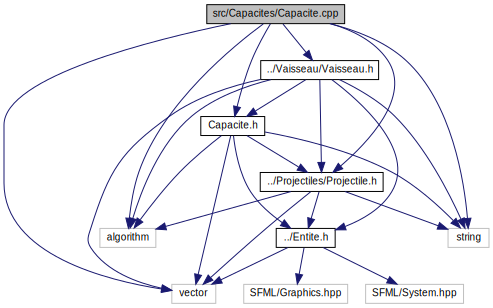
\includegraphics[width=350pt]{_capacite_8cpp__incl}
\end{center}
\end{figure}

\hypertarget{_capacite_8h}{}\section{Référence du fichier src/\+Capacite.h}
\label{_capacite_8h}\index{src/\+Capacite.\+h@{src/\+Capacite.\+h}}
\subsection*{Classes}
\begin{DoxyCompactItemize}
\item 
class \hyperlink{class_capacite}{Capacite}
\begin{DoxyCompactList}\small\item\em Classe virtuelle qui définit la structure générale d\textquotesingle{}une capacité \end{DoxyCompactList}\end{DoxyCompactItemize}

\hypertarget{_capacite_piou_piou_8cpp}{}\section{Référence du fichier src/\+Capacites/\+Capacite\+Piou\+Piou.cpp}
\label{_capacite_piou_piou_8cpp}\index{src/\+Capacites/\+Capacite\+Piou\+Piou.\+cpp@{src/\+Capacites/\+Capacite\+Piou\+Piou.\+cpp}}

\hypertarget{_capacite_piou_piou_8h}{}\section{Référence du fichier src/\+Capacites/\+Capacite\+Piou\+Piou.h}
\label{_capacite_piou_piou_8h}\index{src/\+Capacites/\+Capacite\+Piou\+Piou.\+h@{src/\+Capacites/\+Capacite\+Piou\+Piou.\+h}}

\hypertarget{_cap_dash_8cpp}{}\section{Référence du fichier src/\+Capacites/\+Cap\+Dash.cpp}
\label{_cap_dash_8cpp}\index{src/\+Capacites/\+Cap\+Dash.\+cpp@{src/\+Capacites/\+Cap\+Dash.\+cpp}}
{\ttfamily \#include \char`\"{}Cap\+Dash.\+h\char`\"{}}\newline
{\ttfamily \#include \char`\"{}../\+Interface/\+Input.\+h\char`\"{}}\newline
Graphe des dépendances par inclusion de Cap\+Dash.\+cpp\+:
% FIG 0

\hypertarget{_cap_dash_8h}{}\section{src/\+Capacites/\+Cap\+Dash.h File Reference}
\label{_cap_dash_8h}\index{src/\+Capacites/\+Cap\+Dash.\+h@{src/\+Capacites/\+Cap\+Dash.\+h}}
{\ttfamily \#include \char`\"{}Capacite.\+h\char`\"{}}\newline
{\ttfamily \#include \char`\"{}../\+Entite.\+h\char`\"{}}\newline
{\ttfamily \#include \char`\"{}../\+Projectiles/\+Proj\+Boing.\+h\char`\"{}}\newline
\subsection*{Classes}
\begin{DoxyCompactItemize}
\item 
class \mbox{\hyperlink{class_cap_dash}{Cap\+Dash}}
\begin{DoxyCompactList}\small\item\em Classe Capacité permettant de dash. \end{DoxyCompactList}\end{DoxyCompactItemize}

\hypertarget{_cap_piou_8cpp}{}\section{Référence du fichier src/\+Capacites/\+Cap\+Piou.cpp}
\label{_cap_piou_8cpp}\index{src/\+Capacites/\+Cap\+Piou.\+cpp@{src/\+Capacites/\+Cap\+Piou.\+cpp}}
{\ttfamily \#include \char`\"{}Cap\+Piou.\+h\char`\"{}}\newline
Graphe des dépendances par inclusion de Cap\+Piou.\+cpp\+:
\nopagebreak
\begin{figure}[H]
\begin{center}
\leavevmode
\includegraphics[width=350pt]{_cap_piou_8cpp__incl}
\end{center}
\end{figure}

\hypertarget{_cap_piou_8h}{}\section{Référence du fichier src/\+Capacites/\+Cap\+Piou.h}
\label{_cap_piou_8h}\index{src/\+Capacites/\+Cap\+Piou.\+h@{src/\+Capacites/\+Cap\+Piou.\+h}}
{\ttfamily \#include \char`\"{}Capacite.\+h\char`\"{}}\newline
{\ttfamily \#include \char`\"{}../\+Projectiles/\+Projectile.\+h\char`\"{}}\newline
{\ttfamily \#include \char`\"{}../\+Projectiles/\+Proj\+Piou.\+h\char`\"{}}\newline
Graphe des dépendances par inclusion de Cap\+Piou.\+h\+:
% FIG 0
Ce graphe montre quels fichiers incluent directement ou indirectement ce fichier \+:
% FIG 1
\subsection*{Classes}
\begin{DoxyCompactItemize}
\item 
class \hyperlink{class_cap_piou}{Cap\+Piou}
\begin{DoxyCompactList}\small\item\em Classe Capacité de base. \end{DoxyCompactList}\end{DoxyCompactItemize}

\hypertarget{_cap_test_8cpp}{}\section{Référence du fichier src/\+Capacites/\+Cap\+Test.cpp}
\label{_cap_test_8cpp}\index{src/\+Capacites/\+Cap\+Test.\+cpp@{src/\+Capacites/\+Cap\+Test.\+cpp}}
{\ttfamily \#include \char`\"{}Cap\+Test.\+h\char`\"{}}\newline
{\ttfamily \#include \char`\"{}Cap\+Dash.\+h\char`\"{}}\newline
Graphe des dépendances par inclusion de Cap\+Test.\+cpp\+:\nopagebreak
\begin{figure}[H]
\begin{center}
\leavevmode
\includegraphics[width=350pt]{_cap_test_8cpp__incl}
\end{center}
\end{figure}

\hypertarget{_cap_test_8h}{}\section{Référence du fichier src/\+Capacites/\+Cap\+Test.h}
\label{_cap_test_8h}\index{src/\+Capacites/\+Cap\+Test.\+h@{src/\+Capacites/\+Cap\+Test.\+h}}
{\ttfamily \#include \char`\"{}Capacite.\+h\char`\"{}}\newline
{\ttfamily \#include \char`\"{}../\+Projectiles/\+Projectile.\+h\char`\"{}}\newline
{\ttfamily \#include \char`\"{}../\+Projectiles/\+Proj\+Test.\+h\char`\"{}}\newline
Graphe des dépendances par inclusion de Cap\+Test.\+h\+:\nopagebreak
\begin{figure}[H]
\begin{center}
\leavevmode
\includegraphics[width=350pt]{_cap_test_8h__incl}
\end{center}
\end{figure}
Ce graphe montre quels fichiers incluent directement ou indirectement ce fichier \+:\nopagebreak
\begin{figure}[H]
\begin{center}
\leavevmode
\includegraphics[width=350pt]{_cap_test_8h__dep__incl}
\end{center}
\end{figure}
\subsection*{Classes}
\begin{DoxyCompactItemize}
\item 
class \hyperlink{class_cap_test}{Cap\+Test}
\end{DoxyCompactItemize}

\hypertarget{_collision_8cpp}{}\section{Référence du fichier src/\+Utilitaires/\+Collision.cpp}
\label{_collision_8cpp}\index{src/\+Utilitaires/\+Collision.\+cpp@{src/\+Utilitaires/\+Collision.\+cpp}}
{\ttfamily \#include \char`\"{}Collision.\+h\char`\"{}}\newline
{\ttfamily \#include $<$cmath$>$}\newline
Graphe des dépendances par inclusion de Collision.\+cpp\+:\nopagebreak
\begin{figure}[H]
\begin{center}
\leavevmode
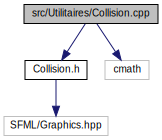
\includegraphics[width=234pt]{_collision_8cpp__incl}
\end{center}
\end{figure}
\subsection*{Fonctions}
\begin{DoxyCompactItemize}
\item 
sf\+::\+Vector2f \hyperlink{_collision_8cpp_a19be16a0d78cc53699ec1f6cc1247f0a}{centre\+\_\+transforme} (const sf\+::\+Circle\+Shape \&c)
\item 
sf\+::\+Vector2f \hyperlink{_collision_8cpp_aaf8f0e4613fb5a09397a7825b1ff4909}{point\+\_\+transforme} (const sf\+::\+Shape \&s, size\+\_\+t index)
\item 
bool \hyperlink{_collision_8cpp_a55cd5d990d317edd263c1d3bcd0b5a05}{is\+\_\+point\+\_\+in} (const sf\+::\+Vector2f \&C, const sf\+::\+Shape \&s)
\item 
bool \hyperlink{_collision_8cpp_a9037d2ebead3fc780ff50019012ac010}{collision} (const sf\+::\+Shape \&s1, const sf\+::\+Shape \&s2)
\item 
bool \hyperlink{_collision_8cpp_a4a4d2e91bbfd88f8aaaeb1572140a024}{collision\+\_\+impl} (const sf\+::\+Circle\+Shape \&c1, const sf\+::\+Circle\+Shape \&c2)
\item 
bool \hyperlink{_collision_8cpp_a598969c4bf7355123d972d3cf69eafd5}{collision\+\_\+impl} (const sf\+::\+Circle\+Shape \&c, const sf\+::\+Shape \&co)
\item 
bool \hyperlink{_collision_8cpp_adcae147b4b5b0ca770cfbc5b1c65873d}{collision\+\_\+impl} (const sf\+::\+Shape \&co, const sf\+::\+Circle\+Shape \&c)
\item 
bool \hyperlink{_collision_8cpp_ad5b149f81d5c820b0f81e5ca66385dee}{collision\+\_\+impl} (const sf\+::\+Shape \&s1, const sf\+::\+Shape \&s2)
\end{DoxyCompactItemize}
\subsection*{Variables}
\begin{DoxyCompactItemize}
\item 
const double \hyperlink{_collision_8cpp_a952eac791b596a61bba0a133a3bb439f}{PI} = acos(-\/1)
\end{DoxyCompactItemize}


\subsection{Documentation des fonctions}
\mbox{\Hypertarget{_collision_8cpp_a19be16a0d78cc53699ec1f6cc1247f0a}\label{_collision_8cpp_a19be16a0d78cc53699ec1f6cc1247f0a}} 
\index{Collision.\+cpp@{Collision.\+cpp}!centre\+\_\+transforme@{centre\+\_\+transforme}}
\index{centre\+\_\+transforme@{centre\+\_\+transforme}!Collision.\+cpp@{Collision.\+cpp}}
\subsubsection{\texorpdfstring{centre\+\_\+transforme()}{centre\_transforme()}}
{\footnotesize\ttfamily sf\+::\+Vector2f centre\+\_\+transforme (\begin{DoxyParamCaption}\item[{const sf\+::\+Circle\+Shape \&}]{c }\end{DoxyParamCaption})}

\mbox{\Hypertarget{_collision_8cpp_a9037d2ebead3fc780ff50019012ac010}\label{_collision_8cpp_a9037d2ebead3fc780ff50019012ac010}} 
\index{Collision.\+cpp@{Collision.\+cpp}!collision@{collision}}
\index{collision@{collision}!Collision.\+cpp@{Collision.\+cpp}}
\subsubsection{\texorpdfstring{collision()}{collision()}}
{\footnotesize\ttfamily bool collision (\begin{DoxyParamCaption}\item[{const sf\+::\+Shape \&}]{s1,  }\item[{const sf\+::\+Shape \&}]{s2 }\end{DoxyParamCaption})}

\mbox{\Hypertarget{_collision_8cpp_a4a4d2e91bbfd88f8aaaeb1572140a024}\label{_collision_8cpp_a4a4d2e91bbfd88f8aaaeb1572140a024}} 
\index{Collision.\+cpp@{Collision.\+cpp}!collision\+\_\+impl@{collision\+\_\+impl}}
\index{collision\+\_\+impl@{collision\+\_\+impl}!Collision.\+cpp@{Collision.\+cpp}}
\subsubsection{\texorpdfstring{collision\+\_\+impl()}{collision\_impl()}\hspace{0.1cm}{\footnotesize\ttfamily [1/4]}}
{\footnotesize\ttfamily bool collision\+\_\+impl (\begin{DoxyParamCaption}\item[{const sf\+::\+Circle\+Shape \&}]{c1,  }\item[{const sf\+::\+Circle\+Shape \&}]{c2 }\end{DoxyParamCaption})}

\mbox{\Hypertarget{_collision_8cpp_a598969c4bf7355123d972d3cf69eafd5}\label{_collision_8cpp_a598969c4bf7355123d972d3cf69eafd5}} 
\index{Collision.\+cpp@{Collision.\+cpp}!collision\+\_\+impl@{collision\+\_\+impl}}
\index{collision\+\_\+impl@{collision\+\_\+impl}!Collision.\+cpp@{Collision.\+cpp}}
\subsubsection{\texorpdfstring{collision\+\_\+impl()}{collision\_impl()}\hspace{0.1cm}{\footnotesize\ttfamily [2/4]}}
{\footnotesize\ttfamily bool collision\+\_\+impl (\begin{DoxyParamCaption}\item[{const sf\+::\+Circle\+Shape \&}]{c,  }\item[{const sf\+::\+Shape \&}]{co }\end{DoxyParamCaption})}

\mbox{\Hypertarget{_collision_8cpp_adcae147b4b5b0ca770cfbc5b1c65873d}\label{_collision_8cpp_adcae147b4b5b0ca770cfbc5b1c65873d}} 
\index{Collision.\+cpp@{Collision.\+cpp}!collision\+\_\+impl@{collision\+\_\+impl}}
\index{collision\+\_\+impl@{collision\+\_\+impl}!Collision.\+cpp@{Collision.\+cpp}}
\subsubsection{\texorpdfstring{collision\+\_\+impl()}{collision\_impl()}\hspace{0.1cm}{\footnotesize\ttfamily [3/4]}}
{\footnotesize\ttfamily bool collision\+\_\+impl (\begin{DoxyParamCaption}\item[{const sf\+::\+Shape \&}]{co,  }\item[{const sf\+::\+Circle\+Shape \&}]{c }\end{DoxyParamCaption})}

\mbox{\Hypertarget{_collision_8cpp_ad5b149f81d5c820b0f81e5ca66385dee}\label{_collision_8cpp_ad5b149f81d5c820b0f81e5ca66385dee}} 
\index{Collision.\+cpp@{Collision.\+cpp}!collision\+\_\+impl@{collision\+\_\+impl}}
\index{collision\+\_\+impl@{collision\+\_\+impl}!Collision.\+cpp@{Collision.\+cpp}}
\subsubsection{\texorpdfstring{collision\+\_\+impl()}{collision\_impl()}\hspace{0.1cm}{\footnotesize\ttfamily [4/4]}}
{\footnotesize\ttfamily bool collision\+\_\+impl (\begin{DoxyParamCaption}\item[{const sf\+::\+Shape \&}]{s1,  }\item[{const sf\+::\+Shape \&}]{s2 }\end{DoxyParamCaption})}

\mbox{\Hypertarget{_collision_8cpp_a55cd5d990d317edd263c1d3bcd0b5a05}\label{_collision_8cpp_a55cd5d990d317edd263c1d3bcd0b5a05}} 
\index{Collision.\+cpp@{Collision.\+cpp}!is\+\_\+point\+\_\+in@{is\+\_\+point\+\_\+in}}
\index{is\+\_\+point\+\_\+in@{is\+\_\+point\+\_\+in}!Collision.\+cpp@{Collision.\+cpp}}
\subsubsection{\texorpdfstring{is\+\_\+point\+\_\+in()}{is\_point\_in()}}
{\footnotesize\ttfamily bool is\+\_\+point\+\_\+in (\begin{DoxyParamCaption}\item[{const sf\+::\+Vector2f \&}]{C,  }\item[{const sf\+::\+Shape \&}]{s }\end{DoxyParamCaption})}

\mbox{\Hypertarget{_collision_8cpp_aaf8f0e4613fb5a09397a7825b1ff4909}\label{_collision_8cpp_aaf8f0e4613fb5a09397a7825b1ff4909}} 
\index{Collision.\+cpp@{Collision.\+cpp}!point\+\_\+transforme@{point\+\_\+transforme}}
\index{point\+\_\+transforme@{point\+\_\+transforme}!Collision.\+cpp@{Collision.\+cpp}}
\subsubsection{\texorpdfstring{point\+\_\+transforme()}{point\_transforme()}}
{\footnotesize\ttfamily sf\+::\+Vector2f point\+\_\+transforme (\begin{DoxyParamCaption}\item[{const sf\+::\+Shape \&}]{s,  }\item[{size\+\_\+t}]{index }\end{DoxyParamCaption})}



\subsection{Documentation des variables}
\mbox{\Hypertarget{_collision_8cpp_a952eac791b596a61bba0a133a3bb439f}\label{_collision_8cpp_a952eac791b596a61bba0a133a3bb439f}} 
\index{Collision.\+cpp@{Collision.\+cpp}!PI@{PI}}
\index{PI@{PI}!Collision.\+cpp@{Collision.\+cpp}}
\subsubsection{\texorpdfstring{PI}{PI}}
{\footnotesize\ttfamily const double PI = acos(-\/1)}


\hypertarget{_collision_8h}{}\section{Référence du fichier src/\+Collision.h}
\label{_collision_8h}\index{src/\+Collision.\+h@{src/\+Collision.\+h}}
{\ttfamily \#include $<$S\+F\+M\+L/\+Graphics.\+hpp$>$}\newline
Graphe des dépendances par inclusion de Collision.\+h\+:\nopagebreak
\begin{figure}[H]
\begin{center}
\leavevmode
\includegraphics[width=184pt]{_collision_8h__incl}
\end{center}
\end{figure}
Ce graphe montre quels fichiers incluent directement ou indirectement ce fichier \+:\nopagebreak
\begin{figure}[H]
\begin{center}
\leavevmode
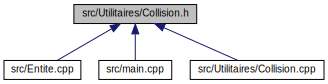
\includegraphics[width=350pt]{_collision_8h__dep__incl}
\end{center}
\end{figure}
\subsection*{Fonctions}
\begin{DoxyCompactItemize}
\item 
bool \hyperlink{_collision_8h_a9037d2ebead3fc780ff50019012ac010}{collision} (const sf\+::\+Shape \&s1, const sf\+::\+Shape \&s2)
\item 
bool \hyperlink{_collision_8h_ad5b149f81d5c820b0f81e5ca66385dee}{collision\+\_\+impl} (const sf\+::\+Shape \&s1, const sf\+::\+Shape \&s2)
\item 
bool \hyperlink{_collision_8h_a4a4d2e91bbfd88f8aaaeb1572140a024}{collision\+\_\+impl} (const sf\+::\+Circle\+Shape \&c1, const sf\+::\+Circle\+Shape \&c2)
\item 
bool \hyperlink{_collision_8h_a598969c4bf7355123d972d3cf69eafd5}{collision\+\_\+impl} (const sf\+::\+Circle\+Shape \&c, const sf\+::\+Shape \&co)
\item 
bool \hyperlink{_collision_8h_adcae147b4b5b0ca770cfbc5b1c65873d}{collision\+\_\+impl} (const sf\+::\+Shape \&co, const sf\+::\+Circle\+Shape \&c)
\end{DoxyCompactItemize}


\subsection{Documentation des fonctions}
\mbox{\Hypertarget{_collision_8h_a9037d2ebead3fc780ff50019012ac010}\label{_collision_8h_a9037d2ebead3fc780ff50019012ac010}} 
\index{Collision.\+h@{Collision.\+h}!collision@{collision}}
\index{collision@{collision}!Collision.\+h@{Collision.\+h}}
\subsubsection{\texorpdfstring{collision()}{collision()}}
{\footnotesize\ttfamily bool collision (\begin{DoxyParamCaption}\item[{const sf\+::\+Shape \&}]{s1,  }\item[{const sf\+::\+Shape \&}]{s2 }\end{DoxyParamCaption})}

\mbox{\Hypertarget{_collision_8h_ad5b149f81d5c820b0f81e5ca66385dee}\label{_collision_8h_ad5b149f81d5c820b0f81e5ca66385dee}} 
\index{Collision.\+h@{Collision.\+h}!collision\+\_\+impl@{collision\+\_\+impl}}
\index{collision\+\_\+impl@{collision\+\_\+impl}!Collision.\+h@{Collision.\+h}}
\subsubsection{\texorpdfstring{collision\+\_\+impl()}{collision\_impl()}\hspace{0.1cm}{\footnotesize\ttfamily [1/4]}}
{\footnotesize\ttfamily bool collision\+\_\+impl (\begin{DoxyParamCaption}\item[{const sf\+::\+Shape \&}]{s1,  }\item[{const sf\+::\+Shape \&}]{s2 }\end{DoxyParamCaption})}

\mbox{\Hypertarget{_collision_8h_a4a4d2e91bbfd88f8aaaeb1572140a024}\label{_collision_8h_a4a4d2e91bbfd88f8aaaeb1572140a024}} 
\index{Collision.\+h@{Collision.\+h}!collision\+\_\+impl@{collision\+\_\+impl}}
\index{collision\+\_\+impl@{collision\+\_\+impl}!Collision.\+h@{Collision.\+h}}
\subsubsection{\texorpdfstring{collision\+\_\+impl()}{collision\_impl()}\hspace{0.1cm}{\footnotesize\ttfamily [2/4]}}
{\footnotesize\ttfamily bool collision\+\_\+impl (\begin{DoxyParamCaption}\item[{const sf\+::\+Circle\+Shape \&}]{c1,  }\item[{const sf\+::\+Circle\+Shape \&}]{c2 }\end{DoxyParamCaption})}

\mbox{\Hypertarget{_collision_8h_a598969c4bf7355123d972d3cf69eafd5}\label{_collision_8h_a598969c4bf7355123d972d3cf69eafd5}} 
\index{Collision.\+h@{Collision.\+h}!collision\+\_\+impl@{collision\+\_\+impl}}
\index{collision\+\_\+impl@{collision\+\_\+impl}!Collision.\+h@{Collision.\+h}}
\subsubsection{\texorpdfstring{collision\+\_\+impl()}{collision\_impl()}\hspace{0.1cm}{\footnotesize\ttfamily [3/4]}}
{\footnotesize\ttfamily bool collision\+\_\+impl (\begin{DoxyParamCaption}\item[{const sf\+::\+Circle\+Shape \&}]{c,  }\item[{const sf\+::\+Shape \&}]{co }\end{DoxyParamCaption})}

\mbox{\Hypertarget{_collision_8h_adcae147b4b5b0ca770cfbc5b1c65873d}\label{_collision_8h_adcae147b4b5b0ca770cfbc5b1c65873d}} 
\index{Collision.\+h@{Collision.\+h}!collision\+\_\+impl@{collision\+\_\+impl}}
\index{collision\+\_\+impl@{collision\+\_\+impl}!Collision.\+h@{Collision.\+h}}
\subsubsection{\texorpdfstring{collision\+\_\+impl()}{collision\_impl()}\hspace{0.1cm}{\footnotesize\ttfamily [4/4]}}
{\footnotesize\ttfamily bool collision\+\_\+impl (\begin{DoxyParamCaption}\item[{const sf\+::\+Shape \&}]{co,  }\item[{const sf\+::\+Circle\+Shape \&}]{c }\end{DoxyParamCaption})}


\hypertarget{constantes_8h}{}\section{src/constantes.h File Reference}
\label{constantes_8h}\index{src/constantes.\+h@{src/constantes.\+h}}
{\ttfamily \#include $<$cstddef$>$}\newline
\subsection*{Macros}
\begin{DoxyCompactItemize}
\item 
\#define \mbox{\hyperlink{constantes_8h_aa55807c5b694c7cefe344e8b78e5aadb}{chemin\+\_\+rc}}~\char`\"{}../../rc/\char`\"{}
\item 
\#define \mbox{\hyperlink{constantes_8h_a598a3330b3c21701223ee0ca14316eca}{PI}}~acos(-\/1.\+0)
\item 
\#define \mbox{\hyperlink{constantes_8h_a1c6d5de492ac61ad29aec7aa9a436bbf}{V\+E\+R\+S\+I\+ON}}~\char`\"{}Debug.\char`\"{}
\item 
\#define \mbox{\hyperlink{constantes_8h_ad9816adb4ece0656cd3d58f627b107db}{B\+R\+A\+N\+C\+HE}}~\char`\"{}Nettoyage de printemps\char`\"{}
\end{DoxyCompactItemize}
\subsection*{Enumerations}
\begin{DoxyCompactItemize}
\item 
enum \mbox{\hyperlink{constantes_8h_a250372292659bed7ae290d8621f88ccf}{Actions}} \{ \newline
\mbox{\hyperlink{constantes_8h_a250372292659bed7ae290d8621f88ccfa56b36d0d0bb01b339cf1041adc08e262}{P\+A\+U\+SE}}, 
\mbox{\hyperlink{constantes_8h_a250372292659bed7ae290d8621f88ccfa44466ad40cb0a09371d2b828b36c48e7}{T\+I\+R1}}, 
\mbox{\hyperlink{constantes_8h_a250372292659bed7ae290d8621f88ccfac9439845b5972a9dc101085343ac065c}{T\+I\+R2}}, 
\mbox{\hyperlink{constantes_8h_a250372292659bed7ae290d8621f88ccfa157fc740ff7ff2c0247ac5961f66009c}{C\+O\+M\+P1}}, 
\newline
\mbox{\hyperlink{constantes_8h_a250372292659bed7ae290d8621f88ccfa56bb8c406fa7684dc34ffe1a6d389565}{C\+O\+M\+P2}}, 
\mbox{\hyperlink{constantes_8h_a250372292659bed7ae290d8621f88ccfaccc8850f02d2db3d2e39bec5295edc46}{C\+O\+M\+P3}}, 
\mbox{\hyperlink{constantes_8h_a250372292659bed7ae290d8621f88ccfa26cfa63737372a3312d10aebb767d603}{U\+L\+TI}}
 \}
\item 
enum \mbox{\hyperlink{constantes_8h_a08fa5554288d5031a8f3bb83cc04ee83}{Equipe}} \{ \mbox{\hyperlink{constantes_8h_a08fa5554288d5031a8f3bb83cc04ee83ad4d15427af4b5b0f54dbed84f89cade7}{J\+O\+U\+E\+UR}}, 
\mbox{\hyperlink{constantes_8h_a08fa5554288d5031a8f3bb83cc04ee83a6c21d8eea108820375064b6acafce3f9}{E\+N\+N\+E\+MI}}, 
\mbox{\hyperlink{constantes_8h_a08fa5554288d5031a8f3bb83cc04ee83a31ad00d2974deb1103ea000de3bff57d}{N\+E\+U\+T\+RE}}, 
\mbox{\hyperlink{constantes_8h_a08fa5554288d5031a8f3bb83cc04ee83a720a6a0fa0be9398650409a7befa7293}{A\+L\+L\+IE}}
 \}
\item 
enum \mbox{\hyperlink{constantes_8h_a33e4f15dde10f34860a6b35be343ae56}{ecran\+\_\+t}} \{ \mbox{\hyperlink{constantes_8h_a33e4f15dde10f34860a6b35be343ae56ad4686f4f969d0e851d9170c09a89a837}{V\+I\+DE}} = -\/1, 
\mbox{\hyperlink{constantes_8h_a33e4f15dde10f34860a6b35be343ae56a96251739b593a8e10380d58a30e93fd8}{A\+C\+C\+U\+E\+IL}} = 0, 
\mbox{\hyperlink{constantes_8h_a33e4f15dde10f34860a6b35be343ae56ad84154820fb7cc5480aa99b8e888ef2e}{M\+E\+N\+U\+\_\+\+P\+R\+I\+N\+C\+I\+P\+AL}}, 
\mbox{\hyperlink{constantes_8h_a33e4f15dde10f34860a6b35be343ae56adb639f85bf0a305a48b5874ea027a831}{P\+A\+R\+T\+IE}}
 \}
\end{DoxyCompactItemize}
\subsection*{Variables}
\begin{DoxyCompactItemize}
\item 
constexpr float \mbox{\hyperlink{constantes_8h_a8958557e953d458537dedcf460f477c1}{E\+C\+R\+A\+N\+\_\+L}} = 1024
\item 
constexpr float \mbox{\hyperlink{constantes_8h_a899c06d4fdb39f4fa51fc7158e2be2d1}{E\+C\+R\+A\+N\+\_\+H}} = 768
\begin{DoxyCompactList}\small\item\em Largueur de la fenetre. \end{DoxyCompactList}\item 
constexpr float \mbox{\hyperlink{constantes_8h_ac48605b788819fe8dcad2622d7f1f00c}{O\+V\+E\+R\+L\+A\+Y\+\_\+\+B\+A\+R\+R\+E\+\_\+L}} = 500
\begin{DoxyCompactList}\small\item\em Hauteur de la fenetre. \end{DoxyCompactList}\item 
constexpr float \mbox{\hyperlink{constantes_8h_aec53a7a575e951f65fca395d860ff1c6}{O\+V\+E\+R\+L\+A\+Y\+\_\+\+B\+A\+R\+R\+E\+\_\+H}} = 16
\begin{DoxyCompactList}\small\item\em Largueur des barres de l\textquotesingle{}overlay. \end{DoxyCompactList}\item 
constexpr size\+\_\+t \mbox{\hyperlink{constantes_8h_abd929aee9ec2e5d880b87ac867ad49e1}{N\+B\+\_\+\+A\+C\+T\+I\+ON}} = 7
\begin{DoxyCompactList}\small\item\em Hauteur des barres de l\textquotesingle{}overlay. \end{DoxyCompactList}\item 
constexpr size\+\_\+t \mbox{\hyperlink{constantes_8h_ad4a41a3da7bd10b3350047db17a78ee6}{T\+E\+M\+P\+S\+\_\+\+I\+N\+V\+I\+N\+C\+I\+B\+I\+L\+I\+TE}} = 2000
\begin{DoxyCompactList}\small\item\em Nombre d\textquotesingle{}actions. \end{DoxyCompactList}\item 
constexpr bool \mbox{\hyperlink{constantes_8h_a7507bfee1d3f050ad869013d74424e9e}{D\+E\+B\+UG}} = true
\begin{DoxyCompactList}\small\item\em Nombres de millisecondes d\textquotesingle{}invincibilité par défaut. \end{DoxyCompactList}\end{DoxyCompactItemize}


\subsection{Macro Definition Documentation}
\mbox{\Hypertarget{constantes_8h_ad9816adb4ece0656cd3d58f627b107db}\label{constantes_8h_ad9816adb4ece0656cd3d58f627b107db}} 
\index{constantes.\+h@{constantes.\+h}!B\+R\+A\+N\+C\+HE@{B\+R\+A\+N\+C\+HE}}
\index{B\+R\+A\+N\+C\+HE@{B\+R\+A\+N\+C\+HE}!constantes.\+h@{constantes.\+h}}
\subsubsection{\texorpdfstring{B\+R\+A\+N\+C\+HE}{BRANCHE}}
{\footnotesize\ttfamily \#define B\+R\+A\+N\+C\+HE~\char`\"{}Nettoyage de printemps\char`\"{}}

\mbox{\Hypertarget{constantes_8h_aa55807c5b694c7cefe344e8b78e5aadb}\label{constantes_8h_aa55807c5b694c7cefe344e8b78e5aadb}} 
\index{constantes.\+h@{constantes.\+h}!chemin\+\_\+rc@{chemin\+\_\+rc}}
\index{chemin\+\_\+rc@{chemin\+\_\+rc}!constantes.\+h@{constantes.\+h}}
\subsubsection{\texorpdfstring{chemin\+\_\+rc}{chemin\_rc}}
{\footnotesize\ttfamily \#define chemin\+\_\+rc~\char`\"{}../../rc/\char`\"{}}

\mbox{\Hypertarget{constantes_8h_a598a3330b3c21701223ee0ca14316eca}\label{constantes_8h_a598a3330b3c21701223ee0ca14316eca}} 
\index{constantes.\+h@{constantes.\+h}!PI@{PI}}
\index{PI@{PI}!constantes.\+h@{constantes.\+h}}
\subsubsection{\texorpdfstring{PI}{PI}}
{\footnotesize\ttfamily \#define PI~acos(-\/1.\+0)}

\mbox{\Hypertarget{constantes_8h_a1c6d5de492ac61ad29aec7aa9a436bbf}\label{constantes_8h_a1c6d5de492ac61ad29aec7aa9a436bbf}} 
\index{constantes.\+h@{constantes.\+h}!V\+E\+R\+S\+I\+ON@{V\+E\+R\+S\+I\+ON}}
\index{V\+E\+R\+S\+I\+ON@{V\+E\+R\+S\+I\+ON}!constantes.\+h@{constantes.\+h}}
\subsubsection{\texorpdfstring{V\+E\+R\+S\+I\+ON}{VERSION}}
{\footnotesize\ttfamily \#define V\+E\+R\+S\+I\+ON~\char`\"{}Debug.\char`\"{}}



\subsection{Enumeration Type Documentation}
\mbox{\Hypertarget{constantes_8h_a250372292659bed7ae290d8621f88ccf}\label{constantes_8h_a250372292659bed7ae290d8621f88ccf}} 
\index{constantes.\+h@{constantes.\+h}!Actions@{Actions}}
\index{Actions@{Actions}!constantes.\+h@{constantes.\+h}}
\subsubsection{\texorpdfstring{Actions}{Actions}}
{\footnotesize\ttfamily enum \mbox{\hyperlink{constantes_8h_a250372292659bed7ae290d8621f88ccf}{Actions}}}

\begin{DoxyEnumFields}{Enumerator}
\raisebox{\heightof{T}}[0pt][0pt]{\index{P\+A\+U\+SE@{P\+A\+U\+SE}!constantes.\+h@{constantes.\+h}}\index{constantes.\+h@{constantes.\+h}!P\+A\+U\+SE@{P\+A\+U\+SE}}}\mbox{\Hypertarget{constantes_8h_a250372292659bed7ae290d8621f88ccfa56b36d0d0bb01b339cf1041adc08e262}\label{constantes_8h_a250372292659bed7ae290d8621f88ccfa56b36d0d0bb01b339cf1041adc08e262}} 
P\+A\+U\+SE&\\
\hline

\raisebox{\heightof{T}}[0pt][0pt]{\index{T\+I\+R1@{T\+I\+R1}!constantes.\+h@{constantes.\+h}}\index{constantes.\+h@{constantes.\+h}!T\+I\+R1@{T\+I\+R1}}}\mbox{\Hypertarget{constantes_8h_a250372292659bed7ae290d8621f88ccfa44466ad40cb0a09371d2b828b36c48e7}\label{constantes_8h_a250372292659bed7ae290d8621f88ccfa44466ad40cb0a09371d2b828b36c48e7}} 
T\+I\+R1&\\
\hline

\raisebox{\heightof{T}}[0pt][0pt]{\index{T\+I\+R2@{T\+I\+R2}!constantes.\+h@{constantes.\+h}}\index{constantes.\+h@{constantes.\+h}!T\+I\+R2@{T\+I\+R2}}}\mbox{\Hypertarget{constantes_8h_a250372292659bed7ae290d8621f88ccfac9439845b5972a9dc101085343ac065c}\label{constantes_8h_a250372292659bed7ae290d8621f88ccfac9439845b5972a9dc101085343ac065c}} 
T\+I\+R2&\\
\hline

\raisebox{\heightof{T}}[0pt][0pt]{\index{C\+O\+M\+P1@{C\+O\+M\+P1}!constantes.\+h@{constantes.\+h}}\index{constantes.\+h@{constantes.\+h}!C\+O\+M\+P1@{C\+O\+M\+P1}}}\mbox{\Hypertarget{constantes_8h_a250372292659bed7ae290d8621f88ccfa157fc740ff7ff2c0247ac5961f66009c}\label{constantes_8h_a250372292659bed7ae290d8621f88ccfa157fc740ff7ff2c0247ac5961f66009c}} 
C\+O\+M\+P1&\\
\hline

\raisebox{\heightof{T}}[0pt][0pt]{\index{C\+O\+M\+P2@{C\+O\+M\+P2}!constantes.\+h@{constantes.\+h}}\index{constantes.\+h@{constantes.\+h}!C\+O\+M\+P2@{C\+O\+M\+P2}}}\mbox{\Hypertarget{constantes_8h_a250372292659bed7ae290d8621f88ccfa56bb8c406fa7684dc34ffe1a6d389565}\label{constantes_8h_a250372292659bed7ae290d8621f88ccfa56bb8c406fa7684dc34ffe1a6d389565}} 
C\+O\+M\+P2&\\
\hline

\raisebox{\heightof{T}}[0pt][0pt]{\index{C\+O\+M\+P3@{C\+O\+M\+P3}!constantes.\+h@{constantes.\+h}}\index{constantes.\+h@{constantes.\+h}!C\+O\+M\+P3@{C\+O\+M\+P3}}}\mbox{\Hypertarget{constantes_8h_a250372292659bed7ae290d8621f88ccfaccc8850f02d2db3d2e39bec5295edc46}\label{constantes_8h_a250372292659bed7ae290d8621f88ccfaccc8850f02d2db3d2e39bec5295edc46}} 
C\+O\+M\+P3&\\
\hline

\raisebox{\heightof{T}}[0pt][0pt]{\index{U\+L\+TI@{U\+L\+TI}!constantes.\+h@{constantes.\+h}}\index{constantes.\+h@{constantes.\+h}!U\+L\+TI@{U\+L\+TI}}}\mbox{\Hypertarget{constantes_8h_a250372292659bed7ae290d8621f88ccfa26cfa63737372a3312d10aebb767d603}\label{constantes_8h_a250372292659bed7ae290d8621f88ccfa26cfa63737372a3312d10aebb767d603}} 
U\+L\+TI&\\
\hline

\end{DoxyEnumFields}
\mbox{\Hypertarget{constantes_8h_a33e4f15dde10f34860a6b35be343ae56}\label{constantes_8h_a33e4f15dde10f34860a6b35be343ae56}} 
\index{constantes.\+h@{constantes.\+h}!ecran\+\_\+t@{ecran\+\_\+t}}
\index{ecran\+\_\+t@{ecran\+\_\+t}!constantes.\+h@{constantes.\+h}}
\subsubsection{\texorpdfstring{ecran\+\_\+t}{ecran\_t}}
{\footnotesize\ttfamily enum \mbox{\hyperlink{constantes_8h_a33e4f15dde10f34860a6b35be343ae56}{ecran\+\_\+t}}}

\begin{DoxyEnumFields}{Enumerator}
\raisebox{\heightof{T}}[0pt][0pt]{\index{V\+I\+DE@{V\+I\+DE}!constantes.\+h@{constantes.\+h}}\index{constantes.\+h@{constantes.\+h}!V\+I\+DE@{V\+I\+DE}}}\mbox{\Hypertarget{constantes_8h_a33e4f15dde10f34860a6b35be343ae56ad4686f4f969d0e851d9170c09a89a837}\label{constantes_8h_a33e4f15dde10f34860a6b35be343ae56ad4686f4f969d0e851d9170c09a89a837}} 
V\+I\+DE&\\
\hline

\raisebox{\heightof{T}}[0pt][0pt]{\index{A\+C\+C\+U\+E\+IL@{A\+C\+C\+U\+E\+IL}!constantes.\+h@{constantes.\+h}}\index{constantes.\+h@{constantes.\+h}!A\+C\+C\+U\+E\+IL@{A\+C\+C\+U\+E\+IL}}}\mbox{\Hypertarget{constantes_8h_a33e4f15dde10f34860a6b35be343ae56a96251739b593a8e10380d58a30e93fd8}\label{constantes_8h_a33e4f15dde10f34860a6b35be343ae56a96251739b593a8e10380d58a30e93fd8}} 
A\+C\+C\+U\+E\+IL&\\
\hline

\raisebox{\heightof{T}}[0pt][0pt]{\index{M\+E\+N\+U\+\_\+\+P\+R\+I\+N\+C\+I\+P\+AL@{M\+E\+N\+U\+\_\+\+P\+R\+I\+N\+C\+I\+P\+AL}!constantes.\+h@{constantes.\+h}}\index{constantes.\+h@{constantes.\+h}!M\+E\+N\+U\+\_\+\+P\+R\+I\+N\+C\+I\+P\+AL@{M\+E\+N\+U\+\_\+\+P\+R\+I\+N\+C\+I\+P\+AL}}}\mbox{\Hypertarget{constantes_8h_a33e4f15dde10f34860a6b35be343ae56ad84154820fb7cc5480aa99b8e888ef2e}\label{constantes_8h_a33e4f15dde10f34860a6b35be343ae56ad84154820fb7cc5480aa99b8e888ef2e}} 
M\+E\+N\+U\+\_\+\+P\+R\+I\+N\+C\+I\+P\+AL&\\
\hline

\raisebox{\heightof{T}}[0pt][0pt]{\index{P\+A\+R\+T\+IE@{P\+A\+R\+T\+IE}!constantes.\+h@{constantes.\+h}}\index{constantes.\+h@{constantes.\+h}!P\+A\+R\+T\+IE@{P\+A\+R\+T\+IE}}}\mbox{\Hypertarget{constantes_8h_a33e4f15dde10f34860a6b35be343ae56adb639f85bf0a305a48b5874ea027a831}\label{constantes_8h_a33e4f15dde10f34860a6b35be343ae56adb639f85bf0a305a48b5874ea027a831}} 
P\+A\+R\+T\+IE&\\
\hline

\end{DoxyEnumFields}
\mbox{\Hypertarget{constantes_8h_a08fa5554288d5031a8f3bb83cc04ee83}\label{constantes_8h_a08fa5554288d5031a8f3bb83cc04ee83}} 
\index{constantes.\+h@{constantes.\+h}!Equipe@{Equipe}}
\index{Equipe@{Equipe}!constantes.\+h@{constantes.\+h}}
\subsubsection{\texorpdfstring{Equipe}{Equipe}}
{\footnotesize\ttfamily enum \mbox{\hyperlink{constantes_8h_a08fa5554288d5031a8f3bb83cc04ee83}{Equipe}}}

\begin{DoxyEnumFields}{Enumerator}
\raisebox{\heightof{T}}[0pt][0pt]{\index{J\+O\+U\+E\+UR@{J\+O\+U\+E\+UR}!constantes.\+h@{constantes.\+h}}\index{constantes.\+h@{constantes.\+h}!J\+O\+U\+E\+UR@{J\+O\+U\+E\+UR}}}\mbox{\Hypertarget{constantes_8h_a08fa5554288d5031a8f3bb83cc04ee83ad4d15427af4b5b0f54dbed84f89cade7}\label{constantes_8h_a08fa5554288d5031a8f3bb83cc04ee83ad4d15427af4b5b0f54dbed84f89cade7}} 
J\+O\+U\+E\+UR&\\
\hline

\raisebox{\heightof{T}}[0pt][0pt]{\index{E\+N\+N\+E\+MI@{E\+N\+N\+E\+MI}!constantes.\+h@{constantes.\+h}}\index{constantes.\+h@{constantes.\+h}!E\+N\+N\+E\+MI@{E\+N\+N\+E\+MI}}}\mbox{\Hypertarget{constantes_8h_a08fa5554288d5031a8f3bb83cc04ee83a6c21d8eea108820375064b6acafce3f9}\label{constantes_8h_a08fa5554288d5031a8f3bb83cc04ee83a6c21d8eea108820375064b6acafce3f9}} 
E\+N\+N\+E\+MI&\\
\hline

\raisebox{\heightof{T}}[0pt][0pt]{\index{N\+E\+U\+T\+RE@{N\+E\+U\+T\+RE}!constantes.\+h@{constantes.\+h}}\index{constantes.\+h@{constantes.\+h}!N\+E\+U\+T\+RE@{N\+E\+U\+T\+RE}}}\mbox{\Hypertarget{constantes_8h_a08fa5554288d5031a8f3bb83cc04ee83a31ad00d2974deb1103ea000de3bff57d}\label{constantes_8h_a08fa5554288d5031a8f3bb83cc04ee83a31ad00d2974deb1103ea000de3bff57d}} 
N\+E\+U\+T\+RE&\\
\hline

\raisebox{\heightof{T}}[0pt][0pt]{\index{A\+L\+L\+IE@{A\+L\+L\+IE}!constantes.\+h@{constantes.\+h}}\index{constantes.\+h@{constantes.\+h}!A\+L\+L\+IE@{A\+L\+L\+IE}}}\mbox{\Hypertarget{constantes_8h_a08fa5554288d5031a8f3bb83cc04ee83a720a6a0fa0be9398650409a7befa7293}\label{constantes_8h_a08fa5554288d5031a8f3bb83cc04ee83a720a6a0fa0be9398650409a7befa7293}} 
A\+L\+L\+IE&\\
\hline

\end{DoxyEnumFields}


\subsection{Variable Documentation}
\mbox{\Hypertarget{constantes_8h_a7507bfee1d3f050ad869013d74424e9e}\label{constantes_8h_a7507bfee1d3f050ad869013d74424e9e}} 
\index{constantes.\+h@{constantes.\+h}!D\+E\+B\+UG@{D\+E\+B\+UG}}
\index{D\+E\+B\+UG@{D\+E\+B\+UG}!constantes.\+h@{constantes.\+h}}
\subsubsection{\texorpdfstring{D\+E\+B\+UG}{DEBUG}}
{\footnotesize\ttfamily constexpr bool D\+E\+B\+UG = true}



Nombres de millisecondes d\textquotesingle{}invincibilité par défaut. 

\mbox{\Hypertarget{constantes_8h_a899c06d4fdb39f4fa51fc7158e2be2d1}\label{constantes_8h_a899c06d4fdb39f4fa51fc7158e2be2d1}} 
\index{constantes.\+h@{constantes.\+h}!E\+C\+R\+A\+N\+\_\+H@{E\+C\+R\+A\+N\+\_\+H}}
\index{E\+C\+R\+A\+N\+\_\+H@{E\+C\+R\+A\+N\+\_\+H}!constantes.\+h@{constantes.\+h}}
\subsubsection{\texorpdfstring{E\+C\+R\+A\+N\+\_\+H}{ECRAN\_H}}
{\footnotesize\ttfamily constexpr float E\+C\+R\+A\+N\+\_\+H = 768}



Largueur de la fenetre. 

\mbox{\Hypertarget{constantes_8h_a8958557e953d458537dedcf460f477c1}\label{constantes_8h_a8958557e953d458537dedcf460f477c1}} 
\index{constantes.\+h@{constantes.\+h}!E\+C\+R\+A\+N\+\_\+L@{E\+C\+R\+A\+N\+\_\+L}}
\index{E\+C\+R\+A\+N\+\_\+L@{E\+C\+R\+A\+N\+\_\+L}!constantes.\+h@{constantes.\+h}}
\subsubsection{\texorpdfstring{E\+C\+R\+A\+N\+\_\+L}{ECRAN\_L}}
{\footnotesize\ttfamily constexpr float E\+C\+R\+A\+N\+\_\+L = 1024}

\mbox{\Hypertarget{constantes_8h_abd929aee9ec2e5d880b87ac867ad49e1}\label{constantes_8h_abd929aee9ec2e5d880b87ac867ad49e1}} 
\index{constantes.\+h@{constantes.\+h}!N\+B\+\_\+\+A\+C\+T\+I\+ON@{N\+B\+\_\+\+A\+C\+T\+I\+ON}}
\index{N\+B\+\_\+\+A\+C\+T\+I\+ON@{N\+B\+\_\+\+A\+C\+T\+I\+ON}!constantes.\+h@{constantes.\+h}}
\subsubsection{\texorpdfstring{N\+B\+\_\+\+A\+C\+T\+I\+ON}{NB\_ACTION}}
{\footnotesize\ttfamily constexpr size\+\_\+t N\+B\+\_\+\+A\+C\+T\+I\+ON = 7}



Hauteur des barres de l\textquotesingle{}overlay. 

\mbox{\Hypertarget{constantes_8h_aec53a7a575e951f65fca395d860ff1c6}\label{constantes_8h_aec53a7a575e951f65fca395d860ff1c6}} 
\index{constantes.\+h@{constantes.\+h}!O\+V\+E\+R\+L\+A\+Y\+\_\+\+B\+A\+R\+R\+E\+\_\+H@{O\+V\+E\+R\+L\+A\+Y\+\_\+\+B\+A\+R\+R\+E\+\_\+H}}
\index{O\+V\+E\+R\+L\+A\+Y\+\_\+\+B\+A\+R\+R\+E\+\_\+H@{O\+V\+E\+R\+L\+A\+Y\+\_\+\+B\+A\+R\+R\+E\+\_\+H}!constantes.\+h@{constantes.\+h}}
\subsubsection{\texorpdfstring{O\+V\+E\+R\+L\+A\+Y\+\_\+\+B\+A\+R\+R\+E\+\_\+H}{OVERLAY\_BARRE\_H}}
{\footnotesize\ttfamily constexpr float O\+V\+E\+R\+L\+A\+Y\+\_\+\+B\+A\+R\+R\+E\+\_\+H = 16}



Largueur des barres de l\textquotesingle{}overlay. 

\mbox{\Hypertarget{constantes_8h_ac48605b788819fe8dcad2622d7f1f00c}\label{constantes_8h_ac48605b788819fe8dcad2622d7f1f00c}} 
\index{constantes.\+h@{constantes.\+h}!O\+V\+E\+R\+L\+A\+Y\+\_\+\+B\+A\+R\+R\+E\+\_\+L@{O\+V\+E\+R\+L\+A\+Y\+\_\+\+B\+A\+R\+R\+E\+\_\+L}}
\index{O\+V\+E\+R\+L\+A\+Y\+\_\+\+B\+A\+R\+R\+E\+\_\+L@{O\+V\+E\+R\+L\+A\+Y\+\_\+\+B\+A\+R\+R\+E\+\_\+L}!constantes.\+h@{constantes.\+h}}
\subsubsection{\texorpdfstring{O\+V\+E\+R\+L\+A\+Y\+\_\+\+B\+A\+R\+R\+E\+\_\+L}{OVERLAY\_BARRE\_L}}
{\footnotesize\ttfamily constexpr float O\+V\+E\+R\+L\+A\+Y\+\_\+\+B\+A\+R\+R\+E\+\_\+L = 500}



Hauteur de la fenetre. 

\mbox{\Hypertarget{constantes_8h_ad4a41a3da7bd10b3350047db17a78ee6}\label{constantes_8h_ad4a41a3da7bd10b3350047db17a78ee6}} 
\index{constantes.\+h@{constantes.\+h}!T\+E\+M\+P\+S\+\_\+\+I\+N\+V\+I\+N\+C\+I\+B\+I\+L\+I\+TE@{T\+E\+M\+P\+S\+\_\+\+I\+N\+V\+I\+N\+C\+I\+B\+I\+L\+I\+TE}}
\index{T\+E\+M\+P\+S\+\_\+\+I\+N\+V\+I\+N\+C\+I\+B\+I\+L\+I\+TE@{T\+E\+M\+P\+S\+\_\+\+I\+N\+V\+I\+N\+C\+I\+B\+I\+L\+I\+TE}!constantes.\+h@{constantes.\+h}}
\subsubsection{\texorpdfstring{T\+E\+M\+P\+S\+\_\+\+I\+N\+V\+I\+N\+C\+I\+B\+I\+L\+I\+TE}{TEMPS\_INVINCIBILITE}}
{\footnotesize\ttfamily constexpr size\+\_\+t T\+E\+M\+P\+S\+\_\+\+I\+N\+V\+I\+N\+C\+I\+B\+I\+L\+I\+TE = 2000}



Nombre d\textquotesingle{}actions. 


\hypertarget{_entite_8cpp}{}\section{src/\+Entite.cpp File Reference}
\label{_entite_8cpp}\index{src/\+Entite.\+cpp@{src/\+Entite.\+cpp}}
{\ttfamily \#include \char`\"{}Entite.\+h\char`\"{}}\newline
{\ttfamily \#include \char`\"{}Utilitaires/\+Collision.\+h\char`\"{}}\newline
{\ttfamily \#include \char`\"{}constantes.\+h\char`\"{}}\newline
{\ttfamily \#include $<$cmath$>$}\newline
\subsection*{Functions}
\begin{DoxyCompactItemize}
\item 
bool \mbox{\hyperlink{_entite_8cpp_ac85cf277aaeb8a314734c1fa5f35e3be}{collision}} (const \mbox{\hyperlink{class_entite}{Entite}} \&e1, const \mbox{\hyperlink{class_entite}{Entite}} \&e2)
\end{DoxyCompactItemize}


\subsection{Function Documentation}
\mbox{\Hypertarget{_entite_8cpp_ac85cf277aaeb8a314734c1fa5f35e3be}\label{_entite_8cpp_ac85cf277aaeb8a314734c1fa5f35e3be}} 
\index{Entite.\+cpp@{Entite.\+cpp}!collision@{collision}}
\index{collision@{collision}!Entite.\+cpp@{Entite.\+cpp}}
\subsubsection{\texorpdfstring{collision()}{collision()}}
{\footnotesize\ttfamily bool collision (\begin{DoxyParamCaption}\item[{const \mbox{\hyperlink{class_entite}{Entite}} \&}]{e1,  }\item[{const \mbox{\hyperlink{class_entite}{Entite}} \&}]{e2 }\end{DoxyParamCaption})}


\hypertarget{_entite_8h}{}\section{Référence du fichier src/\+Entite.h}
\label{_entite_8h}\index{src/\+Entite.\+h@{src/\+Entite.\+h}}
{\ttfamily \#include $<$vector$>$}\newline
{\ttfamily \#include $<$S\+F\+M\+L/\+System.\+hpp$>$}\newline
{\ttfamily \#include $<$S\+F\+M\+L/\+Graphics.\+hpp$>$}\newline
Graphe des dépendances par inclusion de Entite.\+h\+:\nopagebreak
\begin{figure}[H]
\begin{center}
\leavevmode
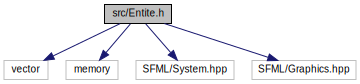
\includegraphics[width=350pt]{_entite_8h__incl}
\end{center}
\end{figure}
Ce graphe montre quels fichiers incluent directement ou indirectement ce fichier \+:\nopagebreak
\begin{figure}[H]
\begin{center}
\leavevmode
\includegraphics[width=350pt]{_entite_8h__dep__incl}
\end{center}
\end{figure}
\subsection*{Classes}
\begin{DoxyCompactItemize}
\item 
class \hyperlink{class_entite}{Entite}
\begin{DoxyCompactList}\small\item\em Classe virtuelle qui définit une entité \end{DoxyCompactList}\end{DoxyCompactItemize}

\hypertarget{_input_8cpp}{}\section{Référence du fichier src/\+Interface/\+Input.cpp}
\label{_input_8cpp}\index{src/\+Interface/\+Input.\+cpp@{src/\+Interface/\+Input.\+cpp}}
{\ttfamily \#include \char`\"{}Input.\+h\char`\"{}}\newline
{\ttfamily \#include $<$cmath$>$}\newline
Graphe des dépendances par inclusion de Input.\+cpp\+:\nopagebreak
\begin{figure}[H]
\begin{center}
\leavevmode
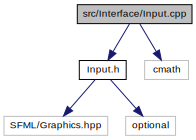
\includegraphics[width=269pt]{_input_8cpp__incl}
\end{center}
\end{figure}

\hypertarget{_input_8h}{}\section{Référence du fichier src/\+Interface/\+Input.h}
\label{_input_8h}\index{src/\+Interface/\+Input.\+h@{src/\+Interface/\+Input.\+h}}
{\ttfamily \#include $<$S\+F\+M\+L/\+Graphics.\+hpp$>$}\newline
{\ttfamily \#include $<$bitset$>$}\newline
{\ttfamily \#include \char`\"{}../constantes.\+h\char`\"{}}\newline
{\ttfamily \#include \char`\"{}../\+Utilitaires/optional.\+h\char`\"{}}\newline
Graphe des dépendances par inclusion de Input.\+h\+:
% FIG 0
Ce graphe montre quels fichiers incluent directement ou indirectement ce fichier \+:
% FIG 1
\subsection*{Classes}
\begin{DoxyCompactItemize}
\item 
class \hyperlink{class_input__base}{Input\+\_\+base$<$ N $>$}
\end{DoxyCompactItemize}
\subsection*{Définitions de type}
\begin{DoxyCompactItemize}
\item 
using \hyperlink{_input_8h_a5588d60d674991c719a8df848313e966}{Input} = \hyperlink{class_input__base}{Input\+\_\+base}$<$ \hyperlink{constantes_8h_a726db5d0e2803e025a8677641c60887b}{N\+B\+\_\+\+A\+C\+T\+I\+ON} $>$
\end{DoxyCompactItemize}


\subsection{Documentation des définitions de type}
\mbox{\Hypertarget{_input_8h_a5588d60d674991c719a8df848313e966}\label{_input_8h_a5588d60d674991c719a8df848313e966}} 
\index{Input.\+h@{Input.\+h}!Input@{Input}}
\index{Input@{Input}!Input.\+h@{Input.\+h}}
\subsubsection{\texorpdfstring{Input}{Input}}
{\footnotesize\ttfamily using \hyperlink{_input_8h_a5588d60d674991c719a8df848313e966}{Input} =  \hyperlink{class_input__base}{Input\+\_\+base}$<$\hyperlink{constantes_8h_a726db5d0e2803e025a8677641c60887b}{N\+B\+\_\+\+A\+C\+T\+I\+ON}$>$}


\hypertarget{main_8cpp}{}\section{Référence du fichier src/main.cpp}
\label{main_8cpp}\index{src/main.\+cpp@{src/main.\+cpp}}
{\ttfamily \#include $<$S\+F\+M\+L/\+Graphics.\+hpp$>$}\newline
{\ttfamily \#include $<$cmath$>$}\newline
{\ttfamily \#include $<$ctime$>$}\newline
{\ttfamily \#include $<$iostream$>$}\newline
{\ttfamily \#include \char`\"{}constantes.\+h\char`\"{}}\newline
{\ttfamily \#include \char`\"{}Entite.\+h\char`\"{}}\newline
{\ttfamily \#include \char`\"{}Utilitaires/\+Collision.\+h\char`\"{}}\newline
{\ttfamily \#include \char`\"{}Partie.\+h\char`\"{}}\newline
Graphe des dépendances par inclusion de main.\+cpp\+:\nopagebreak
\begin{figure}[H]
\begin{center}
\leavevmode
\includegraphics[width=350pt]{main_8cpp__incl}
\end{center}
\end{figure}
\subsection*{Fonctions}
\begin{DoxyCompactItemize}
\item 
int \hyperlink{main_8cpp_ae66f6b31b5ad750f1fe042a706a4e3d4}{main} ()
\end{DoxyCompactItemize}


\subsection{Documentation des fonctions}
\mbox{\Hypertarget{main_8cpp_ae66f6b31b5ad750f1fe042a706a4e3d4}\label{main_8cpp_ae66f6b31b5ad750f1fe042a706a4e3d4}} 
\index{main.\+cpp@{main.\+cpp}!main@{main}}
\index{main@{main}!main.\+cpp@{main.\+cpp}}
\subsubsection{\texorpdfstring{main()}{main()}}
{\footnotesize\ttfamily int main (\begin{DoxyParamCaption}{ }\end{DoxyParamCaption})}

le truc que Cyril avait tapé jeudi 7 en club

$<$attention très bordélique 
\hypertarget{_partie_8cpp}{}\section{Référence du fichier src/\+Partie.cpp}
\label{_partie_8cpp}\index{src/\+Partie.\+cpp@{src/\+Partie.\+cpp}}
{\ttfamily \#include \char`\"{}Partie.\+h\char`\"{}}\newline
{\ttfamily \#include \char`\"{}\+\_\+projectiles.\+h\char`\"{}}\newline
{\ttfamily \#include \char`\"{}\+\_\+\+Capacites.\+h\char`\"{}}\newline
{\ttfamily \#include \char`\"{}Proj\+Test.\+h\char`\"{}}\newline
{\ttfamily \#include \char`\"{}Vaisseau\+Test.\+h\char`\"{}}\newline
Graphe des dépendances par inclusion de Partie.\+cpp\+:\nopagebreak
\begin{figure}[H]
\begin{center}
\leavevmode
\includegraphics[width=350pt]{_partie_8cpp__incl}
\end{center}
\end{figure}

\hypertarget{_partie_8h}{}\section{Référence du fichier src/\+Partie.h}
\label{_partie_8h}\index{src/\+Partie.\+h@{src/\+Partie.\+h}}
{\ttfamily \#include $<$vector$>$}\newline
{\ttfamily \#include $<$string$>$}\newline
{\ttfamily \#include $<$algorithm$>$}\newline
{\ttfamily \#include \char`\"{}Capacite.\+h\char`\"{}}\newline
{\ttfamily \#include \char`\"{}Projectile.\+h\char`\"{}}\newline
{\ttfamily \#include \char`\"{}Vaisseau.\+h\char`\"{}}\newline
Graphe des dépendances par inclusion de Partie.\+h\+:\nopagebreak
\begin{figure}[H]
\begin{center}
\leavevmode
\includegraphics[width=323pt]{_partie_8h__incl}
\end{center}
\end{figure}
\subsection*{Classes}
\begin{DoxyCompactItemize}
\item 
class \hyperlink{class_partie}{Partie}
\begin{DoxyCompactList}\small\item\em Description brève. \end{DoxyCompactList}\end{DoxyCompactItemize}

\hypertarget{_projectile_8cpp}{}\section{src/\+Projectiles/\+Projectile.cpp File Reference}
\label{_projectile_8cpp}\index{src/\+Projectiles/\+Projectile.\+cpp@{src/\+Projectiles/\+Projectile.\+cpp}}
{\ttfamily \#include \char`\"{}Projectile.\+h\char`\"{}}\newline
{\ttfamily \#include $<$climits$>$}\newline

\hypertarget{_projectile_8h}{}\section{Référence du fichier src/\+Projectiles/\+Projectile.h}
\label{_projectile_8h}\index{src/\+Projectiles/\+Projectile.\+h@{src/\+Projectiles/\+Projectile.\+h}}
{\ttfamily \#include $<$vector$>$}\newline
{\ttfamily \#include $<$string$>$}\newline
{\ttfamily \#include $<$algorithm$>$}\newline
{\ttfamily \#include \char`\"{}../\+Entite.\+h\char`\"{}}\newline
Graphe des dépendances par inclusion de Projectile.\+h\+:
% FIG 0
Ce graphe montre quels fichiers incluent directement ou indirectement ce fichier \+:
% FIG 1
\subsection*{Classes}
\begin{DoxyCompactItemize}
\item 
class \hyperlink{class_projectile}{Projectile}
\begin{DoxyCompactList}\small\item\em Classe abstraite qui définit la structure générale d\textquotesingle{}un projectile, à faire hériter pour chaque projectile. \end{DoxyCompactList}\end{DoxyCompactItemize}

\hypertarget{_projectile_piou_piou_8cpp}{}\section{Référence du fichier src/\+Projectiles/\+Projectile\+Piou\+Piou.cpp}
\label{_projectile_piou_piou_8cpp}\index{src/\+Projectiles/\+Projectile\+Piou\+Piou.\+cpp@{src/\+Projectiles/\+Projectile\+Piou\+Piou.\+cpp}}

\hypertarget{_projectile_piou_piou_8h}{}\section{Référence du fichier src/\+Projectiles/\+Projectile\+Piou\+Piou.h}
\label{_projectile_piou_piou_8h}\index{src/\+Projectiles/\+Projectile\+Piou\+Piou.\+h@{src/\+Projectiles/\+Projectile\+Piou\+Piou.\+h}}
\subsection*{Classes}
\begin{DoxyCompactItemize}
\item 
class \hyperlink{class_projectile_piou_piou}{Projectile\+Piou\+Piou}
\end{DoxyCompactItemize}

\hypertarget{_proj_piou_8cpp}{}\section{Référence du fichier src/\+Projectiles/\+Proj\+Piou.cpp}
\label{_proj_piou_8cpp}\index{src/\+Projectiles/\+Proj\+Piou.\+cpp@{src/\+Projectiles/\+Proj\+Piou.\+cpp}}
{\ttfamily \#include \char`\"{}Proj\+Piou.\+h\char`\"{}}\newline
{\ttfamily \#include $<$cmath$>$}\newline
Graphe des dépendances par inclusion de Proj\+Piou.\+cpp\+:
% FIG 0

\hypertarget{_proj_piou_8h}{}\section{Référence du fichier src/\+Projectiles/\+Proj\+Piou.h}
\label{_proj_piou_8h}\index{src/\+Projectiles/\+Proj\+Piou.\+h@{src/\+Projectiles/\+Proj\+Piou.\+h}}
{\ttfamily \#include \char`\"{}Projectile.\+h\char`\"{}}\newline
Graphe des dépendances par inclusion de Proj\+Piou.\+h\+:
\nopagebreak
\begin{figure}[H]
\begin{center}
\leavevmode
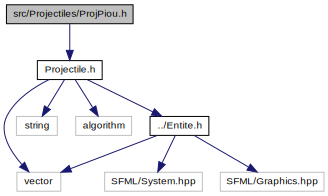
\includegraphics[width=350pt]{_proj_piou_8h__incl}
\end{center}
\end{figure}
Ce graphe montre quels fichiers incluent directement ou indirectement ce fichier \+:
\nopagebreak
\begin{figure}[H]
\begin{center}
\leavevmode
\includegraphics[width=350pt]{_proj_piou_8h__dep__incl}
\end{center}
\end{figure}
\subsection*{Classes}
\begin{DoxyCompactItemize}
\item 
class \hyperlink{class_proj_piou}{Proj\+Piou}
\end{DoxyCompactItemize}

\hypertarget{_proj_test_8cpp}{}\section{Référence du fichier src/\+Projectiles/\+Proj\+Test.cpp}
\label{_proj_test_8cpp}\index{src/\+Projectiles/\+Proj\+Test.\+cpp@{src/\+Projectiles/\+Proj\+Test.\+cpp}}
{\ttfamily \#include \char`\"{}Proj\+Test.\+h\char`\"{}}\newline
{\ttfamily \#include \char`\"{}../constantes.\+h\char`\"{}}\newline
Graphe des dépendances par inclusion de Proj\+Test.\+cpp\+:
\nopagebreak
\begin{figure}[H]
\begin{center}
\leavevmode
\includegraphics[width=350pt]{_proj_test_8cpp__incl}
\end{center}
\end{figure}

\hypertarget{_proj_test_8h}{}\section{Référence du fichier src/\+Proj\+Test.h}
\label{_proj_test_8h}\index{src/\+Proj\+Test.\+h@{src/\+Proj\+Test.\+h}}
{\ttfamily \#include \char`\"{}Projectile.\+h\char`\"{}}\newline
Graphe des dépendances par inclusion de Proj\+Test.\+h\+:\nopagebreak
\begin{figure}[H]
\begin{center}
\leavevmode
\includegraphics[width=350pt]{_proj_test_8h__incl}
\end{center}
\end{figure}
Ce graphe montre quels fichiers incluent directement ou indirectement ce fichier \+:\nopagebreak
\begin{figure}[H]
\begin{center}
\leavevmode
\includegraphics[width=350pt]{_proj_test_8h__dep__incl}
\end{center}
\end{figure}
\subsection*{Classes}
\begin{DoxyCompactItemize}
\item 
class \hyperlink{class_proj_test}{Proj\+Test}
\end{DoxyCompactItemize}

\hypertarget{_vaisseau_8cpp}{}\section{Référence du fichier src/\+Vaisseau.cpp}
\label{_vaisseau_8cpp}\index{src/\+Vaisseau.\+cpp@{src/\+Vaisseau.\+cpp}}
{\ttfamily \#include $<$vector$>$}\newline
{\ttfamily \#include $<$string$>$}\newline
{\ttfamily \#include $<$algorithm$>$}\newline
{\ttfamily \#include \char`\"{}Capacite.\+h\char`\"{}}\newline
{\ttfamily \#include \char`\"{}Vaisseau.\+h\char`\"{}}\newline
{\ttfamily \#include \char`\"{}Projectile.\+h\char`\"{}}\newline
Graphe des dépendances par inclusion de Vaisseau.\+cpp\+:\nopagebreak
\begin{figure}[H]
\begin{center}
\leavevmode
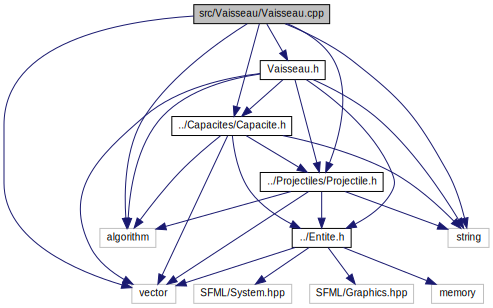
\includegraphics[width=328pt]{_vaisseau_8cpp__incl}
\end{center}
\end{figure}

\hypertarget{_vaisseau_8h}{}\section{Référence du fichier src/\+Vaisseau/\+Vaisseau.h}
\label{_vaisseau_8h}\index{src/\+Vaisseau/\+Vaisseau.\+h@{src/\+Vaisseau/\+Vaisseau.\+h}}
{\ttfamily \#include $<$vector$>$}\newline
{\ttfamily \#include $<$string$>$}\newline
{\ttfamily \#include $<$algorithm$>$}\newline
{\ttfamily \#include \char`\"{}../\+Capacites/\+Capacite.\+h\char`\"{}}\newline
{\ttfamily \#include \char`\"{}../\+Entite.\+h\char`\"{}}\newline
{\ttfamily \#include \char`\"{}../\+Projectiles/\+Projectile.\+h\char`\"{}}\newline
{\ttfamily \#include \char`\"{}../\+Interface/\+Input.\+h\char`\"{}}\newline
Graphe des dépendances par inclusion de Vaisseau.\+h\+:\nopagebreak
\begin{figure}[H]
\begin{center}
\leavevmode
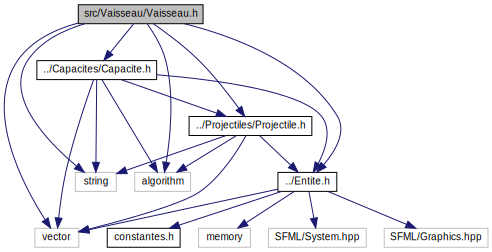
\includegraphics[width=350pt]{_vaisseau_8h__incl}
\end{center}
\end{figure}
Ce graphe montre quels fichiers incluent directement ou indirectement ce fichier \+:\nopagebreak
\begin{figure}[H]
\begin{center}
\leavevmode
\includegraphics[width=350pt]{_vaisseau_8h__dep__incl}
\end{center}
\end{figure}
\subsection*{Classes}
\begin{DoxyCompactItemize}
\item 
class \hyperlink{class_vaisseau}{Vaisseau}
\begin{DoxyCompactList}\small\item\em classe du vaisseau (véhicule) d\textquotesingle{}un joueur ou d\textquotesingle{}un ennemi \end{DoxyCompactList}\end{DoxyCompactItemize}

\hypertarget{_vaisseau_test_8cpp}{}\section{src/\+Vaisseau/\+Vaisseau\+Test.cpp File Reference}
\label{_vaisseau_test_8cpp}\index{src/\+Vaisseau/\+Vaisseau\+Test.\+cpp@{src/\+Vaisseau/\+Vaisseau\+Test.\+cpp}}
{\ttfamily \#include \char`\"{}Vaisseau\+Test.\+h\char`\"{}}\newline
{\ttfamily \#include $<$cmath$>$}\newline

\hypertarget{_vaisseau_test_8h}{}\section{Référence du fichier src/\+Vaisseau/\+Vaisseau\+Test.h}
\label{_vaisseau_test_8h}\index{src/\+Vaisseau/\+Vaisseau\+Test.\+h@{src/\+Vaisseau/\+Vaisseau\+Test.\+h}}
{\ttfamily \#include \char`\"{}Vaisseau.\+h\char`\"{}}\newline
{\ttfamily \#include \char`\"{}../\+Capacites/\+Capacite.\+h\char`\"{}}\newline
Graphe des dépendances par inclusion de Vaisseau\+Test.\+h\+:
\nopagebreak
\begin{figure}[H]
\begin{center}
\leavevmode
\includegraphics[width=350pt]{_vaisseau_test_8h__incl}
\end{center}
\end{figure}
Ce graphe montre quels fichiers incluent directement ou indirectement ce fichier \+:
\nopagebreak
\begin{figure}[H]
\begin{center}
\leavevmode
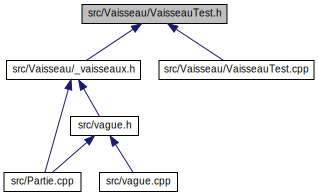
\includegraphics[width=330pt]{_vaisseau_test_8h__dep__incl}
\end{center}
\end{figure}
\subsection*{Classes}
\begin{DoxyCompactItemize}
\item 
class \hyperlink{class_vaisseau_test}{Vaisseau\+Test}
\end{DoxyCompactItemize}

%--- End generated contents ---

% Index
\backmatter
\newpage
\phantomsection
\clearemptydoublepage
\addcontentsline{toc}{chapter}{Index}
\printindex

\end{document}
